

\paragraph{\textswab{Spin chain types}}

Some of the most common examples of spin chains are treated as follows, 

\begin{itemize}
    \item The simplest example of a $SU(2)$-symmetric spin Hamiltonian is therefore the XXX-nearest-neighbour Heisenberg model, where 

\begin{equation}
    \Hamiltonian_{\mathds{X}\mathds{X}\mathds{X}} = -J \sum_{\langle ij \rangle} {\spin}_i \cdot {\spin}_j = -J \sum_{i=1}^{N} \bigg(\frac{1}{2} (\sigma_i^+ \sigma_{i+1}^{-} + \sigma_i^- \sigma_{i+1}^+) + \frac{1}{4} \sigma_i^z \sigma_{i+1}^z\bigg),
\end{equation}

where in the ferromagnetic case the diagonal terms in the Hamiltonian favour aligned spins, while in the antiferromagnetic case, the diagonal terms favour antialignement. The XXX-Hamiltonian commutes with the magnetization operator by construction. Note that Schur's lemma does not immediately apply since the magnetization operator is reducible. \\

\item The XXZ model is a deformation of the Heisenberg model, breaking the $SU(2)$-model symmetry down to a $U(1)$-subgroup. The XXZ-hamiltonian reads

\begin{equation}
    \Hamiltonian_{\mathds{X}\mathds{X}\mathds{Z}} = - \sum_{\langle jk \rangle} (J_\perp (\spin_j^x \spin_k^x + \spin_j^y \spin_k^y) + J_z \spin_j^z \spin_k^z) = - \sum_{j=1}^{N} \bigg( J_\perp (\sigma_{j}^+ \sigma_{j+1}^- + \sigma_{j}^- \sigma_{j+1}^+) + \frac{\Delta}{2} \sigma_j^z \sigma_{j+1}^z \bigg),
    \label{XXZ hamiltonian}
\end{equation}

which is the most general $U(1)$-symmetric nearest-neighbor interaction for spin-$\frac{1}{2}$ particles. \\

Although this model is no longer $SU(2)$-symmetric, the magnetization operator commutes with the hamiltonian, thus generating a $U(1)$-symmetry. Even though the full $SU(2)$-symmetry is broken, the degrees of freedom are still typically referred to as spins. The sign of $J_z$ alone determines whether the model is ferromagnetic, $J_z > 0$, or antiferromagnetic, $J_z < 0$, since the sign of $J_\perp$ is unimportant in any bipartite lattice, redefining the states by changing the overall sign of the $\spin^x$ and $\spin^y$-operators on half the lattice sites, leaves the algebra unchanged but flips the sign of $J_\perp$. Therefore, the physically meaningful coupling is $\Delta = \frac{J_z}{|J_\perp|}$, so that $\Delta = \pm 1$ for the ferromagnetic and antiferromagnetic spin models, respectively. In the $\Delta \rightarrow \pm \infty$-limit, only the $J_z$ remains, and the model is effectively classical. For the ferromagnetic case $J_z > 0$, all the spins simply line up with the maximum value of ${\bf M}^z$. In the antiferromagnetic case, $\Delta \rightarrow -\infty$ on a bipartite lattice, the spins take their maximum opposite values on every other site. \\

It is easy to check that this Hamiltonian commutes with the magnetization operator, and so preserves a $U(1)\times \mathds{Z}_2$-symmetry. In a classical notion, the $U(1)$-symmetry corresponds to rotations around the $z$-axis, while the $\mathds{Z}_2$ corresponds to flipping all the spins ${\spin_j^a \rightarrow -\spin_j^a}$. \\

\item A still more general Hamiltonian is given by the XYZ-model, which only preserves the spin-flip symmetry. 
\end{itemize}

None of these Hamiltonians correspond to a quantum version of the Ising model. \\

\subsubsection{\textit{Quantum Ising Model}}

\clearpage

\subsubsection{\textit{Bethe ansatz for the XXX-model}}

\paragraph{\textswab{Heisenberg XXX-chain}}

Consider a one-dimensional lattice with $N$ lattice sites and a $\frac{1}{2}$-spin particle positioned at every lattice site, which have a nearest neighbour spin-spin interaction. Each particles either has spin up or spin down, generating a two-dimensional local Hilbert space, $\vds_n$. Strictly speaking there are two possible topologies for a one-dimensional chain, open or closed. Consider the XXX-Hamiltonian with closed topology, given by 

\begin{equation}
\begin{split}
    {\bf H} &= J \sum_{n=1}^{N} \bigg(\vec{\spin}_n \cdot \vec{\spin}_{n+1} - \frac{1}{4} \mathds{1}^{\otimes N} \bigg) = \frac{J}{4}\sum_{n=1}^{N} \bigg(\vec{\sigma}_n \cdot \vec{\sigma}_{n+1} - \frac{1}{4} \mathds{1}^{\otimes N} \bigg).
    \label{XXX model}
\end{split}
\end{equation}

Note that $J < 0$ models a ferromagnetic state while $J > 0$ models an anti-ferromagnetic state. A ferromagnetic state refers to a state where all the spins are alligned while an anti-ferromagnetic state refers to a state where adjacent spins are anti-aligned within the domain. \\

\begin{tcolorbox}[colback =yellow,title = Physical Context]

The main point of the Bethe solution is that XXX Heisenberg Hamiltonian, which defines the model, can be expressed in terms of a complex-valued $\bm{\mathcal R}$-matrix which is a solution of the Yang-Baxter equation, thus leading to the model's integrability. The most convenient approach is to construct a transfer $\bm{\mathcal{T}}$-matrix -a one parameter commutative family of operators acting on the full state space of the Heisenberg spin chain. 

\end{tcolorbox}

\blanky \\ 

\paragraph{\textswab{Some fundamentals of Matrix Theory}}

Let $\mathds{V}$ be an $n$-dimensional $\mathds{C}$-vector space and let $k \in \mathds{1}_n \textnormal{ such that } \in \mathds{N}_{[0, k]}$. Let $\mathfrak{J} = \mathds{1}_n / \mathds{1}_k = \{k+1,\cdots, n\}$. Let $A \in \textnormal{GL}(n, \mathds{C})$, which can be written in block notation as 
\begin{equation}
    A = \left(\begin{array}{cc}
        A_{\mathcal{I}} & A_{\mathcal{I} \mathfrak{J}}  \\
        A_{\mathfrak{J} \mathcal{I}} & A_{\mathfrak{J}}
    \end{array}\right) \begin{array}{c}
         \mathds{C}^k  \\
         \mathds{C}^{n-k}
    \end{array} \textnormal{ where } \begin{array}{cc}
        A_{\mathcal{I}} \in \textnormal{GL}(k, \mathds{C}),  &  A_{\mathcal{I} \mathfrak{J}} \in \textnormal{GL}(k \rightarrow n-k, \mathds{C}), \\
        A_{\mathfrak{J} \mathcal{I}} \in  \textnormal{GL}(n-k \rightarrow k, \mathds{C}), & A_{\mathfrak{J}}  \in \textnormal{GL}(n-k, \mathds{C}),
    \end{array} 
\end{equation}

This notation is consistent with the common matrix operations. The same idea holds for writing down a  block matrix representation for a linear operator with respect to a given subspace. Let $\mathcal{S} \subset \mathds{C}^n$ be a $k$-dimensional vector subspace, such that $\mathds{C}^n = \mathcal{S} \oplus \mathcal{S}^{\perp}$. Then, every linear operator in $\textnormal{End}(\mathds{C}^n)$ can be rewritten as a $\twobytwo$-block-matrix, with its entries being matrices of a given dimension ie. \footnote{
For example, consider the orthogonal projector over $\mathcal{S}$, labelled $P_{\mathcal{S}}$. In this notation, its matrix representation is given by 

\begin{equation*}
    P_{\mathcal{S}} = \left( \begin{array}{cc}
       \mathcal{I} & 0 \\
       0 & 0
    \end{array} \right) \begin{array}{c}
         \mathcal{S} \\
         \mathcal{S}^\perp
    \end{array} 
\end{equation*}}

\begin{equation*}
\begin{split}
    A \in \textnormal{End}(\mathds{C}^n) &\rightarrow \exists! \left\{\begin{array}{cc}
        A_{\mathcal{S}} \in \textnormal{GL}(k, \mathds{C}),  &  A_{\mathcal{S}, \mathcal{S}^\perp} \in \textnormal{GL}(k \rightarrow n-k, \mathds{C}), \\
        A_{\mathcal{S}^\perp, \mathcal{S}}  \in \textnormal{GL}(n-k \rightarrow k, \mathds{C}), & A_{\mathcal{S}^\perp} \in \textnormal{GL}(n-k, \mathds{C}),
    \end{array} \right\} / \\
   &A = \left( \begin{array}{cc}
       A_{\mathcal{S}} & A_{\mathcal{S}, \mathcal{S}^\perp}  \\
       A_{\mathcal{S}^\perp, \mathcal{S}} & A_{\mathcal{S}^\perp} 
    \end{array} \right) \begin{array}{c}
         \mathcal{S} \\
         \mathcal{S}^\perp
    \end{array}
    \end{split}
\end{equation*}

The main idea behind the lax-operator and $\bm{\mathcal{R}}$-operator methods is to find an operator, eg. a product-matrix, where each one of the matrices acts non-trivially only on a single Hilbert space $\vds \simeq \ctwo$. Said matrices can then be rewritten in the previous form. \\

\paragraph{\textswab{The Lax operator}} Consider an XXX-spin chain with $N$ sites and a corresponding Hilbert space given by 

\begin{align}
    \mathds{H} \simeq \bigotimes_{n=1}^{N} {\mathds{V}_n} \textnormal{ where } {\mathds{V}_n} \simeq \ctwo \begin{array}{c}
         \textnormal{To these individual Hilbert spaces, additional}  \\
         \textnormal{auxiliary, non-physical, spaces $\mathds{V}_a \simeq \ctwo$, can be added. } \\
    \end{array}
\end{align}

The algebraic Bethe ansatz' basic tool is the lax operator $\bm{\mathcal{L}}$, whose definition is as follows. 

\begin{df}
   The lax operator $\bm{\mathcal{L}}$ can be defined as an operator which involves the local quantum space $\mathds{V}_n$ and the auxiliary space $\mathds{V}_a$, as follows 

\begin{equation}
    \begin{array}{c}
         \bm{\mathcal{L}} : \mathds{V}_n \otimes \mathds{V}_a \rightarrow \mathds{V}_n \otimes \mathds{V}_a \\
         \bm{\mathcal{L}}_{n, a} = u(\mathds{1}_n \otimes \mathds{1}_a) + i \sum_{\alpha} \spin_n^\alpha \otimes \sigma_{a}^\alpha, \blanky \forall n \leq N \\
         %= u^{\mu} {S}_{\nu} \sigma^{\nu} \textnormal{ where $u^{\mu} = (u, i,i,i)$}
    \end{array} \begin{array}{c}
         \textnormal{ where $\mathds{1}_n$ and $\spin_n^\alpha$ act on $\mathds{V}_n $} \\
         \textnormal{ while $\mathds{1}_a$ and $\spin_a^\alpha$ act upon $\mathds{V}_a$ and where the}       \\
         \textnormal{ complex-valued $u$-parameter is the spectral parameter.}
    \end{array}
    \label{lax operator}
\end{equation}
\end{df}

 Note that \cref{lax operator} can be rewritten as 

\begin{equation}
    \begin{split}
    \bm{\mathcal{L}}_{n, a} &= u(\mathds{1}_n \otimes \mathds{1}_a) + i \sum_{\alpha} \spin_n^\alpha \otimes \sigma_{a}^\alpha 
    %&= u \left(\begin{array}{cc}
    %    \mathds{1}_n & 0  \\
    %    0 & \mathds{1}_a 
    %\end{array}\right) + i \spin^{x}_{n} \otimes \left(\begin{array}{cc}
    %    0 & 1 \\
    %    1 & 0
    %\end{array}\right)_a + i \spin^{y}_{n} \otimes \left(\begin{array}{cc}
    %    0 & -i \\
    %    i & 0 
    %\end{array}\right)_a + i \spin^{z}_{n} \otimes \left(\begin{array}{cc}
    %    1 & 0  \\
    %    0 & -1
    %\end{array}\right)_a \\
    = \left(\begin{array}{cc}
       u \mathds{1}_n + i \spin^{z}_{n} & i \spin^{x}_{n} + \spin^{y}_{n} \\
       i \spin^{x}_{n} - \spin^{y}_{n}  & u \mathds{1}_n - i \spin^{z}_{n}
    \end{array}\right)_a = \left(\begin{array}{cc}
       u \mathds{1}_n + i \spin^{z}_{n} & i \spin^{-}_{n} \\
       i \spin^{+}_{n} & u \mathds{1}_n - i \spin^{z}_{n}
    \end{array}\right)_a,
    \end{split}
\end{equation}
    
which is a $2 \times 2$-matrix in the auxiliary space $\mathds{V}_a$ and the matrix entries are operators acting on the physical Hilbert space $\mathds{V}_n$. Consider now the following mathematical object. 

\begin{df}
    Let the permutation operator be
    
    \begin{equation}
        \bm{\mathcal P}_{n,a} = \frac{1}{2} \bigg(\mathds{1}_n \otimes \mathds{1}_a + \sum_{\alpha}\sigma_n^{\alpha}  \otimes \sigma_n^{\alpha} \bigg) = \frac{1}{2} \sigma^{n \mu}\sigma^{\alpha}_{\mu}
        \label{permutation op}
    \end{equation}
    
    which \footnote{Note that the permutation operator can be written as a $2 \times 2$-matrix in the auxiliary space $\mathds{V}_a$,
\begin{equation} 
\begin{split}
    \bm{\mathcal P}_{n,a} &= \frac{1}{2} \left[ \left(\begin{array}{cc}
        \mathds{1}_n & 0  \\
        0 & \mathds{1}_a 
    \end{array}\right) + \sigma^{x}_{n} \otimes \left(\begin{array}{cc}
        0 & 1 \\
        1 & 0
    \end{array}\right)_a + \sigma^{y}_{n} \otimes \left(\begin{array}{cc}
        0 & -i \\
        i & 0 
    \end{array}\right)_a + \sigma^{z}_{n} \otimes \left(\begin{array}{cc}
        1 & 0  \\
        0 & -1
    \end{array}\right)_a \right] \\
    &= \left(\begin{array}{cc}
       \mathds{1}_n + \sigma^{z}_{n} &  \sigma^{x}_{n} - i\sigma^{y}_{n} \\
       \sigma^{x}_{n} + i\sigma^{y}_{n}  & \mathds{1}_n - \sigma^{z}_{n}
    \end{array}\right)_a = 
    %\left(\begin{array}{cccc}
    %    1 & 0 & 0 & 0   \\
    %    0 & 0 & 1 & 0   \\
    %    0 & 1 & 0 & 0   \\
    %    0 & 0 & 0 & 1
    %\end{array}\right)
    \end{split}
\end{equation}} acts on both the physical and auxiliary systems.
\end{df}

Using this definition for the permutation operator, the lax operator can then be rewritten as

\begin{equation}
    \begin{split}
       \bm{\mathcal{L}}_{n, a} &= u(\mathds{1}_n \otimes \mathds{1}_a) + i \sum_{\alpha} \spin_n^\alpha \otimes \sigma_{a}^\alpha = u(\mathds{1}_n \otimes \mathds{1}_a) + \frac{i}{2} \sum_{\alpha} \sigma_n^\alpha \otimes \sigma_{a}^\alpha \\
       &= u(\mathds{1}_n \otimes \mathds{1}_a) - \frac{i}{2} (\mathds{1}_n \otimes \mathds{1}_a) + \frac{i}{2} (\mathds{1}_n \otimes \mathds{1}_a) + \frac{i}{2} \sum_{\alpha} \sigma_n^\alpha \otimes \sigma_{a}^\alpha \\
       &= \bigg(u-\frac{i}{2}\bigg) (\mathds{1}_n \otimes \mathds{1}_a) + \frac{i}{2} \bigg( \mathds{1}_n \otimes \mathds{1}_a + \sum_{\alpha}\sigma_n^{\alpha}  \otimes \sigma_n^{\alpha} \bigg) \\
       &= \bigg(u-\frac{i}{2}\bigg) \mathds{1}_{n, a} + i \bm{\mathcal{P}}_{n, a}.
       \end{split}
       \label{l-matrix def}
\end{equation}

\blanky \\

\paragraph{\textswab{Fundamental commutation Relations and Monodromy Matrix}}

Consider the following two lax operators

\begin{equation*}
    \begin{array}{c}
        \bl_{n, a_1}(u_1): \blanky \vds_n \otimes \vds_{a_1} \rightarrow \vds_n \otimes \vds_{a_1}  \\
        \\
        \bl_{n, a_2}(u_2): \blanky \vds_n \otimes \vds_{a_2} \rightarrow \vds_n \otimes \vds_{a_2} 
    \end{array} \begin{array}{c}
         \textnormal{both of which act on the physical quantum}\\
         \textnormal{state and on two different auxiliary spaces as well}\footnote{
The permutation operator indeed permutes the factors in the tensor product the factors in the tensor product by calculating the sum of tensor product of the Pauli matrices with respect to the standard four-dimensional basis, ie. if $\x = \left(\begin{array}{c}
     a \\
     b 
\end{array}\right)$ and ${\bf y} = \left(\begin{array}{c}
     c \\
     d 
\end{array}\right)$ then $\x \otimes {\bf y} = \left( \begin{array}{cc}
    ac & ad  \\
    bc & bd 
\end{array} \right)$ and  ${\bf y} \otimes \x = \left( \begin{array}{cc}
    ac & bc  \\
    ad & bd 
\end{array} \right)$. Therefore,

\begin{equation}
    \bm{\mathcal{P}}_{n, a} (\x \otimes {\bf y} ) = {\bf y} \otimes \x \textnormal{ and } \bm{\mathcal{P}}_{n, a} ( {\bf y} \otimes \x) = \x \otimes {\bf y}.
\end{equation}} 
    \end{array}
\end{equation*}

The product of these two operator is then a triple tensor product in $\mathds{V}_{n} \otimes \mathds{V}_{a_1} \otimes \mathds{V}_{a_2}$. Now, the following matrix arises 

\begin{df}
Consider an $\bm{\mathcal{R}}$-matrix which relates the permutation and spectral parameters of two auxiliary spaces, which is given by  

\begin{equation}
\begin{array}{c}
     \bm{\mathcal{R}}: \blanky \mathds{V}_{a_1} \otimes \mathds{V}_{a_2} \otimes \mathds{V}_{a_1} \otimes \mathds{V}_{a_2} \\ 
     \\
     \bm{\mathcal{R}}_{a_1, a_2}(u_1-u_2) = (u_1-u_2) \mathds{1}_{a_1, a_2} + i \bm{\mathcal{P}}_{a_1, a_2}, \\
     \label{R-matrix def}
\end{array}
\end{equation}

which doesn't act on the physical system at all, but on the auxiliary, phantom, systems\footnote{Note that $\bm{\mathcal{R}}$ can be rewritten as a $\twobytwo$-matrix in either of the auxiliary spaces, as follows

\begin{equation}
    \bm{\mathcal{R}}_{a1, a2} = \left(\begin{array}{cc}
        \bigg(u + \frac{i}{2}\bigg) \mathds{1}_{a_2} + i \spin_{a_2}^z & i \spin_{a_2}^{-} \\
        i \spin_{a_2}^{+}  & \bigg(u + \frac{i}{2}\bigg) \mathds{1}_{a_2} - i \spin_{a_2}^z 
    \end{array} \right)_{a_1} = \left(\begin{array}{cc}
        \bigg(u + \frac{i}{2}\bigg) \mathds{1}_{a_1} + i \spin_{a_1}^z & i \spin_{a_1}^{-} \\
        i \spin_{a_1}^{+}  & \bigg(u + \frac{i}{2}\bigg) \mathds{1}_{a_1} - i \spin_{a_2}^z 
    \end{array} \right)_{a_2}.
\end{equation}}.
\end{df}

An interesting relationship between the products of the two lax operators and the $\bm{\mathcal{R}}$-matrix can then be found\footnote{Note that the following permutation properties hold 

\begin{equation}
\bm{\mathcal{P}}_{n, a_1}\bm{\mathcal{P}}_{n, a_2} = \bm{\mathcal{P}}_{a_1, a_2}\bm{\mathcal{P}}_{n, a_1} = \bm{\mathcal{P}}_{n, a_2}\bm{\mathcal{P}}_{a_2, a_1} \textnormal{ and } \bm{\mathcal{P}}_{a, b} = \bm{\mathcal{P}}_{b, a}
\end{equation}

}, consider 

\begin{align*}
    \bm{\mathcal{R}}_{a_1, a_2}(u_1-u_2) & \bm{\mathcal{L}}_{n, a_1} (u_1) \bm{\mathcal{L}}_{n, a_2} (u_2) \\ 
    &= {\bigg((u_1-u_2) \mathds{1}_{a_1, a_2} 
    + i \bm{\mathcal{P}}_{a_1, a_2}\bigg)}   \left(\bigg(u-\frac{i}{2}\bigg) \mathds{1}_{n, a_1} + i \bm{\mathcal{P}}_{n, a_1}\right) \left(\bigg(u-\frac{i}{2}\bigg) \mathds{1}_{n, a_2} + i \bm{\mathcal{P}}_{n, a_2}\right) \\
    &= \left({(u_1-u_2) \mathds{1}_{a_1, a_2} \bigg(u-\frac{i}{2}\bigg) \mathds{1}_{n, a_1}} + {(u_1-u_2) \mathds{1}_{a_1, a_2} i \bm{\mathcal{P}}_{n, a_1}} + i \bm{\mathcal{P}}_{a_1, a_2} \bigg(u-\frac{i}{2}\bigg) \mathds{1}_{n, a_1} + i^2 \bm{\mathcal{P}}_{a_1, a_2}  \bm{\mathcal{P}}_{n, a_1} \right) \\
    & \times \left(\bigg(u-\frac{i}{2}\bigg) \mathds{1}_{n, a_2} + i \bm{\mathcal{P}}_{n, a_2}\right) \\
    &= {(u_1-u_2) \mathds{1}_{a_1, a_2} \bigg(u-\frac{i}{2}\bigg) \mathds{1}_{n, a_1}} \bigg(u-\frac{i}{2}\bigg) \mathds{1}_{n, a_2} + {(u_1-u_2) \mathds{1}_{a_1, a_2} \bigg(u-\frac{i}{2}\bigg) \mathds{1}_{n, a_1}} i \bm{\mathcal{P}}_{n, a_2} \\
    &+ {(u_1-u_2) \mathds{1}_{a_1, a_2} i \bm{\mathcal{P}}_{n, a_1}} \bigg(u-\frac{i}{2}\bigg) \mathds{1}_{n, a_2} + {(u_1-u_2) \mathds{1}_{a_1, a_2} i \bm{\mathcal{P}}_{n, a_1}} i \bm{\mathcal{P}}_{n, a_2} \\ 
    &+ i \bm{\mathcal{P}}_{a_1, a_2} \bigg(u-\frac{i}{2}\bigg)\mathds{1}_{n, a_1}  \bigg(u-\frac{i}{2}\bigg) \mathds{1}_{n, a_2} + i \bm{\mathcal{P}}_{a_1, a_2} \bigg(u-\frac{i}{2}\bigg) \mathds{1}_{n, a_1} i \bm{\mathcal{P}}_{n, a_2} \\
    & - \bm{\mathcal{P}}_{a_1, a_2}  \bm{\mathcal{P}}_{n, a_1}  \bigg(u-\frac{i}{2}\bigg) \mathds{1}_{n, a_2} - \bm{\mathcal{P}}_{a_1, a_2}  \bm{\mathcal{P}}_{n, a_1} i \bm{\mathcal{P}}_{n, a_2} \\
    & = {(u_1-u_2) \mathds{1}_{a_1, a_2}  \bigg(u-\frac{i}{2}\bigg) \mathds{1}_{n, a_2}} \times \bigg(u-\frac{i}{2}\bigg) \mathds{1}_{n, a_1} + {(u_1-u_2) \mathds{1}_{a_1, a_2} i \bm{\mathcal{P}}_{n, a_2}} \times \bigg(u-\frac{i}{2}\bigg) \mathds{1}_{n, a_1} \\
    &+ {(u_1-u_2) \mathds{1}_{a_1, a_2} \bigg(u-\frac{i}{2}\bigg) \mathds{1}_{n, a_2}} \times  i \bm{\mathcal{P}}_{n, a_1} + {(u_1-u_2) \mathds{1}_{a_1, a_2} i \bm{\mathcal{P}}_{n, a_2}} \times i \bm{\mathcal{P}}_{n, a_1} \\
    &+ i \bm{\mathcal{P}}_{a_1, a_2} \bigg(u-\frac{i}{2}\bigg) \mathds{1}_{n, a_1}  \bigg(u-\frac{i}{2}\bigg) \mathds{1}_{n, a_2} + i \bm{\mathcal{P}}_{a_1, a_2} \bigg(u-\frac{i}{2}\bigg) \mathds{1}_{n, a_1} i \bm{\mathcal{P}}_{n, a_2} \\
    & - \bm{\mathcal{P}}_{a_1, a_2}  \bm{\mathcal{P}}_{n, a_1}  \bigg(u-\frac{i}{2}\bigg) \mathds{1}_{n, a_2} - \bm{\mathcal{P}}_{a_1, a_2}  \bm{\mathcal{P}}_{n, a_1} i \bm{\mathcal{P}}_{n, a_2}\end{align*}
\begin{align*} \\
    &= \left({(u_1-u_2) \mathds{1}_{a_1, a_2}  \bigg(u-\frac{i}{2}\bigg) \mathds{1}_{n, a_2}} + {(u_1-u_2) \mathds{1}_{a_1, a_2} i \bm{\mathcal{P}}_{n, a_2}}\right) \bigg(u-\frac{i}{2}\bigg) \mathds{1}_{n, a_1} \\
    &+ \left({(u_1-u_2) \mathds{1}_{a_1, a_2} \bigg(u-\frac{i}{2}\bigg) \mathds{1}_{n, a_2}} + {(u_1-u_2) \mathds{1}_{a_1, a_2} i \bm{\mathcal{P}}_{n, a_2}} \right) \times  i \bm{\mathcal{P}}_{n, a_1} \\
    &+ i \bm{\mathcal{P}}_{a_1, a_2} \bigg(u-\frac{i}{2}\bigg) \mathds{1}_{n, a_1} \bigg(u-\frac{i}{2}\bigg) \mathds{1}_{n, a_2} + i \bm{\mathcal{P}}_{a_1, a_2} \bigg(u-\frac{i}{2}\bigg) \mathds{1}_{n, a_1} i \bm{\mathcal{P}}_{n, a_2} \\
    & - \bm{\mathcal{P}}_{a_1, a_2}  \bm{\mathcal{P}}_{n, a_1}  \bigg(u-\frac{i}{2}\bigg) \mathds{1}_{n, a_2} - \bm{\mathcal{P}}_{a_1, a_2}  \bm{\mathcal{P}}_{n, a_1} i \bm{\mathcal{P}}_{n, a_2} \\
    &= \bigg((u_1-u_2) \mathds{1}_{a_1, a_2} \bigg(u-\frac{i}{2}\bigg) \mathds{1}_{n, a_2} + {(u_1-u_2) \mathds{1}_{a_1, a_2} i \bm{\mathcal{P}}_{n, a_2}} \bigg) \left( \bigg(u-\frac{i}{2}\bigg) \mathds{1}_{n, a_2} + i \bm{\mathcal{P}}_{n, a_1} \right) \\
    &+ i \bm{\mathcal{P}}_{a_1, a_2} \bigg(u-\frac{i}{2}\bigg) \mathds{1}_{n, a_1} \bigg(u-\frac{i}{2}\bigg) \mathds{1}_{n, a_2} + i \bm{\mathcal{P}}_{a_1, a_2} \bigg(u-\frac{i}{2}\bigg) \mathds{1}_{n, a_1} i \bm{\mathcal{P}}_{n, a_2} \\
    & - \bm{\mathcal{P}}_{a_1, a_2}  \bm{\mathcal{P}}_{n, a_1}  \bigg(u-\frac{i}{2}\bigg) \mathds{1}_{n, a_2} - \bm{\mathcal{P}}_{a_1, a_2}  \bm{\mathcal{P}}_{n, a_1} i \bm{\mathcal{P}}_{n, a_2} \\
    &= \bigg( \bigg(u-\frac{i}{2}\bigg) \mathds{1}_{n, a_2}  + { i \bm{\mathcal{P}}_{n, a_2}} \bigg) \left( \bigg(u-\frac{i}{2}\bigg) \mathds{1}_{n, a_2} + i \bm{\mathcal{P}}_{n, a_1} \right) (u_1-u_2) \mathds{1}_{a_1, a_2}  \\
    &+ \bigg( \bigg(u-\frac{i}{2}\bigg) \mathds{1}_{n, a_2}  + { i \bm{\mathcal{P}}_{n, a_2}} \bigg) \left( \bigg(u-\frac{i}{2}\bigg) \mathds{1}_{n, a_2} + i \bm{\mathcal{P}}_{n, a_1} \right)  i \bm{\mathcal{P}}_{n, a_2}  \\
    &= \bigg( \bigg(u-\frac{i}{2}\bigg) \mathds{1}_{n, a_2}  + { i \bm{\mathcal{P}}_{n, a_2}} \bigg) \left( \bigg(u-\frac{i}{2}\bigg) \mathds{1}_{n, a_2} + i \bm{\mathcal{P}}_{n, a_1} \right) \bigg(\bigg(u-\frac{i}{2}\bigg) \mathds{1}_{n, a_2} + i \bm{\mathcal{P}}_{n, a_2} \bigg), 
\end{align*}

which proves that 

\begin{align}
 & & \alignedbox{\br_{a_1, a_2}(u_1-u_2) \bm{\mathcal{L}}_{n, a_1} (u_1) \bm{\mathcal{L}}_{n, a_2} (u_2)}{= \bm{\mathcal{L}}_{n, a_1} (u_2) \bm{\mathcal{L}}_{n, a_1} (u_1) \bm{\mathcal{R}}_{a_1, a_2}(u_1-u_2)}.   
\label{fundamental commutation relation}
\end{align}

From the fundamental commutation relation it can then be shown that the $\bm{\mathcal{R}}$-matrix follows the quantum Yang-Baxter equation. Consider then the product of the following $\bl$-operators,

\begin{equation} 
    \begin{split}
    \bl_{n, 1} \bl_{n, 2} \bl_{n, 3} &= \br_{12}^{-1} \bl_{n, 2} \bl_{n, 1} \bl_{n, 3} \br_{12} \\
    &= \br_{12}^{-1} \br_{13}^{-1} \bl_{n, 2} \bl_{n, 3} \bl_{n, 1} \br_{13}\br_{12} \\
    &= \br_{12}^{-1} \br_{13}^{-1} \br_{23}^{-1} \bl_{n, 3} \bl_{n, 2} \bl_{n, 1} \br_{23}\br_{13} \br_{12} \\
    &= (\br_{23}\br_{13}\br_{12})^{-1} \bl_{n, 3} \bl_{n, 2} \bl_{n, 1}\br_{23}\br_{13}\br_{12},
\end{split}
\end{equation}

and similarly 

\begin{equation}  
    \begin{split}
    \bl_{n, 1} \bl_{n, 2} \bl_{n, 3} &= \br_{23}^{-1} \bl_{n, 1} \bl_{n, 3} \bl_{n, 2} \br_{23} \\
    &= \br_{23}^{-1} \br_{13}^{-1} \bl_{n, 3} \bl_{n, 1} \bl_{n, 2} \br_{13}\br_{23} \\
    &= \br_{23}^{-1} \br_{13}^{-1} \br_{12}^{-1} \bl_{n, 3} \bl_{n, 2} \bl_{n, 1} \br_{12} \br_{13}\br_{23} \\
    &= (\br_{12}\br_{13}\br_{23})^{-1} \bl_{n, 3} \bl_{n, 2} \bl_{n, 1}\br_{12}\br_{13}\br_{23},
\end{split}
\end{equation}

both of which then yield an important constraint on the $\br$-matrix, namely 

\begin{align}
    \alignedbox{\br_{12}\br_{13}\br_{23}}{= \br_{23}\br_{13}\br_{12}},
\end{align}

which is the quantum Yang-Baxter equation. \\

\begin{df}
    Let the monodromy matrix $\bm{\mathcal{T}}_{N,a}$ be defined as a product of subsequent of $\bl$-operators, ie.

\begin{equation}
    \begin{array}{c}
         \bmt_{N,a} = \prod^{j=N}_{1} \bl_{j,a} \\
         \\
         \bmt_{N,a} = \prod^{j=N}_{1} \left(\begin{array}{cc}
            u \mathds{1}_j + i \spin_j^z & i \spin_j^-  \\
            i \spin_j^+ & u \mathds{1}_j - i \spin_j^z
         \end{array}\right) \equiv \left(\begin{array}{cc}
            A(u) & B(u) \\
            C(u) & D(u)
         \end{array}\right) 
    \end{array},
\end{equation}
\end{df}

This matrix obeys the fundamental relation as well\footnote{ For example, consider $N=2$, then

\begin{equation}
    \begin{split}
        {\br_{a_1, a_2}(u_1-u_2) \bm{\mathcal{T}}_{N, a_1} (u_1) \bm{\mathcal{T}}_{N, a_2} (u_2)} &= {\br_{a_1, a_2}(u_1-u_2) \bm{\mathcal{T}}_{2, a_1} (u_1) \bm{\mathcal{T}}_{2, a_2} (u_2)} \\
        &= {\br_{a_1, a_2}(u_1-u_2) \bl_{2, a_1} (u_1) \bl_{2, a_1} (u_1) \bl_{2, a_2} (u_2) \bl_{1, a_2} (u_2)} \\
        &= \bigg(\br_{a_1, a_2}(u_1-u_2) \bl_{2, a_1} (u_1) \bl_{2, a_2} (u_2)\bigg) \bl_{1, a_1} (u_1) \bl_{1, a_2} (u_2) \\
        &=  \bl_{2, a_2} (u_2) \bl_{2, a_1} (u_1) \bigg(\br_{a_1, a_2}(u_1-u_2)\bl_{1, a_1} (u_1) \bl_{1, a_2} (u_2) \bigg) \\
        &= \bl_{2, a_2} (u_2) \bl_{2, a_1} (u_1) \bl_{1, a_2} (u_2) \bl_{1, a_1} (u_1) \br_{a_1, a_2}(u_1-u_2) \\
        &=  \bl_{2, a_2} (u_2) \bl_{1, a_2} (u_2) \bl_{2, a_1} (u_1) \bl_{1, a_1} (u_1) \br_{a_1, a_2}(u_1-u_2) \\
        &= \bm{\mathcal{T}}_{n, a_1} (u_2) \bm{\mathcal{T}}_{n, a_1} (u_1) \bm{\mathcal{R}}_{a_1, a_2}(u_1-u_2),
    \end{split}
\end{equation}

where the fundamental commutation relation given by \eqref{fundamental commutation relation} was used. Note as well that $\bl$-operators acting on different spaces commute as well, eg. $[\bl_{n_1, a_1}, \bl_{n_2, a_2}] \propto \delta_{n_1, n_2}$. The general fundamental relation can then be proved via mathematical induction for the general case.}, ie.

\begin{align}
 & & \alignedbox{\br_{a_1, a_2}(u_1-u_2) \bm{\mathcal{T}}_{N, a_1} (u_1) \bm{\mathcal{T}}_{N, a_2} (u_2)}{= \bm{\mathcal{T}}_{N, a_2} (u_2) \bm{\mathcal{T}}_{N, a_1} (u_1) \bm{\mathcal{R}}_{a_1, a_2}(u_1-u_2)}.   
\label{fundamental commutation relation on R}
\end{align}

 \blanky \\

\begin{df}
    The transfer $\mathfrak{t}$-matrix is defined as the $\bm{\mathcal{T}}$-matrix's partial trace over the auxiliary space $\vds_{a}$, ie.

\begin{equation}
    \mathfrak{t}(u) = \Tr_{\vds_{a}} \bm{\mathcal{T}}_{N, a} (u) = \Tr_{\vds_{a}} \left(\begin{array}{cc}
            A(u) & B(u) \\
            C(u) & D(u)
         \end{array}\right)  = A(u) + D(u),
\end{equation}
    where $\mathfrak{t}, A, B, C, D$ all are $\twobytwo$-matrices in the physical system, the auxiliary systems being present no more. 
\end{df}
 
With the previous definitions in mind, \cref{fundamental commutation relation on R}'s double trace can then be written in terms of the transfer matrix, as follows 

\begin{align*}
    \Tr_{\vds_{a_1}} \Tr_{\vds_{a_2}} & \bigg[\br_{a_1, a_2}(u_1-u_2) \bm{\mathcal{T}}_{N, a_1} (u_1) \bm{\mathcal{T}}_{N, a_2} (u_2)\bigg] &= \Tr_{\vds_{a_1}} \Tr_{\vds_{a_2}} \bigg[{\bm{\mathcal{T}}_{N, a_1} (u_2) \bm{\mathcal{T}}_{N, a_1} (u_1) \bm{\mathcal{R}}_{a_1, a_2}(u_1-u_2)}\bigg] \\
    &\Rightarrow \Tr_{\vds_{a_1}} \Tr_{\vds_{a_2}} \bigg[\br_{a_1, a_2}(u_1-u_2) \bm{\mathcal{T}}_{N, a_1} (u_1) \bm{\mathcal{T}}_{N, a_2} (u_2) - {\bm{\mathcal{T}}_{N, a_1} (u_2) \bm{\mathcal{T}}_{N, a_1} (u_1) \bm{\mathcal{R}}_{a_1, a_2}(u_1-u_2)} \bigg] = 0 \\ 
    &\Rightarrow \Tr_{\vds_{a_1}} \Tr_{\vds_{a_2}} \bigg[\br_{a_1, a_2}(u_1-u_2) \bigg(\bm{\mathcal{T}}_{N, a_1} (u_1) \bm{\mathcal{T}}_{N, a_2} (u_2) - {\bm{\mathcal{T}}_{N, a_2} (u_2) \bm{\mathcal{T}}_{N, a_1} (u_1)\bigg)} \bigg] = 0 \\ 
    \textnormal{ which implies }
    & \mathfrak{t}(u_1)\mathfrak{t}(u_2) = \mathfrak{t}(u_2)\mathfrak{t}(u_1).
\end{align*}

Therefore the transfer matrix commutes with itself for different values of the spectral parameter. It turns out that the monodromy matrix can be expanded in a power series around any point $z_0 \in \mathds{C}$, generating an infinite set of linearly independent commuting operators acting on the full quantum space. This formally leads to the model's integrability. \\

\paragraph{\textswab{Monodromy matrix and the Hamiltonian}}

The Hamiltonian operator belongs to the family of transfer matrices. Let $z_0 = \frac{i}{2}$, then the monodromy matrix can be expanded around said complex point yielding (up to first order)

\begin{equation} 
    \begin{split}
         \bmt_{N,a}(z_0) &= \prod_1^{j=N} \bigg[ \cancel{\bigg(z_0-\frac{i}{2}\bigg) \mathds{1}_{j, a}} + i \bm{\mathcal{P}}_{j, a}\bigg] = i^N \bm{\mathcal{P}}_{N, a} \bm{\mathcal{P}}_{N-1, a} \cdots \bm{\mathcal{P}}_{1, a} = \\
         &= i^N \bm{\mathcal{P}}_{1, 2} \bm{\mathcal{P}}_{2, 3} \cdots \bm{\mathcal{P}}_{N-1, N} \bm{\mathcal{P}}_{N, a}\\
         &= i^N \prod_{j=1}^{N-1} \bm{\mathcal{P}}_{j, \blanky j+1} \bm{\mathcal{P}}_{N, a}
    \end{split}
\end{equation}

where the second line holds given the properties of the permutation operators. Taking the partial trace over the auxiliary space yields the transfer matrix, as follows 

\begin{equation}
    \begin{split}
        \mathfrak{t}(z_0) &= \Tr_{\vds_a}  \bmt_{N,a}(z_0) = \Tr_{\vds_a} i^N \bm{\mathcal{P}}_{1, 2} i^N \prod_{j=1}^{N-1} \bm{\mathcal{P}}_{j, \blanky j+1} \bm{\mathcal{P}}_{N, a} \\
        &= i^N \prod_{j=1}^{N-1} \bm{\mathcal{P}}_{j, \blanky j+1}
        \Tr_{\vds_a} \bm{\mathcal{P}}_{N, a}    = i^N \prod_{j=1}^{N-1} \bm{\mathcal{P}}_{j, \blanky j+1} \Tr_{\vds_a} \frac{1}{2}\left(\begin{array}{cc}
       \mathds{1}_n + \sigma^{z}_{n} &  \sigma^{x}_{n} - i\sigma^{y}_{n} \\
       \sigma^{x}_{n} + i\sigma^{y}_{n}  & \mathds{1}_n - \sigma^{z}_{n} \\
        \end{array}\right)_a. \\
        &= i^N \prod_{j=1}^{N-1} \bm{\mathcal{P}}_{j, \blanky j+1} \mathds{1}_N.
    \end{split}
\end{equation}

Then $\mathcal{U} = i^{-N} \mathfrak{t}(z_0) = \prod_{j=1}^{N-1} \bm{\mathcal{P}}_{j, \blanky j+1}$ is a shift operator in the full quantum Hilbert space $\mathds{H}$. In effect, note that 
$$
 \bm{\mathcal{P}}_{n_1, \blanky n_2} {\bf X}_{n_2} \bm{\mathcal{P}}_{n_1, \blanky n_2} = {\bf X}_{n_1},
$$

ie. this permutation moves ${\bf X}$ one step back. Furthermore, this operator is unitary (given that the permutations are, by definition, unitary operators). Then, according to Stone's theorem on one-parameter unitary groups, the shift operator is related to the momentum operator 

\begin{equation}
    \mathcal{U} = e^{iP}
\end{equation}

\blanky \\

The next order in the expansion of the transfer matrix can then be found via the derivative of the monodromy matrix at $z_0 = \frac{i}{2}$, 

\begin{equation*}
    \begin{split}
    \frac{d \bmt_{N,a}(u)}{du}\bigg|_{u = z_0} &= \frac{d}{du} \prod_{1}^{j=N} \left(\begin{array}{cc}
            u \mathds{1}_j + i \spin_j^z & i \spin_j^-  \\
            i \spin_j^+ & u \mathds{1}_j - i \spin_j^z
         \end{array}\right)\bigg|_{u = z_0} \\
        &=  \frac{d}{du} \left[\left(\begin{array}{cc}
            u \mathds{1}_N + i \spin_N^z & i \spin_N^-  \\
            i \spin_N^+ & u \mathds{1}_N - i \spin_N^z
         \end{array}\right)\right]\bigg|_{u = z_0} \prod_{1}^{j=N-1} \left(\begin{array}{cc}
            u \mathds{1}_j + i \spin_j^z & i \spin_j^-  \\
            i \spin_j^+ & u \mathds{1}_j - i \spin_j^z
         \end{array}\right) \\
         &+ \left(\begin{array}{cc}
            u \mathds{1}_N + i \spin_N^z & i \spin_N^-  \\
            i \spin_N^+ & u \mathds{1}_N - i \spin_N^z
         \end{array}\right) \frac{d}{du} \left[\left(\begin{array}{cc}
            u \mathds{1}_{N-1} + i \spin_{N-1}^z & i \spin_{N-1}^-  \\
            i \spin_{N-1}^+ & u \mathds{1}_{N-1} - i \spin_{N-1}^z
         \end{array}\right)\right]\bigg|_{u = z_0} \\
         &\times \prod_{1}^{j=N-2} \left(\begin{array}{cc}
            u \mathds{1}_j + i \spin_j^z & i \spin_j^-  \\
            i \spin_j^+ & u \mathds{1}_j - i \spin_j^z
         \end{array}\right) \\
         &+ \cdots +  \prod^{j=N}_{3}\left(\begin{array}{cc}
            u \mathds{1}_j + i \spin_j^z & i \spin_j^-  \\
            i \spin_j^+ & u \mathds{1}_j - i \spin_j^z
         \end{array}\right) \frac{d}{du} \left[\left(\begin{array}{cc}
            u \mathds{1}_{2} + i \spin_{2}^z & i \spin_{2}^-  \\
            i \spin_{2}^+ & u \mathds{1}_{2} - i \spin_{2}^z
         \end{array}\right)\right]\bigg|_{u = z_0} \\
         & \times \left(\begin{array}{cc}
            u \mathds{1}_{1} + i \spin_{1}^z & i \spin_{1}^-  \\
            i \spin_{1}^+ & u \mathds{1}_{1} - i \spin_{1}^z
         \end{array}\right)
         \\
         &+ \prod^{j=N}_{2}\left(\begin{array}{cc}
            u \mathds{1}_j + i \spin_j^z & i \spin_j^-  \\
            i \spin_j^+ & u \mathds{1}_j - i \spin_j^z
         \end{array}\right) \frac{d}{du} \left[\left(\begin{array}{cc}
            u \mathds{1}_{1} + i \spin_{1}^z & i \spin_{1}^-  \\
            i \spin_{1}^+ & u \mathds{1}_{1} - i \spin_{1}^z
         \end{array}\right)\right]\bigg|_{u = z_0} \\
         &= i^{N-1} \bigg[ \prod_{1}^{j=N-1} \bm{\mathcal{P}}_{j} + \prod^{j=N}_{N} \bm{\mathcal{P}}_{j}\times  \prod_{1}^{j=N-2} \bm{\mathcal{P}}_{j} + \cdots + \prod^{j=N}_{k} \bm{\mathcal{P}}_{j}\times  \prod^{k+2}_{1} \bm{\mathcal{P}}_{j} \\
         &+ \cdots + \prod^{j=N}_{3} \bm{\mathcal{P}}_{j} \times \prod^{j=1}_{1} \bm{\mathcal{P}}_{j} + \prod^{j=N}_{2} \bm{\mathcal{P}}_{j} \bigg] \\
         &= i^{N-1} \sum_{n \in \mathds{N}} \bm{\mathcal{P}}_{N, a} \cdots \bm{\mathcal{P}}_{n-1, a} \bm{\mathcal{P}}_{n+1, a} \cdots \bm{\mathcal{P}}_{1, a} \\ 
        &= i^{N-1} \sum_{n \in \mathds{N}} \bm{\mathcal{P}}_{1, 2} \bm{\mathcal{P}}_{2, 3}\cdots \bm{\mathcal{P}}_{n-1, n+1}
         \cdots \bm{\mathcal{P}}_{N-1, N} \bm{\mathcal{P}}_{N, a} \\
         &= i^{N-1} \sum_{n \in \mathds{N}} \prod_{j=1}^{n-2} \bm{\mathcal{P}}_{j, \blanky j+1}  \times \bm{\mathcal{P}}_{n-1, \blanky n+1} \times \prod_{j=n+2}^{N-1}  \bm{\mathcal{P}}_{j, \blanky j+1} \bm{\mathcal{P}}_{N, a}.
    \end{split} 
\end{equation*}

Therefore,

\begin{equation}
    \begin{split}
        \frac{d \mathfrak{t}(u)}{du}\bigg|_{u = z_0} &= \frac{d \Tr_{\vds_{a}} \bmt_{N,a}(u)}{du}\bigg|_{u = z_0} \\
        &= i^{N-1} \sum_{n \in \mathds{N}} \prod_{j=1}^{n-2} \bm{\mathcal{P}}_{j, \blanky j+1} 
        \times \bm{\mathcal{P}}_{n-1, \blanky n+1} \times \prod_{j=n+2}^{N-1}  \bm{\mathcal{P}}_{j, \blanky j+1} \times \Tr_{\vds_{a}} \bm{\mathcal{P}}_{N, a} \\
        &= i^{N-1} \sum_{n \in \mathds{N}} \prod_{j=1}^{n-2} \bm{\mathcal{P}}_{j, \blanky j+1} 
        \times \bm{\mathcal{P}}_{n-1, \blanky n+1} \times \prod_{j=n+2}^{N-1}  \bm{\mathcal{P}}_{j, \blanky j+1}.
    \end{split}
\end{equation}

Now, note that 

\begin{equation}
    \begin{split}
        \frac{d}{du} \log(\mathfrak{t}(u))\bigg|_{u = z_0} &= \frac{d}{du} \log \Tr_{\vds_{a}} \bm{\mathcal{T}}(u) \bigg|_{u=z_0} \\
        &= \frac{d}{du}\bigg(\mathfrak{t}(u)\bigg) \mathfrak{t}(u)^{-1}\bigg|_{u = z_0} \\
        &= i^{N-1} \sum_{n \in \mathds{N}} \bigg( \prod_{j=1}^{n-2} \bm{\mathcal{P}}_{j, \blanky j+1} 
        \times \bm{\mathcal{P}}_{n-1, \blanky n+1} \times \prod_{j=n+2}^{N-1}  \bm{\mathcal{P}}_{j, \blanky j+1} \bigg) \times \bigg(i^N \prod_{j=1}^{N-1} \bm{\mathcal{P}}_{j, \blanky j+1} \mathds{1}_N\bigg)^{-1} \\
        &= \frac{1}{i} \sum_{n \in \mathds{N}} \bigg(\prod_{j=1}^{n-2} \bm{\mathcal{P}}_{j, \blanky j+1} 
        \times \bm{\mathcal{P}}_{n-1, \blanky n+1} \times \prod_{j=n+2}^{N-1}  \bm{\mathcal{P}}_{j, \blanky j+1} \bigg) \times \prod_{j=1}^{N-1} \bm{\mathcal{P}}_{N-1-j, N-j}^{-1} \\
        &= \frac{1}{i} \sum_{n \in \mathds{N}} \bigg(\prod_{j=1}^{n-2} \bm{\mathcal{P}}_{j, \blanky j+1} 
        \times \bm{\mathcal{P}}_{n-1, \blanky n+1} \times \prod_{j=n+2}^{N-1}  \bm{\mathcal{P}}_{j, \blanky j+1} \bigg) \times \prod_{1}^{j = N-1} \bm{\mathcal{P}}_{j, j+1}  \\
        &= \frac{1}{i} \sum_{n \in \mathds{N}} \bigg(\cancel{\bm{\mathcal{P}}_{1,2}} \cancel{\bm{\mathcal{P}}_{2,3}} \cdots \bm{\mathcal{P}}_{n-1, \blanky n+1} \cdots \cancel{\bm{\mathcal{P}}_{N-1,N} \times \bm{\mathcal{P}}_{N-1, \blanky N}} \cdots \bm{\mathcal{P}}_{n,\blanky n+1} \cdots \cancel{\bm{\mathcal{P}}_{2,3}} \cancel{\bm{\mathcal{P}}_{1,2}}\bigg) \\
        &= \frac{1}{i}  \sum_{n \in \mathds{N}} \bm{\mathcal{P}}_{N-1, \blanky N}
    \end{split}
\end{equation}

Note that \eqref{XXX model} can be rewritten in terms of the permutation operator as 

\begin{equation}
    {\bf H} = \frac{J}{2} \sum_{n}\bigg( \bm{\mathcal{P}}_{n, \blanky n+1} - \mathds{1}^{\otimes N}\bigg),
\end{equation}

which in turn can be rewritten as 

\begin{align}
    \alignedbox{{\bf H}}{ = \frac{J}{2} \bigg(i \frac{d}{du} \log(\mathfrak{t}(u))\bigg|_{u=z_0} - N \mathds{1}^{\otimes N}\bigg)},
    \label{Hamiltonian monodromy}
\end{align}

which shows that the XXX Hamiltonian belongs to the family of $N-1$ commuting operators generated by the trace of the monodromy matrix $\bmt$. As a result, the Hamiltonian commutes with the transfer matrix $ [{\bf H}, \mathfrak{t}(u)] = 0.$ \\

\paragraph{\textswab{Diagonalizing the Hamiltonian}}

The only task left is to diagonalize the Hamiltonian, by diagonalizing the transfer matrix. The monodromy matrix ${\mathfrak{t}}_{N,a}$ is a $\twobytwo$-matrix in the physical space $\vds_{a}$. Recalling the fundamental commutation relation between the $\bm{\mathcal{R}}$ and $\bm{\mathcal{T}}$-matrices, then the following theorem holds,

\begin{theorem} \label{theo monodromy}
Let $\bm{\mathcal{T}}$ be the monodromy matrix for the Heisenberg model. Then, $\forall u_1, u_2 \in \mathds{C}$ then \\

\begin{itemize}
    \item $[\bm{\mathcal{T}}_{ij}(u_1), \bm{\mathcal{T}}_{ij}(u_2)] = 0, \blanky i,j = 1, 2$, which entails that $[B(u_1), B(u_2)] = \cdots = [D(u_1), D(u_2)] = 0$ \\
    \item $A(u_1) B(u_2) = f(u_1-u_2) B(u_2) A(u_1) + g(u_1-u_2) B(u_1)A(u_2)$\\
    \item $D(u_1) B(u_2) = h(u_1-u_2) B(u_2) D(u_1) + k(u_1-u_2) B(u_1)D(u_2)$,
\end{itemize}

where $f,g,h,$ and $k$ are given by 

\begin{align*}
    f(u) &= \frac{u-i}{u}, & g(u) &= \frac{i}{u}, & h(u) &= \frac{u + i}{u}, & k(u) &= -\frac{i}{u}.
\end{align*}
\end{theorem}

\begin{proof}
Consider two different monodromy matrices, labelled $\bm{\mathcal{T}}_{N, a_1} (u_1)$ and  $\bm{\mathcal{T}}_{N, a_2} (u_2)$, acting on two different auxiliary spaces, labelled $\vds_1$ and $\vds_2$ respectively. Then, these $\bmt$-matrices can be written as 

\begin{equation} \begin{array}{cc}
   \bm{\mathcal{T}}_{N, a_1} (u_1) = \left( \begin{array}{cc}
        A(u_1) & B(u_1)  \\
        C(u_1) & D(u_1) 
    \end{array} \right) \otimes \mathds{1}_{\vds_2}, & \bm{\mathcal{T}}_{N, a_2} (u_2) = \mathds{1}_{\vds_1} \otimes \left( \begin{array}{cc}
        A(u_2) & B(u_2)  \\
        C(u_2) & D(u_2) 
    \end{array} \right) \\
    = \left( \begin{array}{cccc}
        A(u_1) & 0 & B(u_1) & 0  \\
        0 & A(u_1) & 0 & B(u_1) \\
        C(u_1) & 0 & D(u_1) & 0  \\
        0 & C(u_1) & 0 & D(u_1) \\
    \end{array} \right), & \left( \begin{array}{cccc}
        A(u_2) & B(u_2) & 0 & 0  \\
        C(u_2) & D(u_2) & 0 & 0 \\
        0 & 0 & A(u_2) & B(u_2) \\
        0 & 0 & C(u_2) & D(u_2) \\
    \end{array} \right)
\end{array}
\end{equation}

 Recall that the $\bm{\mathcal{R}}$-matrix is given by \eqref{R-matrix def}, which can be rewritten as 

$$
\bm{\mathcal{R}}_{a_1, a_2}(u_1-u_2) = 
\left(\begin{array}{cccc}
        a (u_1-u_2) & 0 & 0 & 0  \\
        0 & b(u_1-u_2) & c(u_1-u_2) & 0  \\
        0 & c(u_1-u_2) & b(u_1-u_2) & 0 ) \\
        0 & 0 & 0 & a (u_1-u_2) \\
    \end{array} \right) \textnormal{ where } \begin{array}{c}
         a(\lambda) = \lambda + i  \\
         b(\lambda) = \lambda \\
         c(\lambda) = i 
    \end{array}, 
$$

Then the fundamental commutation relation \eqref{fundamental commutation relation on R} establishes a relationship between the monodromy $\bmt$-matrices and the $\bm{\mathcal{R}}$-matrix. Then, plugging in the previous results yields

\begin{equation*}
    \Rightarrow \begin{split}
    \left(\begin{array}{cccc}
        a_{12} & 0 & 0 & 0  \\
        0 & b_{12} & c_{12} & 0  \\
        0 & c_{12} & b_{12} & 0  \\
        0 & 0 & 0 & a_{12} \\
    \end{array} \right) \left( \begin{array}{cccc}
        A(u_1) A(u_2) & A(u_1) B(u_2) & B(u_1) A(u_2) & B(u_1) B(u_2)  \\
        A(u_1) C(u_2) & A(u_1) D(u_2) & B(u_1) C(u_2) & B(u_1) D(u_2) \\
        C(u_1) A(u_2) & C(u_1) B(u_2) & D(u_1) A(u_2) & D(u_1) B(u_2) \\
        C(u_1) C(u_2) & C(u_1) D(u_2) & D(u_1) C(u_2) & D(u_1) D(u_2) \\
    \end{array} \right) \\ = \left( \begin{array}{cccc}
        A(u_2) A(u_1) & B(u_2)A(u_1) & A(u_2) B(u_1) & B(u_2) B(u_1)  \\
        C(u_2) A(u_1) & D(u_2) A(u_1) & C(u_2) B(u_1) & D(u_2) B(u_1) \\ 
        A(u_2) C(u_1) & B(u_2) C(u_1) & A(u_2) D(u_1) & B(u_2) D(u_1) \\ 
        C(u_2) C(u_1) & D(u_2) C(u_1) & C(u_2) D(u_1) & D(u_2) D(u_1) 
    \end{array} \right) \left(\begin{array}{cccc}
        a_{12} & 0 & 0 & 0  \\
        0 & b_{12} & c_{12} & 0  \\
        0 & c_{12} & b_{12} & 0  \\
        0 & 0 & 0 & a_{12} \\
    \end{array} \right) \\
   \Rightarrow 
   \left(\begin{array}{cccc}
        a_{12} A_1 A_2 & a_{12} A_1 B_2 & a_{12} B_1 A_2 & a_{12} B_1 B_2 \\
        b_{12} A_1 C_2 + c_{12} C_1 A_2 & b_{12} A_1 D_2 + c_{12} C_1 B_2 & b_{12} B_1 C_2 + c_{12} D_1 A_2 & b_{12} B_1 D_2 + c_{12} D_1 B_2 \\
        c_{12} A_1 C_2 + b_{12} C_1 A_2 & b_{12} A_1 D_2 + c_{12} C_1 B_2 & c_{12} B_1 C_2 + b_{12} D_1 A_2 & c_{12} B_1 D_2 + b_{12} D_1 B_2 \\
        a_{12} C_1 C_2 & a_{12} C_1 D_2 & a_{12} D_1 C_2 & a_{12} D_1 D_2
    \end{array} \right) \\
    = \left(\begin{array}{cccc}
        a_{12} A_2 A_1 & b_{12} B_2 A_1 + c_{12} A_2 B_1 & c_{12} B_2 A_1 + b_{12} A_2 B_1 & a_{12} B_2 B_1\\ 
        a_{12} C_2 A_1 & b_{12} D_2 A_1 + c_{12} C_2 B_1 & c_{12} D_2 A_1 + b_{12} C_2 B_1 & a_{12} D_2 B_1\\
        a_{12} A_2 C_1 & b_{12} B_2 C_1 + c_{12} A_2 D_1 & c_{12} B_2 C_1 + b_{12} A_2 D_1 & a_{12} B_2 D_1\\
        a_{12} C_2 C_1 & b_{12} D_2 C_1 + c_{12} C_2 D_1 & c_{12} D_2 C_1 + b_{12} C_2 D_1 & a_{12} D_2 D_1
    \end{array} \right)
    \end{split}
\end{equation*}

\[
    \Rightarrow \text{\small $ \left(  \scalemath{0.7}{\begin{array}{cccc}
    a_{12} [A_1, A_2] & a_{12} A_1 B_2 - (b_{12} B_2 A_1 + c_{12} A_2 B_1) & a_{12} B_1 A_2 - (c_{12} B_2 A_1 + c_{12} A_2 B_1) & a_{12} [B_1, B_2]  \\
    (b_{12} A_1 C_2 + c_{12} C_1 A_2) - a_{12} C_2 A_1 & b_{12} [A_1, D_2] + c_{12} [C_1 B_2] & (b_{12} [B_1, C_2] + c_{12} [D_1, A_2] & b_{12} B_1 D_2 + c_{12} D_1 B_2 - a_{12} D_2 B_1 \\
    c_{12} A_1 C_2 + b_{12} C_1 A_2 - a_{12} A_2 C_1 & (b_{12} A_1 D_2 + c_{12} C_1 B_2) - b_{12} B_2 C_1 + c_{12} A_2 D_1) & c_{12} [B_1, C_2] + b_{12} [D_1, A_2] & c_{12} B_1 D_2 + b_{12} D_1 B_2 - a_{12} B_2 D_1 \\
    a_{12} [C_1, C_2] & a_{12} C_1 D_2 - (b_{12} D_2 C_1 + c_{12} C_2 D_1) & a_{12} D_1 C_2 - (c_{12} D_2 C_1 + b_{12} C_2 D_1) & a_{12} [D_1, D_2]
    \end{array}} \right) = {\bf 0} $},
\]

from which, it's been proven that $[\bm{\mathcal{T}}_{ij}(u_1), \bm{\mathcal{T}}_{ij}(u_2)] = 0, \blanky i,j = 1, 2$ as long as $a (u_1 - u_2) \neq 0$. From the other matrix-entries, after many long calculations, it can be seen that 

$$
a(u_1-u_2) B(u_1) A(u_2) = c(u_1-u_2) B(u_2) A(u_1) + b(u_1-u_2) A(u_2) B(u_1).  
$$

Swapping $u_1 \rightarrow u_2$ implies $u_1 - u_2 \rightarrow -(u_1 - u_2)$. Now, note that $c(u_1)/b(u_1) = g(u_1) = g(-u_1)$ and similarly $a(-u_1)/b(-u_1) = h(-u_1) \equiv f(u_1)$, which yields the second line of theorem \ref{theo monodromy}. The third claim can then be similarly derived. 

\end{proof} 

\blanky \\

\paragraph{\textswab{Eigenvalues of the Bethe Ansatz}}

Theorem \ref{theo monodromy}'s relations shows the model's inner structure, identifying an underlying algebraic structure somewhat similar to that of the Harmonic oscillator, where $A+D$ are associated with the eigenenergies, and where $B$ and $C$ can be interpreted as ladder operators. \\

Then, a Fock-like state space can be constructed for the $N$-body system, with its ground state satisfying $C \Omega^{\otimes N} = 0$. Then, $\omega_+^{i} = \left( \begin{array}{cc}
    1 & 0 
\end{array}\right)_{i}^{\dagger}$ describes $i$-th spin's state, with up spin. Then, 

$$
\spin^{+} \omega_+^{i} = 0,
$$

Therefore, consider the $\bl$-matrix, defined by \eqref{l-matrix def}, its action on a tensor product of states can be written out as 

\begin{equation}
    \bl_{N, a} v \otimes \omega_+^{i} =  \left(\begin{array}{cc}
        \lambda + \frac{i}{2} & \cdots \\
        0 &  \lambda - \frac{i}{2}
    \end{array}\right) v \otimes \omega_+^{i}, \blanky \forall v \in \mathds{V}_a,
\end{equation}

since $\spin^{+}$ annihilates $\omega_+^i$. Thus, the ground sate can be written as the physical ferromagnetic vacuum state with all its spins up. Said state is an eigenstate of $A(u)$ and $D(u)$ and is annihilated by $C(u)$, ie. 

\begin{align}
    \Omega^{\otimes N} = \bigotimes_{i=1}^{N} \left( \begin{array}{c} 
         1 \\
         0 
    \end{array} \right), \textnormal{ where } \begin{array}{c}
    A(u) \Omega^{\otimes N} = \bigg(u + \frac{i}{2}\bigg)^{N} \Omega^{\otimes N}, \\
    \\
    D(u) \Omega^{\otimes N} = \bigg(u - \frac{i}{2}\bigg)^{N} \Omega^{\otimes N}, \\
    \end{array}
    C(u) \Omega^{\otimes N} = 0. 
\end{align}

The $B(u)$ operators can then be used to construct the Bethe state

\begin{equation}
    \ket{u_1, \cdots u_M} = \prod_{j=1}^{M < N} B(u_j) \Omega^{\otimes N}, \textnormal{ for some set } \{u_j\}_{j=1}^{M < N} \subset \mathds{C}.
    \label{bethe state}
\end{equation}

A priori, not all complex-valued sequences are allowed since the Bethe states must be eigenvectors of $A(u) + D(u)$, which yields some algebraic conditions. \\

\paragraph{\textswab{Conditions on the} $u$-\textswab{complex coefficients}}

Consider the Bethe state given by \cref{bethe state}. Then, 

\begin{equation*}
    A(v) \ket{u_1, \cdots u_M} = A(v) \prod_{j=1}^{M < N} B(u_j) \Omega^{\otimes N}.
\end{equation*}

Using the fundamental commutation relations given \cref{theo monodromy},

$$
    A(v) B(u) = f(v-u) B(u) A(v) + g(v-u) B(v) A(u).
$$

Therefore,

\begin{equation}
    \begin{split}
        A(v) \ket{u_1, \cdots u_M} &= \bigg[f(v-u_1) B(u_1) A(v) + g(v-u_1) B(v) A(u_1)\bigg] \prod_{j=2}^{M < N} B(u_j) \Omega^{\otimes N} \\
        &= \left[\prod_{k=1}^{\ell} f(v-u_k)\right] \alpha^N(v) \ket{u_1, \cdots u_M} + \mathcal{O}({A \times D}),
    \end{split}
\end{equation}

wherein, the first term is an scalar times the Bethe state, said scalar being the eigenvalue if and only if the second term, the term with products of $A$ and $D$, cancels out. In that case, the Bethe state is an eigenvector of $A + D$. Then, continuing the previous calculation 

\begin{equation}
    \begin{split}
         A(v) \ket{u_1, \cdots u_M} &=  \bigg[f(v-u_1) B(u_1) A(v) + g(v-u_1) B(v) A(u_1)\bigg] B(u_2) \prod_{j=3}^{M < N} B(u_j) \Omega^{\otimes N} \\
         &= \bigg[f(v-u_1)f(v-u_2) B(u_1) B(u_2) A(v) + f(v-u_1)g(v-u_2) B(u_1) B(v) A(u_2) \\
         & + g(v-u_1)f(u_1-u_2) B(v) B(u_2) A(u_1) + g(v-u_1)g(v-u_2) B(v) B(u_2)
         \bigg] \prod_{j=3}^{M < N} B(u_j) \Omega^{\otimes N}. 
    \end{split}
\end{equation}

Now, note that 

\begin{align*}
    %\begin{split}
        \bigg(A(v) + D(v) \bigg)\ket{u_1, \cdots u_M} =& \bigg[\bigg(\prod_{k=1}^{\ell} f(v-u_k)\bigg)\alpha^N(v) + \bigg(\prod_{k=1}^{\ell} h(v-u_k)\bigg) \delta^N(v) \bigg] \ket{u_1, \cdots u_M} \\
        &\blanky\blanky + \sum_{k=1}^{\ell} \bigg[\bigg(g(v-u_k) \bigg[ \prod_{j \neq k}^{\ell} f(u_k - u_j)\bigg] \alpha^N(u_k)\bigg) + h(v-u_k) \bigg(\prod_{j \neq k}^{\ell} h(u_k - u_j)\bigg) \delta^N(u_j) \\
        &\blanky\blanky \times \prod_{\substack{j = 1 \\
                                 j \neq k}}^{\ell} \Omega^{\otimes N} B(u_i)\bigg]\\
    &\equiv \bigg[\bigg(\prod_{k=1}^{\ell} f(v-u_k)\bigg)\alpha^N(v) + \bigg(\prod_{k=1}^{\ell} h(v-u_k)\bigg) \delta^N(v) \bigg] \ket{u_1, \cdots u_M} + 0
    %\end{split} 
\end{align*}

\begin{align*}
    \Rightarrow \sum_{k=1}^{\ell} \bigg[\bigg(g(v-u_k) \bigg[ \prod_{j \neq k}^{\ell} f(u_k - u_j)\bigg] \alpha^N(u_k)\bigg) + h(v-u_k) \bigg(\prod_{j \neq k}^{\ell} h(u_k - u_j)\bigg)  \delta^N(u_j) \bigg] &= 0 \\
    \sum_{k=1}^{\ell} \bigg[\bigg(g(v-u_k) \bigg[ \prod_{j \neq k}^{\ell} f(u_k - u_j)\bigg] \alpha^N(u_k)\bigg) - g(v-u_k) \bigg(\prod_{j \neq k}^{\ell} h(u_k - u_j)\bigg)  \delta^N(u_j) \bigg] &= 0 \\
    \sum_{k=1}^{\ell} g(v-u_k) \bigg[ \prod_{j \neq k}^{\ell} f(u_k - u_j)\bigg] \alpha^N(u_k) + \prod_{j \neq k}^{\ell} h(u_k - u_j) \delta^N(u_j) \bigg] &= 0,
\end{align*}

which must be true for all $k$,

\begin{align}
    & & \bigg[\prod_{j \neq k}^{\ell} f(v- u_k)\bigg] \alpha^N(u_j) = \bigg[\prod_{j \neq k}^{\ell} h(v - u_k) \bigg]  \delta^N(u_j).
\end{align}

Now using \cref{theo monodromy} functions and the that $\alpha(u) = u + \frac{i}{2}$ and $\delta(u) = u - \frac{i}{2}$, the previous equation can be rewritten as 

\begin{equation}
    \begin{split}
        \bigg[\prod_{j \neq k}^{\ell} &f(u_k - u_j)\bigg] \alpha^N(u_j) = \bigg[\prod_{j \neq k}^{\ell} h(u_k - u_j) \bigg]  \delta^N(u_j) \\
        \prod_{j \neq k}^{\ell} &\frac{u_k - u_j - i}{u_k - u_j} \bigg(u_j + \frac{i}{2}\bigg) = \prod_{j \neq k}^{\ell} \frac{u_k - u_j + i}{u_k - u_j} \bigg(u_j - \frac{i}{2}\bigg)\\
        0 &= \prod_{j \neq k}^{\ell} \frac{u_k - u_j - i}{u_k - u_j} \bigg(u_j + \frac{i}{2}\bigg) - \prod_{j \neq k}^{\ell} \frac{u_k - u_j + i}{u_k - u_j} \bigg(u_j - \frac{i}{2}\bigg),
    \end{split}
\end{equation}

which can be rearranged to yield the Bethe ansatz equations, 

\begin{align}
    \alignedbox{\left(\frac{u_k+\frac{i}{2}}{u_k - \frac{i}{2}}\right)^N}{= \prod_{j\neq k}^{\ell} \frac{u_k - u_j + i}{ u_k - u_j -i}},
    \label{Bethe coeff equations}
\end{align}

which is a set of $\ell$ non linear equations on the coefficients $u_k \in \mathds{C}$. \\

\paragraph{\textswab{Momentum and Energy}}

Let $\{u_k\}_{k=1}^{\ell < N} \subset \mathds{C}$ satisfy the Bethe equations. Then,  

\begin{equation}
\begin{split}
    (A(v) + D(v)) \ket{u_1, \cdots u_M} &= \bigg[\bigg(\prod_{k=1}^{\ell} f(v-u_k)\bigg)\alpha^N(v) + \bigg(\prod_{k=1}^{\ell} h(v-u_k)\bigg) \delta^N(v) \bigg] \ket{u_1, \cdots u_M} \\
    (A(v) + D(v)) \ket{u_1, \cdots u_M} &= \bigg[ \left(v + \frac{i}{2}\right)^N \prod_{k=1}^{\ell} \frac{v - u_k - i}{v-u_k} + \left(v - \frac{i}{2}\right)^N \prod_{k=1}^{\ell} \frac{v - u_k + i}{v-u_k} \bigg]\ket{u_1, \cdots u_M} \\
    \left(A\left(\frac{i}{2}\right) + D\left(\frac{i}{2}\right)\right) \ket{u_1, \cdots u_M} &= i^N \prod_{k=1}^{\ell} \frac{u_k + \frac{i}{2}}{u_k - \frac{i}{2}} \ket{u_1, \cdots u_M} \equiv \lambda(\{u_k\}_{k=1}^{\ell < N})\ket{u_1, \cdots u_M}
\end{split}
\end{equation}

Therefore, via the transfer matrix, it holds that $U = e^{iP} = i^{-N} \mathfrak{t}\left(\frac{i}{2}\right) = i^{-N} \left(A\left(\frac{i}{2}\right) + D\left(\frac{i}{2}\right) \right)$, from which 

\begin{equation}
    P \ket{u_1, \cdots u_\ell} = \sum_{k=1}^{\ell} p(u_k) \ket{u_1, \cdots u_\ell} \textnormal{ where } p(u_k) = \frac{1}{i} \log \frac{u_k + \frac{i}{2}}{u_k - \frac{i}{2}}.
\end{equation}

Now, \cref{Hamiltonian monodromy} establishes that the XXX Hamiltonian belongs to the monodromy matrices' family. Furthermore, it provides a link between the $A+D$'s eigenvalues and the eigenenergies. In effect, said eigenenergies may be found by differentiating the $A+D$'s eigenvalues over $u$ and setting $u = z_0 = \frac{i}{2}$. Let the former 

$$
\Lambda(v) = \left(v + \frac{i}{2}\right)^N \prod_{k=1}^{\ell} \frac{v - u_k - i}{v-u_k} + \left(v - \frac{i}{2}\right)^N \prod_{k=1}^{\ell} \frac{v - u_k + i}{v-u_k},
$$

then, 

\begin{align*}
    \frac{d \log \Lambda(v)}{dv} \bigg|_{v=z_0} &= \frac{1}{\Lambda(v)} \frac{d \Lambda(v)}{dv} \bigg|_{v=z_0} \\
    &= \frac{1}{\Lambda(v)\bigg|_{v=z_0}} \bigg[N i^{N-1} \prod_{k=1}^{\ell} \frac{-u_k - \frac{i}{2}}{\frac{i}{2} - u_k} + i^N \sum_k \frac{i}{(\frac{i}{2} - u_k)^2} \prod_{\substack{j=1 \\
                      j \neq k}}^{\ell} \frac{-u_j - \frac{i}{2}}{\frac{i}{2} - u} \bigg] \\
    &= i \bigg(\sum_{k=1}^{\ell} \frac{1}{u_k^2 + \frac{1}{4}} - N\bigg).
\end{align*}

Then, using \cref{Hamiltonian monodromy}, yields the eigenenergies

\begin{equation}
    H \ket{u_1, \cdots u_M} = \left[ \frac{i}{2} i \bigg(\sum_{k=1}^{\ell} \frac{1}{u_k^2 + \frac{1}{4}} - N\bigg) - \frac{N}{2} \right] \ket{u_1, \cdots u_M} \\
\end{equation}

or, equivalently, 

\begin{align}
    \alignedbox{{\bf H} \ket{u_1, \cdots u_M}}{= \sum_{k =1}^{\ell} \epsilon(u_k) \ket{u_1, \cdots u_M} \textnormal{ where } \epsilon(u_k) = - \frac{1}{2} \frac{1}{u_k^2 + \frac{1}{4}}},
\end{align}

which concludes the Bethe solution for the XXX-Heisenberg chain.

\clearpage 

\subsection{\underline{XX-model}}
%\subsection{XX-model: $\Delta = 0$}
%
Consider the XX-Heisenberg model, with its Hamiltonian given in terms of the traditional $\frac{1}{2}$-spin operators ie. 

\begin{equation}
    {\bf H}_{\mathds{X}\mathds{X}} = J \sum_{i=1}^{L} ({\bf S}_{j}^{x} {\bf S}_{j+1}^{x} + {\bf S}_{j}^{y} {\bf S}_{j+1}^{y}) - \lambda \sum_{j=1}^{L} {\bf S}_{j}^{z},
    \label{XX hamiltonian}
\end{equation}

which describes interacting spins in a one-dimensional chain, with periodic boundary conditions. \eqref{XX hamiltonian}'s first terms represents nearest neighbour interactions in the $x$ and $y-$directions  interactions, with $J$ being either positive or negative and quantifying the strength and type of interactions, while the second term represents a magnetic field of strength $\lambda$, applied in the $z$-direction of the spins. \\

{\textbf{Exact solution}}

In order to solve this problem, it is necessary to rewrite \eqref{XX hamiltonian} and apply a Jordan-Wigner transformation, mapping the spin problem into a fermionic problem. But first, it is convenient to write the spin-operators in terms of the raising and lowering $\mathfrak{su}(2)$-operators, ie.

$$
    \spin_j^{\pm} = \spin_j^{x} \pm i \spin_j^{y} \blanky \Rightarrow \blanky \begin{array}{c}
         \spin_{j}^x = \frac{1}{2} (\spin_j^+ + \spin_j^-), \\
          \\
         \spin_{j}^y = \frac{1}{2i} (\spin_j^+ - \spin_j^-). 
    \end{array} \Rightarrow {\bf H}_{\mathds{X}\mathds{X}\mathds{Z}} = \frac{J}{2} \sum_{i=1}^{L} ({\bf S}_{j}^{+} {\bf S}_{j+1}^{-} + {\bf S}_{j}^{-} {\bf S}_{j+1}^{+}) - \lambda \sum_{j=1}^{L} {\bf S}_{j}^{z}
     \label{raising Hamiltonian}
$$

where the interacting terms in the first summation, flip neighboring spins if said spins are anti-aligned\footnote{In effect, consider for example, a two-spin problem. Then, the interaction term is given by 

$$
\spin_1^+ \spin_2^- + \spin_1^- \spin_2^+,
$$

and consider an anti-aligned state $\ket{\downarrow\uparrow}$. Then, the action of the previous two-spin operator over this state yields

$$
(\spin_1^+ \spin_2^- + \spin_1^- \spin_2^+) \ket{\downarrow\uparrow} = \ket{\uparrow\downarrow} + 0,
$$

since $\spin_1^- \spin_2^+$ destroys the state. Similarly, $(\spin_1^+ \spin_2^- + \spin_1^- \spin_2^+)\ket{\uparrow\downarrow} = \ket{\downarrow\uparrow}$. However, note that, should both spins be either up or down, the state remain invariant under the action of the two-spin operator. 

\begin{align}
    (\spin_1^+ \spin_2^- + \spin_1^- \spin_2^+) \ket{\downarrow\downarrow} = \ket{\downarrow\downarrow} \textnormal{ and } (\spin_1^+ \spin_2^- + \spin_1^- \spin_2^+) \ket{\uparrow\uparrow} = \ket{\uparrow\uparrow} 
\end{align}}. In addition, the XX-Hamiltonian has a total magnetization symmetry, since the Hamiltonian given by \eqref{raising Hamiltonian} conmutes with the magnetization operator. \\

Under the Jordan-Wigner map, nearest-neighbours spin flipping is translated into to nearest-neighbours fermionic hopping, ie. $\spin_{j}^{+} \spin_{j+1}^{-} = f_{j}^{\dagger} f_{j+1}$ and $\spin_{j}^{-} \spin_{j+1}^{+} = f_{j+1}^{\dagger} f_{j}$. However, due to the boundary conditions' periodicity, the XX-Hamiltonian cannot be rewritten as a fermionic model yet since (it will contain an additional boundary term), for example, the fermionic counterparts to the $\spin_{L}^{+} \spin_{1}^{-}$ interaction are highly non-local operators and are not desirable. Indeed, under the Jordan-Wigner mapping 

\begin{equation*}
    \spin_{L}^{+} \spin_{1}^{-} = f_L^\dagger \exp\bigg(-i\pi \sum_{\ell = 1}^{L-1} f_\ell^\dagger f_\ell \bigg) f_1 \Rightarrow \begin{array}{cc}
       \spin_{L}^{+} \spin_{1}^{-} = \mathcal{Q} f_L^\dagger f_1 \\
       \spin_{L}^{-} \spin_{1}^{+} = \mathcal{Q} f_1^\dagger f_L,
    \end{array}
\end{equation*}


then \eqref{raising Hamiltonian} can be rewritten as 

\begin{equation}
    {\bf H}_{\mathds{X}\mathds{X}} = \frac{J}{2} \sum_{i=1}^{L-1} \bigg(f_{j}^{\dagger} f_{j+1} + f_{j+1}^{\dagger} f_j\bigg) - \lambda \sum_{j=1}^{L} \bigg(f_{j}^{\dagger} f_{j} - \frac{1}{2}\bigg) + \frac{J}{2} \mathcal{Q} (f_L^\dagger f_1 + f_1^\dagger f_L),
    \label{fermionic no boundary}
\end{equation}

where the first term accounts for fermionic nearest-neighbour hopping, the second term accounts for the magnetic field, and the third term being the non-local boundary term. Note that this fermionic Hamiltonian hasn't got any type of boundary conditions, since the $L$-lattice site is disconnected in any way whatsoever from the first lattice site. Then, the standard procedure is to add and subtract terms from the Hamiltonian, so that the nearest-neighbour hopping term in \eqref{fermionic no boundary} can also have periodic boundary conditions, thus yielding 

\begin{equation}
    {\bf H}_{\mathds{X}\mathds{X}}  = \frac{J}{2} \sum_{i=1}^{L} \bigg(f_{j}^{\dagger} f_{j+1} + f_{j+1}^{\dagger} f_j\bigg) - \lambda \sum_{j=1}^{L} \bigg(f_{j}^{\dagger} f_{j} - \frac{1}{2}\bigg) + \frac{J}{2} (\mathcal{Q}-1) (f_L^\dagger f_1 + f_1^\dagger f_L),
    \label{true fermionic hamiltonian}
\end{equation}

where now the fermionic hopping term has the standard boundary conditions. The third term, since it does not involve any type of summation over lattice sites, only contributes at $\mathcal{O}\bigg(\frac{1}{L}\bigg)$-order to any microscopic quantity. In the thermodynamic limit, this non-local term can be dropped, thus yielding an $\mathcal{O}(L)$-Hamiltonian given by 

\begin{equation}
    {\bf H}_{\mathds{X}\mathds{X}}  = \frac{J}{2} \sum_{i=1}^{L} \bigg(f_{j}^{\dagger} f_{j+1} + f_{j+1}^{\dagger} f_j - \lambda f_{j}^{\dagger} f_{j}\bigg) + \frac{\lambda L}{2},
    \label{L-order fermionic hamiltonian}
\end{equation}

which is now fully cyclic and where its operators obey fermionic algebras. This Hamiltonian can then be diagonalized via a discrete Fourier transform on the fermionic operators 

\begin{align}
    f_j &= \frac{1}{\sqrt{L}} \sum_{\substack{k = {2\pi m/L}\\
    m \in \mathds{Z}_{[1, L]} }}
                  e^{ijk} d_k, & f_j^{\dagger} &=\frac{1}{\sqrt{L}}  \sum_{\substack{k = {2\pi m/L}\\
    m \in \mathds{Z}_{[1, L]}}} e^{-ijk} d_k^{\dagger},
\end{align}

with the inverse transformation given by 

\begin{align}
    d_k &= \frac{1}{\sqrt{L}} \sum_{j=1}^{L}
                  e^{-ikj} f_j &  d_k^{\dagger} &= \frac{1}{\sqrt{L}} \sum_{j=1}^{L}
                  e^{ikj} f_j^{\dagger}.
\end{align}

Note that the $d_k$-operators follow the standard fermionic anticonmutation algebra. Note as well, that the $f_j$-vacuum state, defined such that $f_j \ket{0}_f = 0, \blanky \forall j$, is the same as the $d_k$-vacuum state, defined such that $d_j \ket{0}_d = 0, \blanky \forall k$, ie. $\ket{0}_f = \ket{0}_d$. Another important relationship is the Fourier transform's consistency condition, ie. 

$$
\sum_{j=1}^{L} e^{i(k-q)j} = L \delta_{kq}.
$$

Under the Fourier transform, \eqref{L-order fermionic hamiltonian}'s terms are mapped as follows 

\begin{align*} 
    \sum_{j=1}^{L} f_j^\dagger f_{j+1} &= \sum_{j=1}^{L} \frac{1}{L} \sum_{k, \blanky q} e^{-ikj} e^{iq(j+1)} d_k^\dagger d_q = \sum_{j=1}^{L} \frac{1}{L} \sum_{k, \blanky q} e^{i(q-k)j} e^{iq} d_k^\dagger d_q \\
    &= \sum_{k, \blanky q} \frac{1}{L} e^{iq} \delta_{qk} d_k^\dagger d_q = \sum_{k} e^{ik} d_k^\dagger d_k \\
    \sum_{j=1}^{L} f_{j+1}^\dagger f_{j} &=  \sum_{j=1}^{L} \frac{1}{L} \sum_{k, \blanky q} e^{-ik(j+1)} e^{iqj} d_k^\dagger d_q = \sum_{j=1}^{L} \frac{1}{L} \sum_{k, \blanky q} e^{i(q-k)j} e^{-ik} d_k^\dagger d_q \\
    &= \sum_{k, \blanky q} \frac{1}{L} e^{-ik} \delta_{qk} d_k^\dagger d_q = \sum_{k} e^{-ik} d_k^\dagger d_k \\
    \sum_{j=1}^{L} f_{j}^\dagger f_{j} &=  \sum_{j=1}^{L} \frac{1}{L} \sum_{k, \blanky q} e^{-ikj} e^{iqj} d_k^\dagger d_q = \sum_{j=1}^{L} \frac{1}{L} \sum_{k, \blanky q} e^{i(q-k)j}  d_k^\dagger d_q \\
    &= \sum_{k, \blanky q} \frac{1}{L} \delta_{qk} d_k^\dagger d_q = \sum_{k} d_k^\dagger d_k \\ &\Rightarrow 
    {\bf H}_{\mathds{X}\mathds{X}} = \frac{J}{2} \sum_{k} \bigg(e^{ik} d_{k}^{\dagger} d_{k} + e^{-ik} d_{k}^{\dagger} d_k - \lambda d_{k}^{\dagger} d_{k}\bigg) + \frac{\lambda L}{2} = \sum_{k} \bigg(J \cos k - \lambda \bigg)d_{k}^{\dagger} d_{k} + \frac{\lambda L}{2},
\end{align*} 

which can be rewritten as 

\begin{align}
    \alignedbox{{\bf H}_{\mathds{X}\mathds{X}}  }{= \sum_{k} \epsilon_k d_k^\dagger d_{k} + \frac{\lambda L}{2} \begin{array}{c}
         \textnormal{ with the eigenvalues being given by } \epsilon_k = J \cos k - \lambda + \frac{\lambda L}{2} \\
         \textnormal{ and the eigenvectors being given by } \ket{E_n} = \prod_{n}  (d_k^\dagger)^n, \\
         \textnormal{                    with eigenvalue $E_n = \sum_{n} \epsilon_n $}  
    \end{array}}
\end{align}

where $k = \frac{2\pi m}{L}, \blanky m = -\frac{L}{2} + 1, \cdots \frac{L}{2}, $ ie. $k \in (-\pi, \pi]$, this is called the first Brillouin zone. Thus the problem has been solved. As for its thermal properties, since this is a fermionic model, the fermions will obey the Fermi-Dirac distribution, ie. 

\begin{equation}
    \mathcal{N}_{jk} = \langle d_j^\dagger d_k \rangle_{\textnormal{th}} =  \frac{1}{1+e^{\beta \epsilon_k + \mu}} \delta_{jk} 
\end{equation} \\

\textbf{Quantum Phase Transition}. Note that each of the fermion states can be either occupied or vacant, corresponding to the dimension $2^N$ of the Hilbert space for $N$ spins with $S = \frac{1}{2}$. The ground state, the state with the lowest energy, has all levels with $\epsilon(k) \leq 0$ and can then be defined such that

\begin{equation}
    \bra{E_G} d_k^\dagger d_k \ket{E_G} = 1 \textnormal{ if } \epsilon_k \leq 0 \textnormal{ and } \bra{E_G} d_k^\dagger d_k \ket{E_G} = 0 \textnormal{ if } \epsilon_k > 0.
\end{equation}

Then the groundstate energy is given by 

\begin{equation}
    E_G = \sum_{k} \epsilon_k \bra{E_G} d_k^\dagger d_k \ket{E_G}.
\end{equation}

Now, there exists a momenta $k_F$ such that $\epsilon_{k_F} = 0$, with $k_F$ being the Fermi momentum, ie. $\epsilon_{k_f} = J \cos k_f - \lambda$. The previous equation depends both on the coupling strength $J$ and the magnetic field strength $\lambda$. From the previous equation some special cases arise, namely 

\begin{itemize}
    \item if $\lambda > J$, all fermions levels are occupied, which lead to maximum positive magnetization. This entails that $k_F = 0$.
    \item If $\lambda < -J$, all fermion levels are vacant, leading to maximum negative magnetization. This implies a $k_F = \pi$ Fermi momentum.
    \item If $|\lambda| \leq J$, the Fermi momentum is $k_F = \arccos \bigg(\frac{\lambda}{J}\bigg)$.
\end{itemize}

Therefore, the system groundstate will be defined by the following relations, 

\begin{equation}
    \begin{array}{c}
         \bra{E_G} d_k^\dagger d_k \ket{E_G} = 1  \\
         \\
         \textnormal{ if } k \in [-\pi, -k_F] \cup [k_F, \pi],
    \end{array} \textnormal{ and }  \begin{array}{c}
         \bra{E_G} d_k^\dagger d_k \ket{E_G} = 0  \\
         \\
         \textnormal{ if } k \in [-k_F, k_F].
    \end{array}
\end{equation}

Note that the periodic boundary conditions in spin space are modified by the Jordan-Wigner transformation, the boundary term in the Hamiltonian explicitly depends on the fermion number $L$ and leads to different Hamiltonians for the two subspaces of even or odd fermion number. For fixed fermion number, this reduces to different sets of allowed fermion momenta $k$, if the total number of spins $L$ is even, the allowed values of fermion momenta are given by $k_n = \frac{2 \pi m}{L}$, where the $m$-numbers are integer/half-odd integers if the number of fermions $L_f = {\bf M}^z + \frac{N}{2}$ is odd/even. The total momentum for the ground states is thus $p_F = L_f \pi$\footnote{The same two sets of $k$-values are found via the Bethe ansatz solution of the XXZ-chain. The complication of two different Hilbert spaces is avoided entirely with free boundar conditions, giving up translational symmetry.}.

\blanky \\

The total magnetization operator is defined as the sum of the $\spin_z$ operators, along the entire chain ie. ${\bf M}^z = \sum_{j=1} \spin^z_j$. Under the Jordan-Wigner transformation, $\spin^z_j = f_j^\dagger f_j - \frac{1}{2}$. In turn, these fermionic number operators can be mapped to fermionic number operators acting on momentum space, ie. $\sum_{j=1}^{L} f_j^\dagger f_j = \sum_k d_k^\dagger d_k$. This entails

\begin{equation}
    {\bf M}^z = \sum_{k} \bigg(d_k^\dagger d_k - \frac{1}{2}\bigg).
\end{equation}

Then the total magnetization operator's expectation value for the groundstate can be calculated. Given the system's fermionic nature, momentum eigenmodes are either occupied or unoccupied, contributing only one or zeros respectively. Then, this expectation value yields

\begin{equation}
    \bra{E_G} {{\bf M}^z} \ket{E_G} = \sum_{k=-\pi}^{-k_F} 1 + \sum_{k=k_F}^{\pi} 1 - \frac{1}{2} \sum_{k=-\pi}^{\pi} 1 \\
    = \frac{1}{2} \bigg( \sum_{k=-\pi}^{-k_F} 1 + \sum_{k=k_F}^{\pi} 1 - \sum_{k = -k_F}^{k_F} 1  \bigg), \label{total magnetization ev}
\end{equation}

where the total magnetization expectation value is just half the difference of two competing summations, related to the negative and positive eigenmodes. Defining the total magnetization per site operator, ${{\bf m}}^z = \frac{1}{L} {\bf M}^z$. Now, as the chain gets progressively bigger, with more and more lattice sites, the summations in \eqref{total magnetization ev} can be approximated by Riemannian integrals, ie.

\begin{equation*}
    \sum_{k} f(k) = \frac{1}{\Delta k} \sum_{k} f(k) \Delta k \overset{L \rightarrow \infty}{\rightarrow} \frac{L}{2\pi}\int_{k \in \mathds{B}\mathds{Z}} dk f(k) \textnormal{ where } \Delta k = \frac{2\pi}{L}.
\end{equation*}

Using this trick, \eqref{total magnetization ev} can be rewritten as 

\begin{align}
    \langle {{\bf m}}^{z} \rangle_{G} &= \frac{1}{4\pi} \bigg(\int_{-\pi}^{-k_F} dk + \int_{k_F}^{\pi} dk - \int_{-k_F}^{k_F} dk \bigg) = \frac{1}{4\pi} \bigg(-k_F + \pi + \pi - k_F - k_F + k_F\bigg) \\
    &= \frac{1}{2} - \frac{k_F}{\pi},
\end{align}

which yields the total magnetization per lattice site. Note that at $\lambda < J$, $k_F = \pi$ whereby there is total polarization ie. $\langle {{\bf m}}^{z} \rangle_{G} = -\frac{1}{2}$. Similarly, for $\lambda > J$, $k_F = 0$ and then $\langle {{\bf m}}^{z} \rangle_{G} = \frac{1}{2}$. However, if $|\lambda| \leq J$, then $k_F = \arccos\bigg(\frac{\lambda}{J}\bigg)$, which then yields a total magnetization per lattice site given by 
\begin{equation} \langle {{\bf m}}^{z} \rangle_{G}  = \left\{
    \begin{array}{cc}
          \frac{1}{2} - \frac{1}{\pi}\arccos\bigg(\frac{\lambda}{J}\bigg)&  \textnormal{ if } |\lambda| \leq J  \\
          \\
          -\frac{1}{2} & \textnormal{ if } \lambda < -J  \\
          \\
          \frac{1}{2} & \textnormal{ if } \lambda > J  \\
    \end{array} \right.
\end{equation}

Note that for $\lambda < J$, maximum negative magnetization is obtained, while for $\lambda > J$ maximum positive magnetization is obtained. Another interesting quantity is the total magnetic susceptibility, which can be written in terms of the total magnetization per lattice site as follows 

\begin{align}
    \chi = \bigg(\frac{\partial \langle {{\bf m}}^{z} \rangle_{G}}{\partial \lambda}\bigg) \Rightarrow \chi = \left\{ \begin{array}{cc} 
         \frac{1}{J \pi \sqrt{1- \frac{\lambda^2}{J^2}}} \textnormal{ if } |\lambda| \leq J  \\
         \\
          0 \textnormal{ if } \lambda < -J \\ 
         \\
          0 \textnormal{ if } \lambda > J  \\
              \end{array} \right., \label{}
\end{align}

which is divergent if $\lambda = J$. This shows that the XX-Heisenberg model has a second order (since there is no latent heat involved it can't be a first order phase transition) quantum phase transition, with an associated power law with a critical exponent.  \\

Static correlation functions for the XX-model can be calculated for the discrete system, without taking the continuum limit. The longitudinal correlation function in the ground state is given by 

$$
\bra{0} {\spin}_n^z {\spin}_0^z \ket{0} = \left\{ \begin{array}{cc}
     - \frac{1}{4} \bigg(\frac{2}{\pi n}\bigg)^2 & \textnormal{ for $n \in 2\mathds{N}+1$}  \\
     0  & \textnormal{ for $ n \in 2\mathds{N}$} 
\end{array} \right. \textnormal{ and } \bra{0} {\spin}_n^x {\spin}_0^x \ket{0} = \bra{0} {\spin}_n^y {\spin}_0^y \ket{0} \sim \frac{C}{\sqrt{n}}, \blanky C \approx 0.5884....
$$

The transverse correlation function is expressed as a product of two $\frac{n}{2} \times \frac{n}{2}$ determinants with an explicit expression is available only for the asymptotic behaviour. Dynamic correlation functions cannot be obtained at the same level of rigour as static ones since they involve transitions between states in different Hilbert spaces (one for even and another for odd fermion number). Quantities of experimental relevance can be easily calculated from the exact expression for the free energy in terms of the basic fermion dispersion, 

\begin{equation}
    F = - L k_B T \bigg[\log 2 + \frac{2}{\pi} \int_{\mathds{R}_{[0, \frac{\pi}{2}]}} dk \log \cosh \left(\frac{\epsilon(k)}{2k_B T}\right)\bigg].
\end{equation}

An important quantity is the specific heat whose low-temperature behaviour is linear in $T$:

$$
C(T) \approx \frac{\pi T}{6 v_F}, \textnormal{ where } v_F = \frac{\partial \epsilon(k)}{\partial k}\bigg|_{k = k_F} = J \textnormal{ is the Fermi velocity.} 
$$

Low-lying excitations are also simply described in the fermion picture: they are either obtained by adding or removing fermions, thus changing the total magnetization by one unity and adding or removing the energy $\epsilon(k)$, or particle-hole excitations which do not change the total magnetization. Creating a particle-hole excitation involves moving a fermion with momentum $k_i$ inside the Fermi sea at some momentum $k_f$, outside of the Fermi sea. It is clear that moving a fermion just across the Fermi point costs arbitrarily low energy since the excitation spectrum is gapless. It is easily seen that for a given total momentum $q = k_f - k_i$, a finite range of excitation energies is possible, thus the spectrum of particle-hole excitations is a continuum with the initial momentum $k=ki$ as an internal degree of freedom,

$$
    \omega(q,k) = \epsilon(k+q) - \epsilon(k).
$$

\blanky \\

For $\Delta \neq 0$ the interacting fermion Hamiltonian can be treated in perturbation theory. From this approach, and more generally from the Bethe ansatz and field-theoretic methods, it is established that the behaviour for $-1 < \Delta < 1$ is qualitatively the same as the free fermion limit $\Delta = 0$: the excitation spectrum is gapless, a Fermi point exists and correlation functions show a power-law behaviour. The Heisenberg chain is in the XY regime, and thus is in a critical phase. The phase is equivalent to the so-called Tomonaga-Luttinger liquid. The fermion dispersion, upto first order in $\Delta$, is obtained by direct perturbation theory starting from the free fermion limit (in unit of $J$), 

\begin{equation*}
    \epsilon(k) = \Delta - \lambda + \cos q - \frac{2\Delta}{\pi} \Theta(1-\lambda) \bigg[\arccos \lambda - \frac{\cos q}{(1-\lambda^2)^{\frac{1}{2}}}\bigg].
\end{equation*}

\blanky \\

For the more general XYZ-chain, wherein the Hamiltonian reads 
\begin{equation}
    \Hamiltonian_{\mathds{X}\mathds{Y}\mathds{Z}} = J \sum_{n=1}^{N} \bigg( (1+\gamma) \spin^{x}_{n} \spin^{x}_{n+1} + (1-\gamma) \spin^{y}_{n} \spin^{y}_{n+1} + \Delta \spin^{z}_{n} \spin_{n+1}^{z} \bigg) - \lambda \sum_{n=1}^{N} {\spin}_n,
    %\label{XXZ hamiltonian}
\end{equation}

the rotational symmetry in the $xy$-plane is broken and a unique preferred direction in spin space exists: $\Delta = 0$ continues to result in a free fermion system, but the basic fermion dispersion acquires a gap and the ground state correlation functions $\bra{0}{\spin}_n^x{\spin}_0^x\ket{0}$
develops long range order. \\

\clearpage

\subsection{\underline{XXZ-model}}

Consider the $d=1$-XXZ-Heisenberg model, with its Hamiltonian (written in its longitudinal and transverse terms) as 

\begin{equation}
    \Hamiltonian_{\mathds{X}\mathds{X}\mathds{Z}} = J \sum_{n=1}^{N} \bigg( \frac{1}{2} (\spin^{+}_{n} \spin^{-}_{n+1} + \spin^{-}_{n} \spin^{+}_{n+1}) + \Delta \spin^{z}_{n} \spin_{n+1}^{z} \bigg),
    %\label{XXZ hamiltonian}
\end{equation}

where the effect of the transverse part, for spin-$\frac{1}{2}$ particles, is nothing but to interchange up and down spins, $\ket{\uparrow\downarrow} \Leftrightarrow \ket{\downarrow\uparrow}$, upto a factor of $\frac{1}{2}$. This model has a number of symmetries, leading to good quantum numbers such as wave vector ${\bf q}$ (translation), ${\bf M}^z$ (rotation about $z$-axis), ${\bf S}_{\textnormal{tot}}$ (for general rotations, $|\Delta| = 1$) and parity (spin inversion). The most important link between theory and experiment are the spin correlation functions or response dynamical structure factors, which for a spin chain are defined as follows

\begin{equation}
    \begin{split}
        \bm{\mathcal S}^{\alpha, \alpha}(q, \omega) = \sum_{n} \int dt e^{i(qn-\omega t)} \langle \spin_n^{\alpha} \spin_{0}^{\alpha}(t=0) \rangle, \\
        \bm{\mathcal S}^{\alpha, \alpha}(q) = \sum_{n} e^{iqn} \langle {\bf S}_n^{\alpha} {\bf S}_{0}^{\alpha} \rangle = \frac{1}{2\pi} \int d\omega \blanky \bm{\mathcal S}^{\alpha, \alpha}(q, \omega),
    \end{split}
\end{equation}

where $\bm{\mathcal S}(q, \omega)$ determines the cross-section for scattering experiments as well as line shapes in NMR and ESR experiments. A useful sum rule is the total intensity, obtained by integrating $\bm{\mathcal S}(q)$ over frequency and wave vector, 

\begin{equation}
    \frac{1}{4\pi^2} \int d\omega \bm{\mathcal S}^{\alpha, \alpha}(q, \omega) = \frac{1}{2 \pi} \int dq \bm{\mathcal S}^{\alpha, \alpha}(q) = \langle (\spin_0^\alpha)^2 \rangle,
\end{equation}

which is simply equal to $\frac{1}{3} \bm{\mathcal S}( \bm{\mathcal S}+ 1)$ in the isotropic case. \\

\begin{tcolorbox}[colback =yellow, title = Physical Context]

The XXZ-Heisenberg chain is an important model to describe real material and is the most important paradigm of low-dimensional quantum magnetism, as it allows to introduce many scenarios, such as broken symmetry, the gapless Luttinger liquid, the Kosterlitz-Thouless phase transition, gapped and gapless excitation spectra.

\end{tcolorbox}

\blanky \\

\subsubsection{\textbf{Ferromagnetic phase: }}

Consider a Heisenberg XXZ chain supplemented by and external magnetic field. For $\Delta < -1$, the XXZ-chain is in the ferromagnetic Ising phase: the ground state is the saturated state, with all its spins aligned in either the $z$-direction or $-z$-direction. This entails that the classical ground state has magnetization ${\bf M}^z = \pm \frac{N}{2}$, where $N$ is the number of lattice sites. This is a phase with broken symmetry since the ground state does not exhibit the discrete symmetry of spin reflection $\spin^z \rightarrow -\spin^z$, under which the Hamiltonian is invariant. Furthermore, when an external magnetic field in the $z$-axis is considered, and additional term is included into the Hamiltonian, namely a Zeeman interaction 

$$
    {\bf H}_{\textnormal{Zeeman}} = - g \mu_B H \sum_{n} \spin^z.
$$

Since the XXZ-Hamiltonian commutes with the magnetization operator, the external magnetic field results in an additional energy contribution $-g \mu_B H {\bf M}^z$, without affecting the wave-functions. The symmetry under spin reflection is lifted and the saturated ground state is stabilized. The low-lying excited states in the ferromagnetic phase are magnons with the total spin quantum number ${\bf M}^z_{\textnormal{tot}} = \frac{1}{2} N - 1$ and the dispersion law, which is valid for general spin $S$

\begin{equation}
    \epsilon(q) = 2 J S (1-\cos(q) - (\Delta + 1)) + 2g \mu_B H S. 
    \label{XXZ-spectrum}
\end{equation}

These states are exact eigenstates of the XXZ-Hamiltonian, In zero field, the excitation spectrum has a gap at $q=0$ of magnitude $|\Delta| - 1$ for $\Delta < -1$. At $\Delta = -1$, the discrete spin-reflection symmetry generalizes to a continuous rotation symmetry and the spectrum thus becomes gapless. This is a consequence of Goldstone's theorem: the breaking of a continuous symmetry in the ground state results in the emergence of a gapless excitation mode. Whereas the ground state exhibit long range order, the large phase space available to the low-lying excitations in 1D leads to exponential decay of correlations at arbitrarily small finite temperatures following the Theorem of Mermin and Wagner. \\

%%% da hell are magnons??????

\begin{tcolorbox}[colback =yellow, title = Physical Context]

Two interesting consequences of \cref{XXZ-spectrum} quickly arise, which can be generalized to any XXZ-type Hamiltonian conserving the total magnetization: 

\begin{enumerate}
    \item For sufficiently strong external magnetic field, the classical saturated state is forced to be the ground state for arbitrary value of $\Delta$ and the lowest excitations are exactly known. If the necessary magnetic fields are within experimentally accessible range, this can be used for an experimental determination of the exchange constants from the magnon dispersions (an example in 2D are recent neutron scattering experiments on $Cs_2 Cu Cl_4$. \\
    \item The ferromagnetic ground state becomes unstable when the lows spin wave frequency becomes negative. This allows to determine eg. the boundary of the ferromagnetic phase for $\Delta > -1$ in an external field as $H = H_c$ with $g \mu_B H_c = \Delta + 1$. 
\end{enumerate}


\end{tcolorbox}

\blanky \\

\subsubsection{\textbf{Néel phase:}}

For $\Delta > +1$, the XXZ-chain is in the antiferromagnetic Ising or Néel phase with, in the thermodynamic limit, broken symmetry and one from 2 degenerate ground states, the $S=\frac{1}{2}$ remnants of the classical Néel states. The spatial period is $2a$, and the states are described in the reduced Brillouin zone with wave vectors $0 \leq q \leq \frac{\pi}{a}$. The ground states have zero magnetisation but finite sublattice magnetization, 

$$
{\bf N}^z = \sum_{n} (-1)^n \spin_n^z,
$$

and long range order in the corresponding correlation function. In contrast to the ferromagnet, however, quantum fluctuations prevent the order from being complete since the sublattice magnetization does not commute with the XXZ-Hamiltonian. For periodic boundary conditions and large but finite $N$, as in the situation in numerical approaches, the two ground states mix with energy separation $\propto e^{\textnormal{-const}\times N}$, as $N \rightarrow \infty$. Then invariance under translation by the original lattice constant $a$ is restored and the original Brillouin zone can be used, $\textnormal{BZ} = \{q | 0 \leq q \leq \frac{2\pi}{a}\}$. \\

The elementary excitations in the antiferromagnetic Ising phase are described most clearly close to the Ising limit $\delta \rightarrow \infty$, starting from one of the two ideal Néel states: turning around one spin breaks two bonds and leads to a state with energy $\Delta$, degenerate with all state resulting from turning around an arbitrary number of subsequent spins. These states have total magnetization ${\bf M}^z = \pm 1$, response 0 for an odd, and response even number of turned spins. They are appropriately called two-domain wall states since each of the two broken bonds mediates between two different Néel states. They are appropriately called two-domain wall states, since each of the two broken bonds mediates between two different Néel states. The total number of these states is $N(N-1)$, 

\begin{itemize}
    \item there are $\frac{N^2}{4}$ states with total magnetization ${\bf M}^z= 1$ and ${\bf M}^z= -1$ (number of turned spins odd),
    \item and $\frac{N^2}{2}-N$ states with null magnetization (number of spins turned even). 
\end{itemize}

These states are no more eigenstates when $\Delta^{-1}$ is finite, but for $\Delta^{-1} << 1$, they can be dealt with in perturbation theory, leading to the excitation spectrum in the first order in $\frac{1}{\Delta}$

$$
    \omega(q,k) = \Delta + 2 \cos q \cos 2\Phi = \epsilon \left(\frac{\epsilon}{2} + \Phi\right) + \epsilon \left(\frac{\epsilon}{2} - \Phi\right),
$$

with $\epsilon(k) = \frac{\Delta}{2} + \cos 2k$, where $q$ is the total momentum and takes values $q = \frac{2\pi \ell}{N}, \ell \in \mathds{Z}_{[1, \frac{N}{2}]}$, $\Phi$ is the wave vector related to the superposition of domain walls with different distances and for ${\bf M}^z = \pm 1$ takes values $\Phi = \frac{m\pi}{N+2}$ with $m \in \mathds{Z}_{[1, \frac{N}{2}]}$. $\Phi$ is, in essence, a relative momentum. \\ 

%%% Página 8 y la figurita de las DWs.

\clearpage

\subsubsection{\textbf{XY phase}}

For $-1 < \Delta < 1$ and zero external field, the XXZ-chain undergoes an XY phase, characterized by uniaxial symmetry of the easy-plane type and a gapless excitation continuum. Whereas the full analysis of this phase for general $\Delta$, requires the use of bosonization and Bethe ansatz, a somewhat simpler approach is based on the mapping of $S = \frac{1}{2}$ spin operators in 1D to spinless fermions via the non-local Jordan Wigner transformations, wherein the mapping reads:

\begin{align}
    \spin_{n}^+ &= f_n^\dagger e^{i\pi \sum_{j = 1} f_p^\dagger f_p}, & {\bf S}_n^z &= f_n^\dagger f_n - \frac{1}{2}.
\end{align}

When a fermion is at site $n$, the spin projection is thus ${\bf S}_n^z = \pm \frac{1}{2}$. Thus, in terms of the fermionic operators, the XXZ-Hamiltonian reads 

\begin{equation}
    {\bf H}_{\mathds{X}\mathds{X}\mathds{Z}} = J \sum_{n} \bigg[ \frac{1}{2} (f_n^\dagger f_{n+1} + f_{n+1}^\dagger f_n) + \Delta \left(f_n^\dagger f_n - \frac{1}{2}\right) \left(f_{n+1}^\dagger f_{n+1} - \frac{1}{2}\right) - g\mu_B H \left(f_n^\dagger f_n - \frac{1}{2})\right) \bigg].
    \label{XXZ fermionic hamiltonian}
\end{equation}

For general $\Delta$, the XXZ-chain is thus equivalent to an interacting 1D fermion system. In the $\Delta = 0$ case, this model simplifies itself to an integrable XX-chain, wherein the fermion chain becomes noninteracting and has a simpler analytical solution. \\

\textbf{XY-Model}

\paragraph{\textswab{Setting of the problem and the Jordan-Wigner Transformation}}

The XY-Heisenberg chain Hamiltonian is given by 

\begin{equation}
    {\bf H}_{\mathds{X}\mathds{Y}} = \sum_{j \in \Lambda^{d=1}} \bigg[(1+\gamma) \spin_{j}^x\spin_{j+1}^x + (1-\gamma) \spin_{j}^y\spin_{j+1}^y \bigg],
\end{equation}

where $\gamma$ is a parameter characterizing the degree of anisotropy in the $xy$-plane. The endpoint may be treated in two differenty, but physically reasonable ways, 

\begin{enumerate}
    \item as free ends, in which case the range of the summation index is $1 \leq i \leq N-1$, a situation convenient for discussing long-range order, 
    \item or as a cyclic chain, in which $1 \leq i \leq N$ and $\vec{\spin}_{N+1} = \vec{\spin}_1$, being the most convenient chocice for calculating physical quantities other than the long-range order. \\
\end{enumerate}

The XY-model in exactly soluble for all values of $\gamma$. In particular, consider $\gamma \in \mathds{R}_{[-1,1]}$. As $\gamma \rightarrow 1$, both models tend to the Ising model in which the $x$-component of spin are completely ordered and the $y$-component and $z$-components are completely disordered. For $|\gamma| \neq 1$ both models are genuinely quantum mechanical because different components of $\vec{\spin}$, present in the Hamiltonian, do not commute. The effect of the transverse terms (those with a $(1-\gamma)$-weight) is opposing the ordering of the $x$-components and to favour the ordering of the $y$-components. \\

Hitherto, it has not been clear for the Heisenberg model, just how strong these two effects are  Thus, the following question arises,

\begin{tcolorbox}
For any particular positive value of $\gamma$, do the transverse terms either establish any long-range order among the $y$- and $z$-components or destroy the long-range order of the $x$-components (which would imply absence of long range order for the $y$- and $z$-components as well)? \\

It turns out that for the XY-model, the transverse terms do neither until the limiting case $\gamma \rightarrow 0$, when these succeed in destroying the order of the $x$-components. 
\end{tcolorbox}

To solve the $\mathds{X}\mathds{Y}$-model, consider the following raising and lowering operators 

\begin{equation} \begin{array}{cc}
     {\bf a}_i^\dagger = \spin_i^x + i \spin_i^y \\ 
     {\bf a}_i = \spin_{i}^x - i \spin_i^y
\end{array} \Leftrightarrow
\begin{array}{c}
     \spin_i^x = \frac{1}{2} \bigg({\bf a}_i+{\bf a}_i^\dagger \bigg)\\
     \\
     \spin_i^y = \frac{1}{2i} \bigg({\bf a}_i-{\bf a}_i^\dagger\bigg)\\
     \\
     \spin_i^z = {\bf a}_i^\dagger {\bf a}_i - \frac{1}{2} \\,
\end{array} \Rightarrow {\bf H}_{\gamma} = \frac{1}{2} \sum_{i} \bigg({\bf a}_i^\dagger {\bf a}_{i+1} + \gamma {\bf a}_i^\dagger {\bf a}_{i+1}^\dagger + {\bf a}_{i+1}^\dagger {\bf a}_i + \gamma {\bf a}_{i+1} {\bf a}_{i}  \bigg).
\label{XY-Hamiltonian_new_form}
\end{equation}

\begin{equation*}
    \begin{split}
    \textnormal{ These operators partly resemble Fermi operators: } \{{\bf a}_i, {\bf a}_i^\dagger\} = 1, {\bf a}_i^2 = ({\bf a}_i^\dagger)^2 = 0, \\
    \textnormal{ and partly resemble bosonic operators: } [{\bf a}_i^\dagger, {\bf a}_j] = [{\bf a}_i^\dagger, {\bf a}_j^\dagger] = [{\bf a}_i, {\bf a}_j] = 0, \blanky i \neq j.
\end{split}
\end{equation*}

It is therefore not possible to diagonalize the quadratic form appearing in \cref{XY-Hamiltonian_new_form} directly with a canonical transformation, since principal axis transformations of the ${\bf a}$- and ${\bf a}^\dagger$-operators do not preserve this mixed set of canonical rules. However, it is possible to transform to a new set of variables that are strictly fermionic operators, and in terms of which the Hamiltonian is just as simple. This new operators are given by the Jordan-Wigner transformation

\begin{equation}
    \begin{array}{cc}
         {\bf c}_i = e^{i\pi \sum_{j=1}^{i-1} {\bf a}_j^\dagger {\bf a}_j} {\bf a}_i & \Leftrightarrow {\bf a}_i = e^{i\pi \sum_{j=1}^{i-1} {\bf c}_j^\dagger {\bf c}_j} {\bf c}_i \\
         {\bf c}_i^\dagger = {\bf a}_i^\dagger e^{-i\pi \sum_{j=1}^{i-1} {\bf a}_j^\dagger {\bf a}_j} & \Leftrightarrow {\bf a}_i^\dagger = {\bf c}_i^\dagger e^{-i\pi \sum_{j=1}^{i-1} {\bf c}_j^\dagger {\bf c}_j}
    \end{array}, \textnormal{ such that } {\bf c}_i^\dagger {\bf c}_i = {\bf a}_i^\dagger {\bf a}_i 
    \label{XY_Jordan_Wigner}
\end{equation}

The ${\bf c}$- and ${\bf c}^\dagger$-operators are truly fermionic operators, this is they follow fermionic anti-commutation relations, 

\begin{align}
    \{{\bf c}_i, {\bf c}_j^\dagger\} &= \delta_{ij}, & \{{\bf c}_i, {\bf c}_j\} &= 0 & \{{\bf c}_i^\dagger, {\bf c}_j^\dagger\} = 0. 
\end{align}

Note that 

\begin{equation}
    e^{\pm i \pi \sum_{j = 1}^{m} {\bf a}_j^\dagger {\bf a}_j} = \prod_{j=n}^{m} e^{\pm i \pi {\bf a}_j^\dagger {\bf a}}. 
\end{equation}

Furthermore, given that ${\bf c}_i^\dagger {\bf c}_i$ is a well-defined hermitian occupation number having values $0$ or $1$, it follows 

\begin{equation}
\begin{split}
    &e^{i\pi {\bf c}_j^\dagger {\bf c}_j} =  e^{-i\pi {\bf c}_j^\dagger {\bf c}_j} \Rightarrow e^{\pm i \pi {\bf a}_i^\dagger {\bf a}_i} = \sum_{\ell = 0}^{\infty} \frac{1}{\ell!} (\pi i)^\ell ({\bf a}_i^\dagger {\bf a}_i)^\ell = 1 + \sum_{\ell = 1}^\infty \frac{1}{\ell!} (\pm i\pi)^\ell {\bf a}_i^\dagger {\bf a}_i = 1 + (e^{\pm \pi i} - 1) {\bf a}_i^\dagger {\bf a}_i = 1 - 2{\bf a}_i^\dagger {\bf a}_i. \\
\end{split}
\end{equation}

Note as well that

\begin{equation}
\begin{split}
&\begin{array}{ccc}
     \{{\bf a}_i, 1 - 2{\bf a}_i^\dagger {\bf a}_i\} = {\bf a}_i (1-2{\bf a}_i^\dagger {\bf a}_i) + (1-2{\bf a}_i^\dagger {\bf a}_i) {\bf a}_i &  & \{{\bf a}_i^\dagger, 1 - 2{\bf a}_i^\dagger {\bf a}_i\} = {\bf a}_i^\dagger (1-2{\bf a}_i^\dagger {\bf a}_i) + (1-2{\bf a}_i^\dagger {\bf a}_i) {\bf a}_i^\dagger \\
     = {\bf a}_i - 2 {\bf a}_i {\bf a}_i^\dagger {\bf a}_i + {\bf a}_i - 2 {\bf a}_i^\dagger {\bf a}_i {\bf a}_i & & = {\bf a}_i^\dagger - 2 {\bf a}_i^\dagger {\bf a}_i^\dagger {\bf a}_i + {\bf a}_i^\dagger - 2 {\bf a}_i^\dagger {\bf a}_i {\bf a}_i^\dagger \\
     = 2{\bf a}_i - 2 \cancelto{1}{\bigg({\bf a}_i {\bf a}_i^\dagger + {\bf a}_i^\dagger {\bf a}_i\bigg)} {\bf a}_i = 0 &  & = 2{\bf a}_i^\dagger - 2 {\bf a}_i^\dagger \cancelto{1}{\bigg( {\bf a}_i^\dagger {\bf a}_i + {\bf a}_i {\bf a}_i^\dagger}\bigg) = 0
\end{array} \\
\\
&\Rightarrow \bigg[e^{\pm i \pi \sum_{\ell = n}^{m} {\bf a}_j^\dagger {\bf a}_j}, {\bf a}_i\bigg] = \bigg[e^{\pm i \pi \sum_{\ell = n}^{m} {\bf a}_j^\dagger {\bf a}_j}, {\bf a}_i^\dagger\bigg] = 0, \textnormal{ if } i \notin [n, m] \\
&\Rightarrow \bigg\{e^{\pm i \pi \sum_{\ell = n}^{m} {\bf a}_j^\dagger {\bf a}_j}, {\bf a}_i\bigg\} = \bigg\{e^{\pm i \pi \sum_{\ell = n}^{m} {\bf a}_j^\dagger {\bf a}_j}, {\bf a}_i^\dagger\bigg\} = 0, \textnormal{ if } i \in [n, m]
\end{split}
\end{equation}

For $i \leq i \leq N$,

\begin{equation}
    \begin{split}
{\bf a}_i {\bf a}_{i+1}^\dagger =& e^{i\pi \sum_{j=1}^{i-1} {\bf a}_j^\dagger {\bf c}_j} {\bf c}_i  {\bf c}_{i+1}^\dagger e^{-i\pi \sum_{j=1}^{i} {\bf c}_j^\dagger {\bf a}_j} = {\bf c}_i  {\bf c}_{i+1}^\dagger e^{i\pi \sum_{j=1}^{i-1} {\bf c}_j^\dagger {\bf c}_j} e^{-i\pi \sum_{j=1}^{i} {\bf c}_j^\dagger {\bf c}_j} \\
        &= {\bf c}_i e^{i \pi {\bf a}_i^\dagger {\bf a}_i} {\bf c}_{i+1}^\dagger = {\bf c}_i (1- 2{\bf c}_i^\dagger {\bf c}_i){\bf c}_{i+1}^\dagger = -(1- 2{\bf c}_i^\dagger {\bf c}_i) {\bf c}_i {\bf c}_{i+1}^\dagger = -{\bf c}_i^\dagger {\bf c}_{i+1} + 2{\bf c}_i^\dagger {\bf c}_i {\bf c}_i {\bf c}_{i+1}^\dagger  \\
        &= -{\bf c}_i^\dagger {\bf c}_{i+1} = {\bf c}_{i+1}^\dagger {\bf c}_{i} \\
        {\bf a}_{i+1} {\bf a}_{i}^\dagger &= ({\bf a}_i {\bf a}_{i+1}^\dagger)^\dagger = {\bf c}_i^\dagger {\bf c}_{i+1}.
    \end{split}
\end{equation}

Then, two possible Hamiltonians arise, depending on which boundary condition has been imposed,

\begin{itemize}
    \item For free boundary conditions, the Hamiltonian reads 
    
    \begin{equation}
        {\bf H}_{\gamma} = \frac{1}{2} \sum_{j = 1}^{N-1} \bigg[ {\bf c}_i^\dagger {\bf c}_{i+1} + {\bf c}_{i+1}^\dagger {\bf c}_{i} + \gamma ( {\bf c}_i^\dagger {\bf c}_{i+1}^\dagger +  {\bf c}_{i+1} {\bf c}_{i})\bigg],
    \end{equation}
    
    \item whereas, for the cyclic chain, there are additional terms which couple the $N$-th spin to the first spin, namely 
    \begin{equation}
    \begin{split}
        {\bf a}_N^\dagger {\bf a}_1 = - {\bf c}_N^\dagger {\bf c}_1 e^{i \pi \mathfrak{F}} \neq {\bf c}_N^\dagger {\bf c}_1 \longleftrightarrow {\bf a}_1^\dagger {\bf a}_N = - {\bf c}_1^\dagger {\bf c}_N e^{-i \pi \mathfrak{F}} \neq {\bf c}_1^\dagger {\bf c}_N \\
        {\bf a}_N^\dagger {\bf a}_1^\dagger = - {\bf c}_1^\dagger {\bf c}_N e^{i \pi \mathfrak{F}} \neq {\bf c}_1^\dagger {\bf c}_N^\dagger \longleftrightarrow {\bf a}_1 {\bf a}_N= - {\bf c}_1 {\bf c}_N e^{-i \pi \mathfrak{F}} \neq {\bf c}_1 {\bf c}_N
    \end{split} \textnormal{ where } \mathfrak{F} = \sum_{j=1}^{N} {\bf c}_j^\dagger {\bf c}_j = \sum_{i=1}^{N} \bigg({\bf S}_j^z + \frac{1}{2}\bigg),
    \end{equation}
    
    yielding the following Hamiltonian 
    
    \begin{equation}
        {\bf H}_{\gamma} = \frac{1}{2} \sum_{j = 1}^{N-1} \bigg[ {\bf c}_i^\dagger {\bf c}_{i+1} + {\bf c}_{i+1}^\dagger {\bf c}_{i} + \gamma ( {\bf c}_i^\dagger {\bf c}_{i+1}^\dagger +  {\bf c}_{i+1} {\bf c}_{i})\bigg] - \frac{1}{2} \bigg[{\bf c}_N^\dagger {\bf c}_1 + {\bf c}_1^\dagger {\bf c}_N + \gamma {\bf c}_N^\dagger {\bf c}_1^\dagger + \gamma {\bf c}_1 {\bf c}_N\bigg] (e^{i\pi \mathfrak{F}} + 1),
    \end{equation}
    
    in which case the Hamiltonian, written in terms of the Fermi operators $({\bf c}, {\bf c}^\dagger)$, no longer has a simple cyclic stricture. For large-enough systems, the last term may be neglected, in which case the problem is known as "$c$-cyclic". Otherwise, as it stands now, the problem is called the "$a$-cyclic" problem. Both problems can be analytically solved, though the former is simple. \\
\end{itemize}

\begin{tcolorbox}[colback = yellow, title = Physical Context]

Observe that the original Hamiltonian conserves total spin along the $z$-axis, for $[{\bf H}, \spin^z] = 0$. After the Jordan-Wigner transformation, this symmetry is manifested as conservation of the total fermion number, $[{\bf H}, \sum_{i} {\bf c}_i^\dagger {\bf c}_i] = 0.$ 
In effect, 

\begin{equation}
    \begin{split}
        \spin_i^z = \frac{1}{2} [{\bf a}_i^\dagger, {\bf a}_i] = {\bf a}_i^\dagger {\bf a}_i - \frac{1}{2} = {\bf c}_i^\dagger {\bf c}_i - \frac{1}{2}, \quad 
        \spin^z = \sum_{i} \spin_i^z = \sum_{i} {\bf c}_i^\dagger {\bf c}_i - \frac{N}{2}
    \end{split}
\end{equation}

Thus, each "spinless" fermion created by ${\bf c}^\dagger$ carries $\spin^z = 1$. Furthermore, unlike the XY model, the Heisenberg Hamiltonian is not a free theory under a Jordan-Wigner transformation, but a theory of spinless fermions on a lattice with nearest-neighbour hopping and nearest-neighbour interactions 
\end{tcolorbox}

\blanky \\ 

In all cases, the Hamiltonian is a simple quadratic form in Fermi operators and can be exactly diagonalized. The particular simplicity of ${\bf H}_{\gamma}$ depends on the fact that the spins can be arranged in a definite order, that interacting occur only between neighbouring spins in this ordering, and that the $z$-compoentns of spin do not enter. If the interactions were to extend to $n$-nearest neighbours, ${\bf H}_{\gamma}$ would involve a polynomial of $2n$-order on the ${\bf c}$-operators. In two-dimensional models, it can be seen that any ordering and non-trivial scheme of interactions must lead to a Hamiltonian involving a polynomial roughly of $2N$-order for a system with $N^2$
spins. 

\clearpage

\paragraph{\textswab{Ground State Energy, Elementary Excitations and Free Energy}}

\begin{itemize}
    \item Antiferromagnetic case and anisotropic general case:
\end{itemize}

Consider the following quadratic form,

\begin{equation}
    \begin{split}
        {\bf H} = {\bf H}_b + \sum_{i,j} \bigg[{\bf c}_i^\dagger \mathcal{A}_{ij} {\bf c}_j + \frac{1}{2} \bigg({\bf c}_i^\dagger \mathcal{B}_{ij} {\bf c}_j^\dagger + {\bf c}_i \mathcal{B}_{ij}^{*} {\bf c}_j \bigg)  \bigg], \begin{array}{cc}
             {\bf H}_b = -\frac{1}{2} ({\bf c}_1^\dagger {\bf c}_N + {\bf c}_N^\dagger {\bf c}_1) e^{i \pi \mathcal{M}} \\
             \mathcal{A}_{ij} \sim \delta_{i, j+1} + \delta_{i+1, j}  \\
             \mathcal{B}_{ij} \sim \delta_{i,j}
        \end{array},
    \end{split}
    \label{XY_canonical_diag}
\end{equation}

where the $({\bf c}, {\bf c}^\dagger)$-operators are fermionic in nature and where ${\bf H}$ is hermitian, which induces $\mathcal{A}$'s hermiticity and ${\mathcal{B}}$'s antisymmetric nature. For this section's purpose, they can be treated as real-valued matrices. \\

Let $\{\phi_k, \psi_k\}_{k}$ be a complete and orthonormal set of eigenvectors of the second term in the previous Hamiltonian, with $\{\Lambda_{k}\}$-eigenvalues. Then, let 

\begin{align}
\begin{array}{c}
     \eta_{k} = \sum_{i} \phi_{ki} {\bf c}_i +  \psi_{ki} {\bf c}_i^\dagger, \\
     \eta_{k}^\dagger = \sum_{i} \psi_{ki} {\bf c}_i +  \phi_{ki} {\bf c}_i^\dagger
\end{array} \begin{array}{c}
     \textnormal{ which imply canonical anticommutation }  \\
     \textnormal{ relations of the $\eta$'s, and conversely }
\end{array} \begin{array}{c}
     {\bf c}_i = \sum_{k} \phi_{ki} {\eta}_i +  \psi_{ki} \eta_i^\dagger  \\
     {\bf c}_i^\dagger = \sum_{k} \psi_{ki} {\eta}_i +  \phi_{ki} \eta_i^\dagger.
    \label{XY_Hamiltonian_diag_ops}
\end{array}
\end{align}

Therefore, the second term in the Hamiltonian can be written as 

\begin{equation}
    {\bf H} = c + \sum_{k} \eta_k^\dagger \Lambda_k \eta_k.
\end{equation}

If this is possible, then 

\begin{equation}
\begin{split}
    [\eta_k, {\bf H}] - \Lambda_k \eta_k &= 0 = [\sum_{i} (\phi_{ki} {\bf c}_i + \psi_{ki} {\bf c}_i^\dagger), {\bf H}] - \Lambda_k \sum_{i} (\phi_{ki} {\bf c}_i + \psi_{ki} {\bf c}_i^\dagger) \\
    &= \sum_{i} \phi_{ki} [{\bf c}_i, {\bf H}] - \Lambda_k \psi_{ki} {\bf c}_i^\dagger + \psi_{ki} [{\bf c}_i^\dagger, {\bf H}] - \Lambda_k \phi_{ki} {\bf c}_i \\
    &= \sum_{i, m, n} \bigg[{\bf c}_i, {\bf c}_m^\dagger \mathcal{A}_{mn} {\bf c}_n + \frac{1}{2} \bigg({\bf c}_m^\dagger \mathcal{B}_{mn} {\bf c}_n^\dagger + {\bf c}_m \mathcal{B}_{mn}^{*} {\bf c}_n \bigg) \bigg] - \Lambda_k \psi_{ki} {\bf c}_i^\dagger \\
    & \blanky \blanky \blanky \blanky \blanky \blanky \blanky \blanky + \psi_{ki}\bigg[{\bf c}_i^\dagger, {\bf c}_m^\dagger \mathcal{A}_{mn} {\bf c}_n + \frac{1}{2} \bigg({\bf c}_m^\dagger \mathcal{B}_{mn} {\bf c}_n^\dagger + {\bf c}_m \mathcal{B}_{mn}^{*} {\bf c}_n \bigg) \bigg] - \Lambda_k \phi_{ki} {\bf c}_i^\dagger \\
    &= \sum_{i, m, n} \phi_{ki} \bigg\{\mathcal{A}_{mn}\bigg(\cancelto{\delta_{im}}{[{\bf c}_i, {\bf c}_m^\dagger]} {\bf c}_n + {\bf c}_m^\dagger \cancel{[{\bf c}_i, {\bf c}_n]}\bigg) + \frac{1}{2} \mathcal{B}_{mn} \bigg(\cancelto{\delta_{im}}{[{\bf c}_i, {\bf c}_m^\dagger]} {\bf c}_n^\dagger + {\bf c}_m^\dagger \cancelto{\delta_{in}}{[{\bf c}_i, {\bf c}_n^\dagger]}\bigg) \\
    & \blanky \blanky \blanky \blanky \blanky \blanky \blanky \blanky + \frac{1}{2} \mathcal{B}_{mn}^{*} \cancel{\bigg([{\bf c}_i, {\bf c}_m] {\bf c}_n + {\bf c}_m [{\bf c}_i, {\bf c}_n]\bigg) \bigg\}} - \Lambda_k \psi_{ki} {\bf c}_i^\dagger \\
    & \blanky \blanky \blanky \blanky \blanky \blanky \blanky \blanky + \psi_{ki} \bigg\{\mathcal{A}_{mn}\bigg(\cancel{[{\bf c}_i^\dagger, {\bf c}_m^\dagger]} {\bf c}_n + {\bf c}_m^\dagger \cancelto{-\delta_{in}}{[{\bf c}_i^\dagger, {\bf c}_n]}\bigg) + \frac{1}{2} \mathcal{B}_{mn} \bigg(\cancel{[{\bf c}_i^\dagger, {\bf c}_m^\dagger]} {\bf c}_n^\dagger + {\bf c}_m^\dagger \cancel{[{\bf c}_i^\dagger, {\bf c}_n^\dagger]}\bigg) \\
    & \blanky \blanky \blanky \blanky \blanky \blanky \blanky \blanky + \frac{1}{2} \mathcal{B}_{mn}^{*} \bigg(\cancelto{-\delta_{im}}{[{\bf c}_i^\dagger, {\bf c}_m]} {\bf c}_n + {\bf c}_m \cancelto{-i\delta_{in}}{[{\bf c}_i^\dagger, {\bf c}_n]}\bigg) \bigg\} - \Lambda_k \phi_{ki} {\bf c}_i \\
    &= \sum_{i, n} \phi_{ki} \mathcal{A}_{i n} {\bf c}_n + \mathcal{B}_{i n} {\bf c}_n^\dagger - \Lambda_k \phi_{ki} {\bf c}_i^\dagger \\
    & \blanky \blanky \blanky \blanky \blanky \blanky \blanky \blanky - \psi_{ki} \mathcal{A}_{n i} {\bf c}_{n}^\dagger - \psi_{ki} \mathcal{B}_{n i}^{*} {\bf c}_n - \Lambda_k \psi_{ki} {\bf c}_i^\dagger = 0 \Rightarrow \left\{ \begin{array}{c}
         \Lambda_k \phi_{ki} = \sum_{n} \phi_{k n} \mathcal{A}_{n i} - \psi_{kn} \mathcal{B}_{n i}^{*} \\
         \Lambda_k \phi_{ki} = \sum_{n} \phi_{k n} \mathcal{B}_{n i} - \psi_{kn} \mathcal{A}_{n i}
    \end{array}\right. %    \\
    %[\eta_k^\dagger, {\bf H}] - \Lambda_k %\eta_k^\dagger &= 0 \\
    %&= [\sum_{i} (\phi_{ki} {\bf c}_i^\dagger + \psi_{ki} {\bf c}_i), {\bf H}] - \Lambda_k \sum_{i} (\phi_{ki} {\bf c}_i^\dagger + \psi_{ki} {\bf c}_i)
\end{split}
\end{equation}

These equations can be further simplified by introducing the linear combinations

\begin{align}
    \bm{\Phi}_{kn} &= \phi_{k n} + \psi_{kn} & \bm{\Psi}_{kn} &= \phi_{k n} - \psi_{kn} & \Rightarrow & \begin{array}{c}
         \bm{\Phi}_{k} (\bm{\mathcal{A}} + \bm{\mathcal{B}}) = \Lambda \bm{\Psi}_{ki} \\
         \bm{\Psi}_{k} (\bm{\mathcal{A}} - \bm{\mathcal{B}}) = \Lambda \bm{\Phi}_{ki}
    \end{array}
    \label{XY_coefficients}
\end{align}

Note that the relative sign between $\bm{\Phi}_{k}$
and $\bm{\Psi}_{k}$ is arbitrary, having no effect on the energy of the system, since a relative sign simply interchanges $\psi \leftrightarrow \phi$ and interchanges the definitions of occupied and unoccupied zero-energy modes. Eliminating the first of these variables yields 

\begin{equation}
    \bm{\Phi}_{k} (\bm{\mathcal{A}} + \bm{\mathcal{B}}) (\bm{\mathcal{A}} - \bm{\mathcal{B}}) = \Lambda_k^2 \bm{\Phi}_{k}.
\end{equation}

Given that $\bm{\mathcal{A}}$ is symmetric and that 
$\bm{\mathcal{B}}$ is antisymmetric, it follow that $(\bm{\mathcal{A}} + \bm{\mathcal{B}}) (\bm{\mathcal{A}} - \bm{\mathcal{B}}) = (\bm{\mathcal{A}} - \bm{\mathcal{B}}) (\bm{\mathcal{A}} + \bm{\mathcal{B}})$ and that said product is positive semi-definite. Thus, all the $\Lambda_k$s are real and it is possible to choose all the $\bm{\Phi}_{k}$ and $\bm{\Psi}_{k}$ to be real as well as orthogonal. Moreover, if the $\bm{\Phi}_{k}$s are normalized, then the $\bm{\Psi}_{k}$s are automatically normalized when $\Lambda_k \neq 0$ or can be chosen when $\Lambda_k = 0$. This ensures that 

\begin{equation}
    \begin{array}{c}
         \delta_{kk'} = \sum_{n} \phi_{k n} \phi_{k' n} - \psi_{kn} \psi_{k'n} \\
         0 = \sum_{n} \phi_{k n} \psi_{k' n} - \psi_{kn} \phi_{k'n},
    \end{array}
\end{equation}

which are the necessary and sufficient conditions for the $(\eta, \eta^\dagger)$-operators to be canonical fermionic operators. Furthermore, the constant in the Hamiltonian can be determined from the trace of \cref{XY_canonical_diag}, for the trace is invariant under canonical transformations, thus yielding 

\begin{equation}
\begin{split}
    &\begin{array}{c}
         \Tr {\bf H} = 2^{N-1} \sum_{i} \mathcal{A}_{ii}  \\ \\
         \Tr {\bf H} = 2^{N-1} \sum_{k} \Lambda_k + 2^N \times c
    \end{array} \Rightarrow c = \frac{1}{2} \sum_{i} \mathcal{A}_{ii} - \sum_{k} \Lambda_k,\\
    & {\bf H} ={\sum_{k} \Lambda_k \bigg(\eta_k^\dagger \eta_k - \frac{1}{2} \bigg) + \frac{1}{2} \sum_{i} \mathcal{A}_{ii}}, \begin{array}{c}
         \textnormal{ with the complete set of  }  \\
         \textnormal{solutions and eigenvalues given by }
    \end{array} \begin{array}{cc}
       \phi_{kj} = \left\{\begin{array}{c}
         \sqrt{\frac{2}{N}} \sin kj  \\
         \sqrt{\frac{2}{N}} \cos kj \\
    \end{array} \right. \\ 
       \Lambda_k^2 =  1 - (1-\gamma^2) \sin^2 k.
    \end{array}
\end{split} 
\end{equation}

where $k = \frac{2\pi m}{N}$ and $m = -\frac{N}{2}, \cdots, 0, 1, \cdots, \frac{N}{2}-1.$

\begin{itemize}
    \item If $k>0$, the upper solution for $\phi_{kj}$ is taken and the lower solution for $k \leq 0$.
    \item The $\phi_{kj}$-coefficients can be calculated from \cref{XY_coefficients}, yielding 
    
    \begin{equation}
        \psi_{kj} = \left\{ \begin{array}{cc}
             \frac{1}{\Lambda_k} \bigg( \phi_{kj} \cos k + \gamma \phi_{-kj} \sin k\bigg) & \textnormal{ if } \Lambda_k \neq 0 \\
             \pm \phi_{kj}  & \textnormal{ if } \Lambda_k = 0 
        \end{array} \right.
        \label{XY_psi_kj_coeffs}
    \end{equation}
    
    Furthermore, $\Lambda_k = 0$ is an eigenvalue only if $\gamma = 0$ and $\frac{N}{4} \in \mathds{Z}$. \\
\end{itemize}

\begin{figure}
    \centering
    \subfloat[\centering ]{{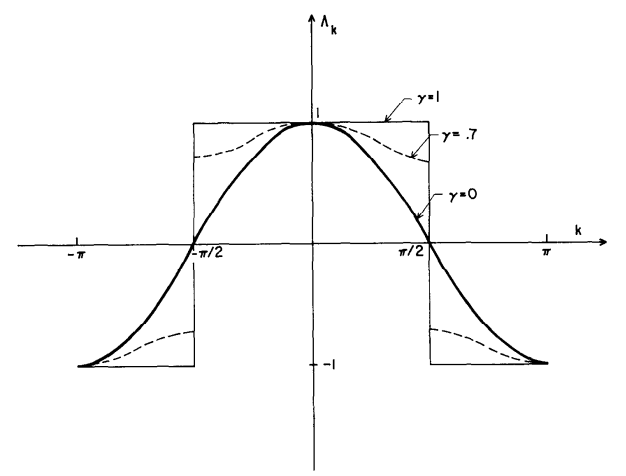
\includegraphics[scale=0.45]{figs/XY_HH_model/XY_S=0.5_HH_model_energies.png}}}
    \qquad
    \subfloat[\centering ]{{\includegraphics[scale=0.45]{figs/XY_HH_model/XY_excitation_spectrum.png}}}
    \caption{Fig. A: Energies of the elementary excitations in the $\textnormal{XY}_{S=\frac{1}{2}}$ Heisenberg model, as function of the wave vector for three different degrees of anisotropy. Retrieved from \cite{LIEB1961407}. Fig. B: Excitation spectra for the XY model for different anisotropy values $\gamma$. The \textcolor{red}{red} curve corresponds to the isotropic case $\gamma = 0$ - where the spectrum is gapless - and the \textcolor{blue}{blue} curve corresponds to the anisotropic case of $\gamma = 0.2$, where a gap appears.}
    \label{fig:XY_S=0.5_HH_model_energies} 
\end{figure}

Consider $N$ such that $\frac{N}{4} \notin \mathds{Z}$, hence $\Lambda_k \neq 0$. The sign of $\Lambda_k$ is arbitrary and can be taken to be positive. This corresponds to a particle-hole picture for the $\eta$-particles, where the ground states has no elementary fermions and the fermion excitations, both above and below the Fermi surface,\footnote{\begin{tcolorbox}[colback = yellow, title = Physical Context]

The Fermi surface consists of two points, $k = \frac{\pi}{2}$. The alternate picture in which all excitations are particles, which in the isotropic case is an up-spin $\ket{\uparrow}$, can be obtained by letting $\Lambda_k$ have the sign of $\Lambda_k$. The Fermi sea would then be defined by $|k| > \frac{\pi}{2}.$ However, the particle-hole picture is preferred. 

\end{tcolorbox}} have positive energies. The energy excitations for this model can be visualized in \cref{fig:XY_S=0.5_HH_model_energies}-(a). Only in the isotropic case $(\gamma = 0)$ there is no energy gap.\\

The ground state is defined as the state with no elementary excitations, thus 

\begin{equation}
\begin{array}{cc}
     \eta_{k} \ket{\Phi_0} = 0, \blanky \forall k.  \\
     E_0 = -\frac{1}{2} \sum_{k} \Lambda_k,
     \label{XY_ccyclic_gs}
\end{array}
\end{equation}

where $E_0$ is the ground-state energy. Notice that the ground state has zero total spin. This zero-total-spin ground state is non-degenerate, which is the same result as in the full Heisenberg model. 
In the thermodynamic limit, the preceding sum can be replaced by an integral, yielding 

\begin{equation}
    \begin{split}
    \frac{E_0}{N} =& -\frac{1}{4\pi} \int_{-\pi}^{\pi} dk \blanky \bigg[1 - (1-\gamma^2) \sin k \bigg] \\
    &= - \frac{1}{\pi} \mathcal{E}(1-\gamma^2),
    \begin{array}{cc}
         \textnormal{ which yields the  }  \\
         \textnormal{ following limiting cases }
    \end{array} \begin{array}{cc}
     \frac{E_0}{N} = - \frac{1}{\pi} & \textnormal{ for the isotropic case, } \gamma = 0\\ 
     \\
     \frac{E_0}{N} = - \frac{1}{2} & \textnormal{ for the Ising case, } \gamma = 1. 
\end{array}
    \end{split} 
\end{equation} 

where $\mathcal{E}(\cdot)$ is one of the complete elliptic integrals. The $\frac{E_0}{N}$-quantity is analytic and goes smoothly between the $(\gamma=0)$- and $(\gamma=1)$-limiting cases. In the thermodynamic limit $N \rightarrow \infty$, there are always gapless excitations near $k = \pm \frac{\pi}{2}$. These have a dispersion, $k = \pm \frac{\pi}{2} + q$, $\Lambda_k = |\sin q| \approx q$ as $q \rightarrow 0$. In \cref{fig:XY_S=0.5_HH_model_energies}-(b) plots of the excitation spectra are shown for different values of $\gamma$. \\

\begin{tcolorbox}[colback = yellow, title = Physical Context]

The previous relations hold, in principle, only or the $c$-cyclic problem, rather than the full $a$-problem. The Hamiltonian in the $a$-cyclic term has an additional non-local term 

$$
 - \frac{1}{2} \bigg[{\bf c}_N^\dagger {\bf c}_1 + {\bf c}_1^\dagger {\bf c}_N + \gamma {\bf c}_N^\dagger {\bf c}_1^\dagger + \gamma {\bf c}_1 {\bf c}_N\bigg] (e^{i\pi \mathfrak{F}} + 1).
$$

The $\mathfrak{F}$ is not invariant under the transformations shown in \cref{XY_Jordan_Wigner}, but its evenness or oddness does remain invariant, with the same being true for $e^{i\pi \mathfrak{F}}$. 

\begin{itemize}
    \item Now, in the ground state of the $c$-cyclic problem, given by \cref{XY_ccyclic_gs}, and in all states with an even number of excitations, the number of $c$-particles is odd (check the definition of the $c$-particles in terms of the $\eta$-particles, given by \cref{XY_Hamiltonian_diag_ops}, and consider that the ground state is defined in terms of the $\eta$-particles)\footnote{assuming $\frac{N}{4} \notin \mathds{Z}$, the $k$s are occupied symmetrically around $K = 0$, except that $k = \pi$, but no $k= -\pi$, is occupied. }. Hence an additional term gives zero net difference, when acting on said states and thus, for an even number of excitations, these states remain eigenstates of the $a$-cyclic problem. \\
    \item For states with an odd number of excitations, on the other hand, $\mathfrak{F}$ is even, giving rise to an additional term, 
    
    $$
        - \frac{1}{2} \bigg({\bf c}_N^\dagger {\bf c}_1+ \gamma {\bf c}_N^\dagger{\bf c}_1 + \textnormal{h.c.} \bigg),
    $$
    
    in the Hamiltonian. This induces corrections of $\mathcal{O}(N^{-1})$ on the $k$s, the $\bm{\Phi}_k$'s and the $\bm{\Psi}_k$'s, all of which can be calculated exactly but are negligible in the calculation of physical quantities. Strictly speaking, the elementary excitations are not independent for the $a$-cyclic problem, since there is a dependence on the evenness or oddness of the total number of excitations present. 
\end{itemize}

\end{tcolorbox}

\blanky \\

The free energy is given by the grand potential of such a system of non-interacting fermions with zero chemical potential,

\begin{equation}
    \frac{F_{\gamma}}{N} = -\beta^{-1} \bigg[\alpha + \frac{2}{\pi} \int_{0}^{\frac{\pi}{2}}\ dk \blanky \log \cosh \frac{\beta \Lambda_k}{2} \bigg], \begin{array}{cc}
         \textnormal{ which yields the  }  \\
         \textnormal{ following limiting cases }
    \end{array} \begin{array}{cc}
      \frac{F_{\textnormal{isotrop.}}}{N} = -\beta^{-1} \bigg[\alpha + \frac{2}{\pi} \int_{0}^{\frac{\pi}{2}}\ dk \blanky \log \cosh \frac{\beta \cos k}{2} \bigg] & \textnormal{ for the isotropic case, } \gamma = 0\\ 
     \\
      \frac{F_{\textnormal{isotrop.}}}{N} = - \frac{\alpha + \log \cosh \frac{\beta}{2}}{\beta} & \textnormal{ for the Ising case, } \gamma = 1,
\end{array},
\end{equation}

where $\alpha = \log 2$. Neither case exhibits any singular behaviour as a function of the temperature, a result to be expected in view of the one-dimensional nature of the model. \\

\begin{itemize}
    \item Antiferromagnetic case, isotropic case:
\end{itemize}

In the isotropic case, the mathematical treatment is simpler than that of the general anisotropic case. Since some of the eigenenergies will be negative, it is convenient to introduce an additional transformation, which reads

\begin{equation} 
 \begin{split}
      \begin{array}{cc}
         \bm{\zeta}_k = \eta_k & \textnormal{ if } \Lambda_{k} \geq 0,\\
         \bm{\zeta}_k = -\eta_k & \textnormal{ if } \Lambda_{k} < 0.
    \end{array} \Rightarrow {\bf H}_c =& \sum_{k, \Lambda_k \geq 0} \Lambda_k \bm{\zeta}_k^\dagger \bm{\zeta}_k + \sum_{k, \Lambda_k < 0} \Lambda_k \bm{\zeta}_k\bm{\zeta}_k^\dagger \\
    &= \sum_{k} |\Lambda_k| \bm{\zeta}_k^\dagger \bm{\zeta}_k - \sum_{k, \Lambda_k < 0} |\Lambda_k| \\
    &= \sum_{k} |\Lambda_k| \bigg( \bm{\zeta}_k^\dagger \bm{\zeta}_k - \frac{1}{2} \bigg),
 \end{split}
\end{equation}

where $\Tr {\bf A} = \sum_{k} \Lambda_k = 0$ was used. Here, the $\bm{\zeta}_k$-particles are fermionic in nature, thus the ground state satisfies $\bm{\zeta}_k\ket{0} = 0, \quad \forall k$, with the $\bm{\zeta}_k^\dagger$-operator generating elementary fermionic excitations with $|Lambda_k|$-energy above the ground state. Using translational invariance, the eigenvectors and eigenvalues of the ${\mathcal{A}}$-matrix are 

\begin{equation}
    \phi_{kj} = \frac{1}{\sqrt{N}} e^{ikj}, \blanky \Lambda_k = \cos k, \textnormal{ with } k = \frac{2\pi n}{N} \textnormal{ for } -\frac{N}{2} \leq n \leq \frac{N}{2} - 1.
\end{equation}

Hence, in the thermodynamic limit $N\rightarrow \infty$ there are always gapless excitations near the Fermi sphere, $k = \pm \frac{\pi}{2}$. These have a dispersion $k = \pm \frac{\pi}{2} + q$ with $\epsilon(k) = |\sin q| \approx |q|$ as $q \rightarrow 0$. The ground state energy per spin becomes 

\begin{equation*}
    \frac{U}{N} = - \frac{1}{N} \sum_{k} \frac{|\Lambda_k|}{2} \rightarrow -\int_{-\pi}^{\pi} \frac{dk}{4\pi} |\cos k| = - \frac{1}{\pi}.
\end{equation*}

Consider the $(N \in 2\mathds{N} \blanky \land \blanky \frac{N}{4} \notin \mathds{Z})$-case, so that the ground state is non-degenerate. In said case, the ground state of ${\bf H}_c$ is an exact eigenstate of ${\bf H}$ with the same eigenvalue. At any rate, the ground state is - at most - four-times degenerate. Then, the ground state spin properties read 

\begin{equation}
    \begin{split}
        &\spin^z = \sum_{i} {\bf c}_i^\dagger {\bf c}_i - \frac{N}{2} = \sum_{k} \eta_k^\dagger \eta_k - \frac{N}{2} = \sum_{k, \Lambda_k \geq 0} \bm{\zeta}_k^\dagger \bm{\zeta}_k + \sum_{k, \Lambda_k < 0} \bm{\zeta}_k\bm{\zeta}_k^\dagger - \frac{N}{2} \\
        &= \sum_{k, \Lambda_k \geq 0} \bm{\zeta}_k^\dagger \bm{\zeta}_k + \sum_{k, \Lambda_k < 0} (1- \bm{\zeta}_k^\dagger\bm{\zeta}_k) - \frac{N}{2} \\
        &= \sum_{k} \textnormal{sgn}(\Lambda_k) \bm{\zeta}_k^\dagger\bm{\zeta}_k + \sum_{k, \Lambda_k < 0} 1 - \frac{N}{2}
    \end{split}
\end{equation}

Thus, for excitations with $|k| < \frac{\pi}{2}$ carry $\spin^z = 1$ and for excitations with $|k| > \frac{\pi}{2}$ carry $\spin^z = -1$ 

\begin{equation}
    \begin{split}
        \Rightarrow \begin{array}{cc}
             \textnormal{ The total spin of the ground state is } \spin^z \ket{\Omega} = \bigg(\sum_{k, \Lambda_k < 0} 1-\frac{N}{2}\bigg) \ket{\Omega} = 0,
        \end{array} 
    \end{split}
\end{equation}

ie. the ground state is non-degenerate and carries zero total spin, as in the full Heisenberg model. \\

\begin{itemize}
    \item Ferromagnetic case
\end{itemize}

The previous results can be trivially generalized to the case of ferromagnetic coupling, wherein the Hamiltonian reads 

\begin{equation}
    {\bf H}_{\textnormal{ferro}} = - {\bf H} \approx -{\bf H}_c = \sum_{k} -|\Lambda_k| \bigg( \bm{\zeta}_k^\dagger \bm{\zeta}_k - \frac{1}{2} \bigg) = \sum_{k} |\Lambda_k| \bigg( \bm{\zeta}_k\bm{\zeta}_k^\dagger - \frac{1}{2} \bigg).
\end{equation}

Notice that the new, ferromagnetic, ground state now satisfies $\bm{\zeta}_k^\dagger \ket{0_F} = 0, \quad \forall k$. Hence, the ferromagnetic ground state can be obtained from the antiferromagnetic ground state by turning on all excitations, and the ferromagnetic excitations are obtained by removing the antiferromagnetic ones. In particular, the ground state energy and the excitation spectrum are the same as in the ferromagnetic case. The ground state is still non-degenerate and has zero total spin. 

\begin{equation}
    \begin{split}
        \spin^z \ket{0_F}=& \bigg( \sum_{k} \textnormal{sgn}(\Lambda_k) \bm{\zeta}_k^\dagger\bm{\zeta}_k + \sum_{k, \Lambda_k < 0} 1 - \frac{N}{2}\bigg) \ket{0_F} = \bigg( \sum_{k} \textnormal{sgn}(\Lambda_k) \bm{\zeta}_k^\dagger\bm{\zeta}_k + \sum_{k, \Lambda_k < 0} 1 - \frac{N}{2} \bigg)\ket{0_F} \\
        &= \bigg(\sum_{k, \Lambda_k \geq 0} 1 - \frac{N}{2}\ket{0_F} \bigg) = 0.
    \end{split}
\end{equation}

This is in clear contrast to the full ferromagnetic Heisenberg model, where the ground state is greatly degenerate, with one of the ground states carrying $\spin^z = \frac{N}{2}$. \\

\paragraph{\textswab{Short- and long-range order in the Ground state}} 

The long-range order for the Heisenberg model is often defined in terms of two sublattices\footnote{In the case of a linear one-dimensional chain, these sublattices may be defined to be, one corresponding to all even sites and the other one corresponding to all odd sites.}. It is taken to be the preponderance of spins up to spins down on one of the sublattices or viceversa.

\begin{tcolorbox}[colback = yellow, title = Physical Context]

For the $(\gamma=1)$-case, the ground state has long range Néel order, ie. $\spin^x_i \ket{\Psi_0} = (-1)^i \ket{\Psi_0}$ for the antiferromagnetic case, while in the ferromagnetic case $\spin^x_i \ket{\Psi_0} = \ket{\Psi_0}$. Therefore it is interesting to understand what happens in the intermediate values of $\gamma$. It is clear that states with spin-$x$- and spin-$y$-ordered components start to compete, yet it is not obvious whether the ground state has any long and/or short range order at $\gamma = 0$.

\end{tcolorbox}

\begin{itemize}
    \item Since the Heisenberg Hamiltonian is $SU(2)$-invariant, in particular it is invariant under a rotation in $\theta^{i} = \pi, \blanky i =x,y,z$,
    \item is translationally invariant,
    \item and the ground state is non-degenerate,
\end{itemize}

then, according to this definition for long-range order, it must be zero even if the state itself was ordered. However note that the completely ferromagnetic states can have long-range order by this definition only because these are highly degenerate. This definition for long-range order, though somewhat lacking, is useful since the approximate states considered have not always had the full symmetries of the Hamiltonian.\\

A much better measure for the long-range order is the time dependent dynamical spin correlation tensor, 

\begin{equation}
    \bm{\mathcal{S}}^{mn}(t) = \bra{\Psi_0} \spin_{n}(0) \spin_{m}(t) \ket{\Psi_0} \rightarrow \mathcal{S}^{mn} = \bra{\Psi_0} \spin_{n}(0) \spin_{m} \ket{\Psi_0},
\end{equation}

where the second expression is the $(t=0)$-contraction of the dynamical spin correlation tensor, which enters in the calculation of any process conceived to directly measure order. Then, 

\begin{equation}
    \begin{split}
        \mathcal{S}_{nm}^x = \bra{\Psi_0} \spin_n^x \spin_m^x \ket{\Psi_0} =& \frac{1}{4} \bra{\Psi_0} ({\bf a}_n^\dagger + {\bf a}_n)({\bf a}_m^\dagger + {\bf a}_m) \ket{\Psi_0}\\
            &= \frac{1}{4} \bra{\Psi_0} \bigg({\bf c}_n^\dagger e^{-i\pi \sum_{j = 1}^{n-1} {\bf c}_j^\dagger {\bf c}_j} + {\bf c}_n e^{i\pi \sum_{j = 1}^{n-1} {\bf c}_j^\dagger {\bf c}_j}\bigg) \bigg({\bf c}_m^\dagger e^{-i\pi \sum_{j = 1}^{m-1} {\bf c}_j^\dagger {\bf c}_j} + {\bf c}_m e^{i\pi \sum_{j = 1}^{m-1} {\bf c}_j^\dagger {\bf c}_j} \bigg)\ket{\Psi_0} \\
            &= \frac{1}{4} \bra{\Psi_0} \bigg({\bf c}_n^\dagger + {\bf c}_n e^{2i\pi \sum_{j = 1}^{n-1} {\bf c}_j^\dagger {\bf c}_j} \bigg) e^{-i\pi \sum_{j = 1}^{n-1} {\bf c}_j^\dagger {\bf c}_j} e^{i\pi \sum_{j = 1}^{m-1} {\bf c}_j^\dagger {\bf c}_j} \bigg({\bf c}_m^\dagger e^{-2i\pi \sum_{j = 1}^{n-1} {\bf c}_j^\dagger {\bf c}_j} + {\bf c}_m \bigg)\ket{\Psi_0}\\
            &= \frac{1}{4} \bra{\Psi_0} \bigg({\bf c}_n^\dagger + {\bf c}_n\bigg) e^{i\pi \sum_{j = n}^{m-1} {\bf c}_j^\dagger {\bf c}_j} \bigg({\bf c}_m^\dagger + {\bf c}_m \bigg)\ket{\Psi_0}\\
            &= \frac{1}{4} \bra{\Psi_0} \bigg({\bf c}_n^\dagger + {\bf c}_n\bigg) \prod_{j=n}^{m-1} ({1-2{\bf c}_j^\dagger {\bf c}_j}) \bigg({\bf c}_m^\dagger + {\bf c}_m \bigg)\ket{\Psi_0} \\
            &= \frac{1}{4} \bra{\Psi_0} \bigg({\bf c}_n^\dagger + {\bf c}_n\bigg) ({1-2{\bf c}_n^\dagger {\bf c}_n}) \prod_{j=n+1}^{m-1} ({1-2{\bf c}_j^\dagger {\bf c}_j}) \bigg({\bf c}_m^\dagger + {\bf c}_m \bigg)\ket{\Psi_0} \\
            &= \frac{1}{4} \bra{\Psi_0} \bigg({\bf c}_n^\dagger - {\bf c}_n\bigg) \prod_{j=n+1}^{m-1} ({\bf c}_j^\dagger + {\bf c}_j)({\bf c}_j^\dagger - {\bf c}_j) \bigg({\bf c}_m^\dagger + {\bf c}_m. \bigg)\ket{\Psi_0}.
    \end{split}
\end{equation}

Now, let ${\bf A}_n = {\bf c}_n^\dagger + {\bf c}_n$ and ${\bf B}_n = {\bf c}_n^\dagger - {\bf c}_n$, such that 

\begin{equation} \begin{split}
    \begin{array}{c}
         {\bf A}_n = {\bf c}_n^\dagger + {\bf c}_n  \\
         {\bf B}_n = {\bf c}_n^\dagger - {\bf c}_n 
    \end{array} \Rightarrow \begin{array}{c}
         \{{\bf A}_n, {\bf A}_m\} = \delta_{ij} \\
         \{{\bf B}_n, {\bf B}_m\} = -2\delta_{ij} \\
         \{{\bf A}_n, {\bf B}_m\} = 0 
    \end{array} \Longrightarrow
    \mathcal{S}_{nm}^x =& \frac{1}{4} \bra{\Psi_0} \bigg({\bf c}_n^\dagger - {\bf c}_n\bigg) \prod_{j=n+1}^{m-1} ({\bf c}_j^\dagger + {\bf c}_j)({\bf c}_j^\dagger - {\bf c}_j) \bigg({\bf c}_m^\dagger + {\bf c}_m. \bigg)\ket{\Psi_0} \\
         &= \frac{1}{4} \bra{\Psi_0} {{\bf B}}_n \prod_{j=n+1}^{m-1} {{\bf A}}_n {{\bf B}}_n {{\bf A}}_m \ket{\Psi_0}    \\
         &= \frac{1}{4} \bra{\Psi_0} {{\bf B}}_n {{\bf A}}_{n+1} {{\bf B}}_{n+1} {{\bf A}}_{n+2} \cdots {{\bf A}}_{m-1} {{\bf B}}_{m-1} {{\bf A}}_m \ket{\Psi_0}
    \end{split} 
\end{equation}

Similarly, for the other two correlators 

\begin{equation}
    \begin{split}
        \mathcal{S}_{nm}^y = \bra{\Psi_0} \spin_n^y \spin_m^y \ket{\Psi_0} =& \frac{1}{4} \bra{\Psi_0} ({\bf a}_n^\dagger - {\bf a}_n)({\bf a}_m^\dagger - {\bf a}_m) \ket{\Psi_0}\\
        &= \frac{1}{4} \bra{\Psi_0} \bigg({\bf c}_n^\dagger e^{-i\pi \sum_{j = 1}^{n-1} {\bf c}_j^\dagger {\bf c}_j} - {\bf c}_n e^{i\pi \sum_{j = 1}^{n-1} {\bf c}_j^\dagger {\bf c}_j}\bigg) \bigg({\bf c}_m^\dagger e^{-i\pi \sum_{j = 1}^{m-1} {\bf c}_j^\dagger {\bf c}_j} - {\bf c}_m e^{i\pi \sum_{j = 1}^{m-1} {\bf c}_j^\dagger {\bf c}_j} \bigg)\ket{\Psi_0} \\
            &= \frac{1}{4} \bra{\Psi_0} \bigg({\bf c}_n^\dagger - {\bf c}_n e^{2i\pi \sum_{j = 1}^{n-1} {\bf c}_j^\dagger {\bf c}_j} \bigg) e^{-i\pi \sum_{j = 1}^{n-1} {\bf c}_j^\dagger {\bf c}_j} e^{i\pi \sum_{j = 1}^{m-1} {\bf c}_j^\dagger {\bf c}_j} \bigg({\bf c}_m^\dagger e^{-2i\pi \sum_{j = 1}^{n-1} {\bf c}_j^\dagger {\bf c}_j} - {\bf c}_m \bigg)\ket{\Psi_0}\\
            &= \frac{(-1)^{m-n}}{4} \bra{\Psi_0} \bigg({\bf c}_n^\dagger - {\bf c}_n\bigg) e^{i\pi \sum_{j = n}^{m-1} {\bf c}_j^\dagger {\bf c}_j} \bigg({\bf c}_m^\dagger - {\bf c}_m \bigg)\ket{\Psi_0}\\
            &= \frac{(-1)^{m-n}}{4} \bra{\Psi_0} \bigg({\bf c}_n^\dagger - {\bf c}_n\bigg) \prod_{j=n}^{m-1} ({1-2{\bf c}_j^\dagger {\bf c}_j}) \bigg({\bf c}_m^\dagger - {\bf c}_m \bigg)\ket{\Psi_0} \\
            &= \frac{(-1)^{m-n}}{4} \bra{\Psi_0} \bigg({\bf c}_n^\dagger - {\bf c}_n\bigg) ({1-2{\bf c}_n^\dagger {\bf c}_n}) \prod_{j=n+1}^{m-1} ({1-2{\bf c}_j^\dagger {\bf c}_j}) \bigg({\bf c}_m^\dagger - {\bf c}_m \bigg)\ket{\Psi_0} \\
            &= \frac{(-1)^{m-n}}{4} \bra{\Psi_0} \bigg({\bf c}_n^\dagger + {\bf c}_n\bigg) \prod_{j=n+1}^{m-1} ({\bf c}_j^\dagger - {\bf c}_j)({\bf c}_j^\dagger + {\bf c}_j) \bigg({\bf c}_m^\dagger - {\bf c}_m. \bigg)\ket{\Psi_0} \\
            &= \frac{(-1)^{m-n}}{4} \bra{\Psi_0} {{\bf A}}_n \prod_{j=n+1}^{m-1} {{\bf B}}_n {{\bf A}}_n {{\bf B}}_m \ket{\Psi_0}    \\
         &= \frac{(-1)^{m-n}}{4} \bra{\Psi_0} {{\bf A}}_n {{\bf B}}_{n+1} {{\bf A}}_{n+1} {{\bf B}}_{n+2} \cdots {{\bf B}}_{m-1} {{\bf A}}_{m-1} {{\bf B}}_m \ket{\Psi_0}
        \\
         \mathcal{S}_{nm}^z = \bra{\Psi_0} \spin_n^z \spin_m^z \ket{\Psi_0} =& \bra{\Psi_0} \bigg({\bf a}_n^\dagger {\bf a}_n - \frac{1}{2}\bigg) \bigg({\bf a}_m^\dagger {\bf a}_m - \frac{1}{2}\bigg)\ket{\Psi_0} = \frac{1}{4} \bra{\Psi_0} {{\bf A}}_i {{\bf B}}_i {{\bf B}}_i {{\bf A}}_i\ket{\Psi_0}.\\
    \end{split}
\end{equation}

These expressions may be evaluated using Wick's theorem, which allows to express the vacuum expectation value of a product of operators, all of which obey anticommutation rules, in terms of contractions of pairs. A particular simplification occurs in evaluating the previous set of expectation values. The basic contractions may be readily calculated, 

\begin{align}
    \langle {\bf A}_i {\bf A}_j \rangle &= \sum_{k} \phi_{ki} \phi_{kj} = \delta_{ij} & \langle {\bf B}_i {\bf B}_j \rangle &= -\sum_{k} \psi_{ki} \psi_{kj} = -\delta_{ij} & \langle {\bf B}_i {\bf A}_j \rangle \begin{array}{cc}
         = -\langle {\bf A}_j {\bf B}_i \rangle  \\
         = -\sum_{k} \phi_{ki} \psi_{kj} = \mathfrak{G}_{ij}
    \end{array}.
    \label{XY_aux_var_correlators}
 \end{align}

Thus, the most straightforward pairing contribution to $\mathcal{S}_{nm}^x$ is

\begin{equation}
    \langle {\bf B}_{n} {\bf A}_{n+1} \rangle \langle {\bf B}_{n+1} {\bf A}_{n+2} \rangle \cdots \langle {\bf B}_{m-1} {\bf A}_{m} \rangle,
\end{equation}

since all other pairings can be obtained from this one via permutations of the ${\bf A}$-operators, keeping the ${\bf B}$-operators fixed. Since the number of crossings of ${\bf B}$-operators by ${\bf A}$-operators is always even, the sign associated with a given permutation is $(-1)^{-\textnormal{sgn}(\sigma)}$, with $\textnormal{sgn}(\sigma)$ the signature of the permutation of the ${\bf A}$-operators. Thus, the following identities hold

\begin{equation}
    \begin{split}
        &\mathcal{S}_{nm}^x = \frac{1}{4} \sum_{\sigma \in \mathcal{S}[n+1,m]} (-1)^{\textnormal{sgn}(\sigma)} \mathfrak{G}_{n, \sigma(n+1)} \cdots \mathfrak{G}_{m-1, \sigma(m)} = \frac{1}{4} \left| \begin{array}{cccc}
          \mathfrak{G}_{n, n+1} & \mathfrak{G}_{n, n+2} & \cdot & \mathfrak{G}_{nm}  \\
          \vdots & & \vdots\\
          \mathfrak{G}_{m-1, n+1} & \mathfrak{G}_{m-1, n+2} & \cdot & \mathfrak{G}_{m-1, m}  \\
        \end{array} \right| \\
        &\mathcal{S}_{nm}^y = \frac{1}{4} \sum_{\sigma \in \mathcal{S}[n,m-1]} (-1)^{\textnormal{sgn}(\sigma)} \mathfrak{G}_{n+1, \sigma(n)} \cdots \mathfrak{G}_{m, \sigma(m-1)} = \frac{1}{4} \left| \begin{array}{cccc}
          \mathfrak{G}_{n+1, n} & \mathfrak{G}_{n+1, n+1} & \cdot & \mathfrak{G}_{n+1,m-1}  \\
          \vdots & & \vdots\\
          \mathfrak{G}_{m, n} & \mathfrak{G}_{m, n+2} & \cdot & \mathfrak{G}_{m, m-1}  \\
        \end{array} \right| \\
         &\mathcal{S}_{nm}^z = \frac{1}{4} \bigg(\langle {\bf A}_n {\bf B}_m\rangle \langle {\bf A}_m {\bf B}_m \rangle - \langle {\bf A}_n {\bf B}_m \rangle \langle {\bf B}_m {\bf A}_n \rangle \bigg) = \frac{1}{4} (\mathfrak{G}_{nn} \mathfrak{G}_{m,m} - \mathfrak{G}_{m, n} \mathfrak{G}_{n,m}), \textnormal{ for } n<m,
         \label{XY_correlators_matrices}
    \end{split}
\end{equation}

and where $\mathcal{S}[a,b]$ is the group of permutations of integers $\mathds{Z}_{[a,b]}$. Note that the first two submatrices of \cref{XY_correlators_matrices} can be written as 

\begin{equation*}
    \begin{array}{cc}
     \begin{split}
         (\mathcal{S}_{nm}^x)_{ij} =& \frac{1}{4} (\mathfrak{G}_{nm}^x)_{ij} \\
         &= \frac{1}{4} \mathfrak{G}_{n+i-1,j+n}
     \end{split} \quad 
     \begin{split}
         (\mathcal{S}_{nm}^y)_{ij} =& \frac{1}{4} (\mathfrak{G}_{nm}^y)_{ij} \\
         &= \frac{1}{4} \mathfrak{G}_{n+i, n+j-1}
     \end{split} 
\end{array}
\end{equation*}

Thus, both $\mathcal{S}_{nm}^x$ and $\mathcal{S}_{nm}^y$
 are particular subdeterminants of $\det \bm{\mathfrak{G}}$, where $\bm{\mathfrak{G}}$ is a matrix with entries 
 
 $$
    (\bm{\mathfrak{G}})_{ij} = - (c)_{ij}, \begin{array}{cc}
         \textnormal{ where $\bm{\Phi}$ are the matrices of ${\phi_{k,i}}$}  \\
         \textnormal{ where $\bm{\Psi}$ are the matrices of ${\psi_{k,i}}$}.
    \end{array}
 $$
 
It it obvious that this $\bm{\mathfrak{G}}$-matrix is unitary, since both $\bm{\Psi}$ and $\bm{\Phi}$ are unitary as well, and its determinant is then $\pm 1$. Its actual sign can be found to be $\det \bm{\mathfrak{G}} = 
(-1)^N \det \bm{\mathfrak{G}}$. \\

In order to calculate this Green function matrix, defined in \cref{XY_aux_var_correlators}, the thermodynamical limit is taken, yielding 

\begin{equation}
    \begin{split}
        \mathfrak{G}_{ij} =& - \sum_{k} \psi_{ki} \phi_{kj} = - \sum_{k} \frac{1}{\Lambda_k} \bigg(\phi_{ki} \cos k + \gamma \phi_{-k i} \sin k\bigg) \phi_{k,j} \\
        &= \frac{1 + (-1)^{i-j+1}}{2} \bigg(-\frac{2}{\pi}\bigg) \int_{0}^{\frac{\pi}{2}} dk \blanky \frac{1}{\Lambda_k} \bigg(\cos k \cos k(i-j) - \gamma \sin k \sin k(i-j\bigg),
    \end{split}
\end{equation}

where \cref{XY_psi_kj_coeffs} was used in the second equality in the first line. Notice that $\mathfrak{G}$ depends only on the difference $i-j$, a consequence of the cyclic-ness of the spin chain and its translational invariance. Hence, $\mathfrak{G}_{ij} = \mathfrak{G}_{i-j}$, being zero if $i-j$ is even. In the limiting cases, closed expressions can be obtained

\begin{equation}
    \begin{array}{cc}
        \mathfrak{G}_{ij} = \left\{ \begin{array}{cc}
            -\delta_{i-j, -1}  & \textnormal{ for } i-j \textnormal{ odd }\\
             0 & \textnormal{ for } i-j \textnormal{ even}
        \end{array} \right. & \textnormal{ in the isotropic limit, $\gamma = 0$,} \\
        \mathfrak{G}_{ij} = \left\{ \begin{array}{cc}
             (-1)^{\frac{i-j+1}{2}} \frac{2}{\pi (i-j)}   & \textnormal{ for } i-j \textnormal{ odd }\\
             0 & \textnormal{ for } i-j \textnormal{ even}
        \end{array} \right. & \textnormal{ in the Ising limit, $\gamma = 1$.} 
    \end{array}
\end{equation}

With these elements, the ground state order can be evaluated. In particular, the ground state correlations for the XY-model between nearest-neighbours at finite anisotropy, 

\begin{equation}
    \begin{split}
        &\mathcal{S}_1^x = \mathcal{S}^x_{i,i+1} = \frac{1}{4} \mathfrak{G}_{i,i+1} \equiv \frac{1}{4} \mathfrak{G}_{-1} \\
        &\mathcal{S}_1^y = \mathcal{S}^y_{i,i+1} = \frac{1}{4} \mathfrak{G}_{i+1,i} \equiv \frac{1}{4} \mathfrak{G}_{1} \textnormal{ where } \mathfrak{G}_{\pm1} = - \frac{2}{\pi} \frac{1}{1 \mp \gamma} \bigg(\mathcal{E}(\sqrt{1-\gamma^2}) \mp \gamma \mathcal{K}(\sqrt{1-\gamma^2})\bigg), \\
        &\mathcal{S}_1^z = \mathcal{S}^z_{i,i+1} = \frac{1}{4} \bigg(\mathfrak{G}_{i,i}\mathfrak{G}_{i+1,i+1} - \mathfrak{G}_{i,i+1}\mathfrak{G}_{i+1,i} \bigg)\equiv \frac{1}{4} \mathfrak{G}_{-1}\mathfrak{G}_{1}
    \end{split}, 
\end{equation}

\begin{figure}
    \centering
    \includegraphics[scale = .5]{figs/XY_HH_model/XY_NNcorrs_plot.png}
    \caption{Nearest-neighbour correlators plotted as function of the anisotropy $\gamma$, where, 
        the \textcolor{red}{red} curve corresponds to $\mathcal{S}_1^x$, 
        the \textcolor{blue}{blue} curve corresponds to $\mathcal{S}_1^y$,
        and where the \textcolor{green}{green} curve corresponds to $\mathcal{S}_1^z$.
    From these plots it is clear that the $x$- and $y$-correlations compete as $\gamma \rightarrow 0. $
    }
    \label{fig:XY_NN_corrs}
\end{figure}

where the elliptic E and K functions were introduced. These correlators are plotted in \cref{fig:XY_NN_corrs}. For any value of $\gamma$, all of these correlations are negative in value, and hence the nearest-neighbours display antiferromagnetic correlations. 

\begin{itemize}
    \item For the Ising limit, $\gamma = 1$, $\mathcal{S}_1^x = \frac{1}{4}$ and $\mathcal{S}_1^y = \mathcal{S}_1^z = 0$. 
    \item As $\gamma$ decreases, the antiferromagnetic correlation between the $y$-components induce an anti-ferromagnetic correlation between the $z$-components. 
    \item Finally, in the isotropic limit $\gamma=0$, the $x$- and $y$-correlations between nearest-neighbours spins become equal (as expected for symmetry reasons), and $\mathcal{S}_1^x = \mathcal{S}_1^y = -\frac{1}{2\pi}, \mathcal{S}_1^z = - \frac{1}{\pi^2}$. So, short-range order persists in the isotropic limit.
\end{itemize}

\clearpage

\paragraph{$\Delta \approx 1$\textswab{: The isotropic Heisenberg Antiferromagnet}}

The most interesting regime for the XXZ chain is $\Delta \approx 1$, ie. the vicinity of the Isotropic Heisenberg antiferromagnet (HAF), wherein the ground state energy is given by 

$$
    E_0 = - N J \log 2.
$$

\clearpage

\subsection{\underline{General considerations of the Heisenberg model}}

\subsubsection{\textit{Antiferromagnetic Ground States}}

Consider an $N$-lattice system with spin-$S$, with Hamiltonian

\begin{equation}
    {\bf H} = {\bf H}^{zz} + {\bf H}^{xy}, \begin{array}{c}
         {\bf H}^{zz} = \frac{1}{2} \sum_{ij \in \Lambda \subset Z^{d}} J_{ij} \spin_i^z \spin_j^z, \\  
         \\
         {\bf H}^{xy} = \frac{1}{4} \sum_{ij \in \Lambda \subset Z^{d}} J_{ij} (\spin_i^+ \spin_j^- + \spin_i^- \spin_j^+), \\  
    \end{array}
    \label{auerbach's HH hamiltonian}
\end{equation}

with $J_{ij} = J_{ji}$ having translational symmetry. Furthermore, this Hamiltonian is rotationally invariant, having an $SU(2)$-symmetry, since it commutes with all three components of the total spin. Thus, the eigenstates may be labelled as

\begin{equation}
    \begin{array}{c}
         \ket{\Phi} = \ket{\spin_{\textnormal{tot}}, M, \cdots},  \\
         M = -\spin_{\textnormal{tot}}, - -\spin_{\textnormal{tot}} +1, \cdots,  \spin_{\textnormal{tot}}, \\          \spin_{\textnormal{tot}} \leq NS, 
    \end{array} \begin{array}{c}
         \textnormal{ where $M$ is the eigenvalue of the total magnetization $\spin_{\textnormal{tot}}^z$,}
         \\
         \textnormal{ and where $\spin_{\textnormal{tot}}^2 = \spin_{\textnormal{tot}}(\spin_{\textnormal{tot}}+1)$ is the $SU(2)$-Casimir invariant. } \\
         \textnormal{Note that, if the model is translationally invariant} \\
         \textnormal{the ${\bf k}$-momentum is also a good quantum number.}
    \end{array}
\end{equation}

\blanky \\

The antiferromagnetic ground state is, in general, far more complicated than the ferromagnetic ground state. There are a series of theorems on the ground states, which hold for bipartite antiferromagnetic Hamiltonians. Consider two lattices, $A$ and $B$, then the staggered magnetization operator on these sublattices is given by 

\begin{equation}
    \spin^{\textnormal{stagg}} = \sum_{i \in A} \spin_{i}^z - \sum_{i \in B} \spin_{i}^z.
\end{equation}

The Ising configurations form the basis set 

\begin{align*}
&\prod_{i=1}^{N} \ket{S, m_{i}^\alpha}_{i}
     \textnormal{ where $\ket{S, m_i}_i$ is an eigenstate of $\spin_i^2, \spin_i^z$ with eigenvalues $S(S+1), m_i$ respectively.} \\
&\begin{array}{cc}
     \textnormal{In this bipartite system, the Néel state maximizes the staggered }  \\
     \textnormal{ magnetization $\spin^{\textnormal{stagg}}$ and is given by the Ising configuration} 
\end{array}
    \ket{\Psi^{\textnormal{{Néel}}}} = \prod_{i=1}^{N} \ket{S, \eta_i S_i}, \quad \eta_i = \left\{\begin{array}{cc}
        1 & i \in A  \\
        -1 & i \in B
    \end{array} \right.
\end{align*}

Generally, this state is not an eigenstate of the Hamiltonian, since the spin flip terms $\spin_i^+ \spin_j^-$ connect the Néel state to other (non-Néel) Ising spin configurations. Now, it is convenient to rotate the spin axes on the $B$-sublattice about the $z$-axis, which amounts to the unitary transformation 

\begin{equation}\begin{array}{c}
     \spin_i^+ \rightarrow - \tilde{\spin}_i^+ \\
     \spin_i^- \rightarrow - \tilde{\spin}_i^- \\
     \spin_i^z \rightarrow + \tilde{\spin}_i^z, 
\end{array}
    \ket{S, m_i}_i \rightarrow \ket{S, \tilde{m}_i}_i = \left\{\begin{array}{cc}
        \ket{S, m_i}_i & i \in A \\
        (1-)^{S+m_i} \ket{S, m_i}_i & i \in B 
    \end{array} \right., 
    \label{HH_su2_rotation}
\end{equation}

where $\tilde{m}_i$ are eigenvalues of $\spin_i^z$ and $\tilde{\spin}_i^z$ on $A$ and $B$ sublattices, respectively. By restricting the problem to an $M$-subspace, all wave functions may be rewritten as 

\begin{equation}
    \ket{\Psi^M} = \sum_{\alpha} f_{\alpha}^M \ket{\tilde{\Psi}^M_{\alpha}}, \textnormal{ where } \ket{\tilde{\Psi}^M_{\alpha}} = \prod_{\sum_{i} \tilde{m}_i^\alpha = M} \ket{S, \tilde{m}_i^\alpha}. 
\end{equation}

Then, the following theorems, first presented by Marshall and then extended by Lieb and Mattis, arise \\

\clearpage

%\begin{tcolorbox}[title = Marshall's theorems]

\begin{theorem}
    Consider the Hamiltonian \cref{auerbach's HH hamiltonian} of a bipartite lattice, with \textnormal{antiferromagnetic} exchanges $J_{ij} \geq 0$ which connect two sublattices $A$ and $B$. Said antiferromagnetic exchanges are such that any two lattice sites are connected by a sequence of finite exchanges between intermediary sites. In any allowed $M$-sector, the lowest energy state $\ket{\Psi^M_0}$ can be chosen to have positive-definite coefficients in the rotated Ising basis $\ket{\tilde{\Psi}^M_{\alpha}}$ ie.
    
    \begin{align}
        \ket{\Psi^M_0} &= \sum_{\alpha} f_{\alpha}^M \ket{\tilde{\Psi}^M_{\alpha}}, \quad\{f_{\alpha}^M\}_{\alpha} > 0.
    \end{align}
    
    Therefore, the coefficients of $\ket{\Psi^M_0}$, in terms of the unrotated Ising configurations $\ket{\Psi_\alpha}$ obey the \textnormal{\textcolor{red}{{Marshall sign criterion}}},
    
    \begin{equation}
        \ket{\Psi^M_0} = \sum_{\alpha} (-1)^{\Gamma(\alpha)} f_{\alpha}^M \ket{{\Psi}^M_{\alpha}}, \quad \Gamma(\alpha) = \sum_{i \in B} (S + m_i^\alpha).
    \end{equation}
    \label{Marshall_theo_1}
\end{theorem}

\begin{theorem}
The absolute ground state $\ket{\Omega}$, for equal size sublattices $A$ and $B$, is a singlet of zero total spin, this is 

$$
    {\spin}_{\textnormal{tot}} \ket{\Psi^M_0}= 0.
$$
\label{Marshall_theo_2}
\end{theorem}
%\end{tcolorbox}

Note that not all total singlets obey the so-called Marshal sign criterion and, conversely, not all Marshall sign-obeying states are singlets of the total spin. The ground state of the Heisenberg Hamiltonian must, however, obey both conditions. \\

\begin{proof}

Consider an $SU(2)$-rotation, acting trivially on the first lattice and non-trivially in the second system. This is,

$$
    U \in SU(2) | U: (\mathfrak{s}\mathfrak{u}(2)_A) \times (\mathfrak{s}\mathfrak{u}(2)_B) \rightarrow (\mathfrak{s}\mathfrak{u}(2)_A) \times (\mathfrak{s}\mathfrak{u}(2)_B) \blanky \land \blanky \begin{array}{cc}
        () &  \\
         & 
    \end{array}
$$

Consider an $SU(2)-$rotation, under which the spin operators and Ising basis transform as \cref{HH_su2_rotation}. The Heisenberg Hamiltonian in this new representation then reads 

\begin{equation}
\begin{split}
    & \tilde{{\bf H}} = \tilde{{\bf H}}^{zz} + \tilde{{\bf H}}^{xy}, \begin{array}{c}
        \tilde{{\bf H}}^{zz} = \sum_{ij \in \Lambda \subset Z^{d}} |J_{ij}| \spin_i^z \tilde{\spin}_j^z, \\  
         \\
        \tilde{{\bf H}}^{xy} = - \frac{1}{2} \sum_{ij \in \Lambda \subset Z^{d}} |J_{ij}| (\spin_i^+ \tilde{\spin}_j^- + \spin_i^- \tilde{\spin}_j^+), \\  
    \end{array} \\
    & \textnormal{wherein, in this new sublattice-rotated representation,} \\
    & \begin{array}{cc}
       \textnormal{the longitudinal term, $\tilde{{\bf H}}^{zz}$, is diagonal in the  } & \textnormal{ and where the transverse $\tilde{{\bf H}}^{xy}$ has non-positive } \\
        \textnormal{rotated Ising configuration: } \tilde{{\bf H}}^{zz}\ket{\tilde{\Psi}_{\alpha}} = e_{\alpha} \ket{\tilde{\Psi}_{\alpha}} & \textnormal{ matrix elements:} 
        \bra{\tilde{\Psi}_{\alpha}} \tilde{{\bf H}}^{xy}  \ket{\tilde{\Psi}_{\beta}} = -|K_{\alpha \beta}|.
    \end{array}
    \label{auerbach's HH hamiltonian}
\end{split}
\end{equation}

Both of these matrix representations induce the following eigenvalue equation on the $f$-coefficients, 

\begin{equation*}\begin{split}
    \tilde{{\bf H}} \ket{\tilde{\Psi}_{\alpha}} = E \ket{\tilde{\Psi}_{\alpha}} \Rightarrow - \sum_{\beta} |K_{\alpha \beta}| f_{\beta} + e_{\alpha} f_{\alpha} = E f_{\alpha}. \\
    \textnormal{Consider then the trial function
          $\ket{\tilde{\Omega}} = \sum_{\alpha} |f_{\alpha}| \ket{\tilde{\Psi}_{\alpha}}$}      \textnormal{ whose energy is }
    \bra{\tilde{\Omega}} \tilde{{\bf H}} \ket{\tilde{\Omega}} &=  \sum_{\alpha} e_{\alpha} |f_{\alpha}|^2 - \sum_{\alpha \beta} |K_{\alpha \beta}| |f_{\alpha}| |f_{\beta}| \\
    & \leq \sum_{\alpha} e_{\alpha} |f_{\alpha}|^2 - \sum_{\alpha \beta} |K_{\alpha \beta}| f_{\alpha} f_{\beta} = E,
\end{split}
\end{equation*}

where the last equality holds if and only if all of the $f_{\alpha}$-coefficients are non-negative or all of the $f_{\alpha}$-coefficients are negative. This state must, therefore, also be a ground state and satisfy the eigenvalue equation 

$$
    - \sum_{\beta} |K_{\alpha \beta}| |f_{\beta}| + e_{\alpha} |f_{\alpha}| = E |f_{\alpha}|.
$$

In general, the $\ket{\tilde{\Psi}}$-states are not eigenstates of the rotated Hamiltonian, except in the case in which $M = NS$ which is the case of a one-state space. Therefore, $e_{\alpha} > E, \blanky \forall \alpha$. Then, 

\begin{equation}
    \begin{split}
    &(e_{\alpha} - E) f_{\alpha }= \sum_{\beta} |K_{\alpha \beta}| f_\beta \\
    &(e_{\alpha} - E) |f_{\alpha}|= \sum_{\beta} |K_{\alpha \beta}| |f_\beta|  
    \end{split} \Rightarrow \bigg|\sum_{\beta} |K_{\alpha \beta}| f_{\beta}\bigg| = \sum_{\beta} |K_{\alpha \beta}| |f_{\beta}| \Rightarrow f_{\beta} \geq 0.
\end{equation}

Thus, the trial state and the ground states are the same, upto phase factors: $\ket{\tilde{\Omega}} = \pm \ket{\Psi^M_0}$. An even stronger condition on the $f_{\beta}$s can be imposed.

\begin{lemma}
   $f_{\beta} > 0, \blanky \forall \beta$.
\end{lemma}

\begin{proof}
In effect, any Ising configuration with total magnetization $M$ is connected to all other configurations in the same sector by successive application of the pairwise spin flip operator ${\bf K}_{\alpha \beta} \approx (\sum_{i,j} \spin_i^+ \tilde{\spin}_j^- + \spin_i^- \tilde{\spin}_j^+)_{\alpha \beta}$. Thus, if $\exists \alpha: f_{\alpha} = 0$ , then $f_{\beta}$ must vanish for all other $\beta$ in the same $M$-sector. Since, by design, the ground state is such that in its expansions there is at least one non-zero coefficient, it follows that $f_{\beta} > 0$, $\forall{\beta}$, thus proving \cref{Marshall_theo_1}.
\end{proof}

\begin{corr}
For any fixed $M$, $\ket{\Psi^M_0}$ is non-degenerate.
\label{HH_non_degeneracy}
\end{corr}

\begin{proof}
In effect, since all $f_{\beta}$s are non-zero, there cannot be an orthogonal state to $\ket{\Omega}$ that has only positive definite coefficients in said $M$ subspace. \\
\end{proof}

For \cref{Marshall_theo_2} to hold, the ground state of the $M$-sector must have minimally possible total spin, 

\begin{lemma}
   For a bipartite antiferromagnetic Heisenberg model, 
   
   $$
   (\spin_{\textnormal{tot}})^2 \ket{\Psi^M} = M(M+1)\ket{\Psi^M}
   $$
\end{lemma}

\begin{proof}
Consider the infinite range Hamiltonian on a bipartite lattice with equal number of sites on the two sublattices, 

$$
    {\bf H}^{\infty} = J \sum_{\substack{
    i \in A \\
    j \in B}} \vec{\spin}_i \cdot \vec{\spin}_j = J \spin_{\textnormal{tot}}^A \cdot \spin_{\textnormal{tot}}^B
$$

This problem is thus trivially solvable, since it is a two spin problem using $\spin_{\textnormal{tot}} = \spin_{\textnormal{tot}}^A + \spin_{\textnormal{tot}}^B$, since $\spin_{\textnormal{tot}}^A \cdot \spin_{\textnormal{tot}}^B = \frac{1}{2} \bigg( \spin_{\textnormal{tot}}^2 - (\spin_{\textnormal{tot}}^A)^2 - (\spin_{\textnormal{tot}}^B)^2 \bigg)$.
Therefore, the possible values of the total spin operators are 

$$
    \spin_{\textnormal{tot}}^A, \spin_{\textnormal{tot}}^B = 0, 1, \cdots, \frac{NS}{2},
$$

which for equal size sublattice means that 

\begin{equation}
    0 \leq \spin_{\textnormal{tot}} \leq NS.
    \label{infinite_range_HH_total_spin}
\end{equation}

This infinite-range Hamiltonian's eigenvalues are then 

\begin{equation}
    E^{\infty} (\spin_{\textnormal{tot}}) = \frac{J}{2} \bigg[\spin_{\textnormal{tot}}(\spin_{\textnormal{tot}} + 1) - \spin_{\textnormal{tot}}^A(\spin_{\textnormal{tot}}^A+1) - \spin_{\textnormal{tot}}^B(\spin_{\textnormal{tot}}^B)\bigg],
\end{equation}

which are monotonically increasing with $\spin_{\textnormal{tot}}$, and since $\spin_{\textnormal{tot}} > M$, the ground state in a given $M$-sector has 

$$
\spin_{\textnormal{tot}} = M.
$$

Now, note that both the Heisenberg Hamiltonian and the infinite range Hamiltonian satisfy the requirements for the first of Marshall's theorems, \cref{Marshall_theo_1}, and thus their ground states have Marshall signs. Therefore, their overlap is non-zero, since it involves a sum over positive number, and these must have the same total spin quantum numbers. Therefore, the lowest energy state of ${\bf H}$ in the $M$-sector has spin $\spin_{\textnormal{tot}} = M$. Since all allowed values of total spin $\spin_{\textnormal{tot}}' > M$ have members in the sector with magnetization $M$, then the energy in terms of the total spin obeys 

$$
    \forall \spin_{\textnormal{tot}}' > \spin_{\textnormal{tot}} \Rightarrow E(\spin_{\textnormal{tot}}') > E(\spin_{\textnormal{tot}}),
$$

ie. the energy is a monotonically increasing function of the total spin. Now, consider the $(M=0)$-sector. This inequality proves that the ground state must have minimal possible total spin $\spin_{\textnormal{tot}}$ which is zero, according to \cref{infinite_range_HH_total_spin}. Thus concluding the proof of \cref{Marshall_theo_2}.
\end{proof}
\end{proof}

\subsubsection{\textit{Ferromagnetic Ground States}}

For the ferromagnetic Heisenberg chains, a similar result can be proved. 

\begin{corr}
\label{Ferromagnetic_Marshall_theo}
For the ferromagnetic model with non-positive charges, 

$$
{\bf H} = - \frac{1}{2} \sum_{ij} |J_{ij}| \vec{\spin}_i \cdot \vec{\spin}_j,
$$

the fully ferromagnetic state $\ket{\Psi^{\textnormal{FM}}}$ is a member of the ground state multiplet, where 

$$
    \ket{\Psi^{\textnormal{FM}}} = \prod_{i=1}^N \ket{S, S}_i.
$$

\end{corr}

\begin{proof}

Consider the ferromagnetic Heisenberg model, whose Hamiltonian may be explicitly written as 

\begin{equation}
     {\bf H} = {\bf H}^{zz} + {\bf H}^{xy}, \begin{array}{c}
         {\bf H}^{zz} = -\frac{1}{2} \sum_{ij \in \Lambda \subset \mathds{Z}^{2}} |J_{ij}| \spin_i^z \spin_j^z, \\  
         \\
         {\bf H}^{xy} = -\frac{1}{4} \sum_{ij \in \Lambda \subset \mathds{Z}^{2}} |J_{ij}| (\spin_i^+ \spin_j^- + \spin_i^- \spin_j^+). \\  
    \end{array}
\end{equation}

For a fixed $M$-subspace, all wave functions may be written in terms of Ising configurations which lie in said $M$-subspace, namely

\begin{equation}
    \ket{\Psi^M} = \sum_{\alpha} f_{\alpha}^M \ket{{\Psi}^M_{\alpha}}, \textnormal{ where } \ket{{\Psi}^M_{\alpha}} = \prod_{\sum_{i} {m}_i^\alpha = M} \ket{S, {m}_i^\alpha}. 
\end{equation}

Now, 

\begin{itemize}
    \item the longitudinal term, ${{\bf H}}^{zz}$, is diagonal in the Ising configurations, ${{\bf H}}^{zz}\ket{{\Psi}_{\alpha}} = e_{\alpha} \ket{{\Psi}_{\alpha}}$,
    \item and where the transverse ${{\bf H}}^{xy}$ has non-negative $\bra{{\Psi}_{\alpha}} {{\bf H}}^{xy}  \ket{{\Psi}_{\beta}} = |K_{\alpha \beta}|$.
\end{itemize}

Consider the following ansatz, $\ket{\Omega} = \sum_{\alpha} |f_{\alpha}| \ket{\Psi}_{\alpha}$, whose energy is 

\begin{equation}
\begin{split}
    \bra{\Omega} H \ket{\Omega} = & \sum_{\alpha} e_{\alpha} |f_{\alpha}|^2 + \sum_{\alpha \beta} |K_{\alpha \beta}| |f_{\alpha}| |f_{\beta}| \\
    & \leq \sum_{\alpha} e_{\alpha} |f_{\alpha}|^2 + \sum_{\alpha \beta} |K_{\alpha \beta}| f_{\alpha} f_{\beta} = E \Rightarrow \textnormal{sgn}(f_{\alpha}) = \textnormal{sgn}(f_{\beta}), \forall \alpha, \beta. 
\end{split}
\end{equation}

Without loss of generality, the $f_{\alpha}$-coefficients may be taken to be positive, with the extra, overall, sign to be associated with the Ising configurations. In effect, in general, the $\ket{{\Psi}}$-states are not  eigenstates of the Hamiltonian, except in the case in which $M = NS$ which is the case of a one-state space. Therefore, $e_{\alpha} > E, \blanky \forall \alpha$.
Consider the infinite range ferromagnetic Hamiltonian on a bipartite lattice with equal number of sites on the two sublattices, 

$$
    {\bf H}^{\infty} = -J \sum_{\substack{
    i \in A \\
    j \in B}} \vec{\spin}_i \cdot \vec{\spin}_j = -J \spin_{\textnormal{tot}}^A \cdot \spin_{\textnormal{tot}}^B
$$

Again, this problem is trivially solvable, since it is a two spin problem using $\spin_{\textnormal{tot}} = \spin_{\textnormal{tot}}^A + \spin_{\textnormal{tot}}^B$, since $\spin_{\textnormal{tot}}^A \cdot \spin_{\textnormal{tot}}^B = \frac{1}{2} \bigg( \spin_{\textnormal{tot}}^2 - (\spin_{\textnormal{tot}}^A)^2 - (\spin_{\textnormal{tot}}^B)^2 \bigg)$.
Therefore, the possible values of the total spin operators are 

$$
    \spin_{\textnormal{tot}}^A, \spin_{\textnormal{tot}}^B = 0, 1, \cdots, \frac{NS}{2},
$$

which for equal size sublattice means that 

\begin{equation}
    0 \leq \spin_{\textnormal{tot}} \leq NS.
    \label{infinite_range_HH_total_spin}
\end{equation}

This infinite-range Hamiltonian's eigenvalues are then 

\begin{equation}
    E^{\infty} (\spin_{\textnormal{tot}}) = -\frac{J}{2} \bigg[\spin_{\textnormal{tot}}(\spin_{\textnormal{tot}} + 1) - \spin_{\textnormal{tot}}^A(\spin_{\textnormal{tot}}^A+1) - \spin_{\textnormal{tot}}^B(\spin_{\textnormal{tot}}^B)\bigg],
\end{equation}

which are monotonically increasing with $\spin_{\textnormal{tot}}$, and since $\spin_{\textnormal{tot}} > M$, the ground state in a given $M$-sector has 

$$
\spin_{\textnormal{tot}} = M.
$$
\end{proof}

As a member of a degenerate multiplet, this state spontaneously breaks the rotational symmetry of the Hamiltonian. This symmetry breaking is special in that the operator $\spin_{\textnormal{tot}}^z$ commutes with the Hamiltonian and, therefore, $M$ is a good quantum number (ie. it labels the eigenstates of ${\bf H}$). In this respect, the antiferromagnet differs from the ferromagnet. The staggered magnetization does not commute in general with the Hamiltonian. Spontaneous symmetry breaking, however, is still possible for the antiferromagnet in the strict thermodynamic limit. \\

\subsubsection{\textit{Half-Odd Integer Spin Chains}}


As a Lie group, $SU(2)$ is the simply-convex three-sphere $\bm{\mathcal{S}}^3$. Thus, particle with half-odd integer spin, eg. electrons, have a peculiar quantum property: their wave functions acquires a minus sign under a $2\pi$-rotation about any spin axis. For localized systems, any particular direction in spin space, this effect is not noticeable. However, for low-dimensional systems, this zero-point fluctuations are large. Thus, interference effects due to these negative signs may become important. In fact, the antiferromagnetic one-dimensional Heisenberg model has different spectra for integer and half-odd integer spins. Thus the following theorem, due to Lieb, Schultz and Mattis, arises: \\

%\begin{tcolorbox}[title = Lieb-Schultz-Mattis Theorem on Half-odd Integer Spin Chains]

\begin{theorem} \textbf{{Lieb-Schultz-Mattis Theorem on Half-odd Integer Spin Chains.}} 
Consider the antiferromagnetic Heisenberg spin chain, with $J > 0$ on a one dimensional chain with closed topology 

\begin{equation}
    {\bf H} = J \sum_{j=1}^N \spin_j \cdot \spin_{j+1} + J \spin_N \cdot \spin_1,
\end{equation}

where $N$ is even. For half-odd integer spin, there exists an excited state whose energy vanishes in the thermodynamic limit, $N \rightarrow \infty$.
\end{theorem}

\blanky \\
%\end{tcolorbox}

Let $\ket{\Psi_0}$ be the system's ground state and let the twist operator be 

$$
    \mathcal{O}^k = \exp \bigg(ik \sum_{j=1}^{N} j \spin_j^z\bigg),
$$

which incrementally rotates each spin in the $xy$-plane, such that between the first and last spin, the spin coordinates are rotated by $2\pi$ about the $z$-axis. Thus, the twisted state is constructed as 
$$
    \ket{\Psi_k} = \mathcal{O}^k \ket{\Psi_0}
$$

Two statements swiftly arise, 

\begin{lemma}
\label{HH_1_dimensional_twisted_state}
   \begin{equation}
       \bra{\Psi_k} \ket{\Psi_0} = 0 \textnormal{ and } \bigg[\bra{\Psi_k} {{\bf H}} \ket{\Psi_k} - E_0\bigg] \underset{N \rightarrow \infty}{\rightarrow} 0
 \end{equation}
\end{lemma}

\begin{proof}
In effect, consider a translation operator, defined by cyclically shifting the spins by one site modulo $N$, this is 

\begin{equation}
\begin{split}
    &\mathcal{T} : \mathfrak{A}_i \rightarrow \mathfrak{A}_j \\
    &\mathcal{T}^{-1} \vec{\bf S}_i \mathcal{T} = \vec{\spin}_{i+1}
\end{split}
\begin{array}{c}
     \textnormal{ where } \mathfrak{A}_i, \mathfrak{A}_j \simeq \mathfrak{su}(2) \blanky \forall i,j. 
\end{array}
\end{equation}

By construction, the Heisenberg Hamiltonian with closed boundary conditions commutes with the translation operator, $[{\bf H}, \mathcal{T}] = 0$.
Then, if $\ket{\Psi_0}$ is an eigenstate of the Hamiltonian, so is $\mathcal{T} \ket{\Psi_0}$. Given $\ket{\Psi_0}$'s non-degeneracy, and guaranteed by \cref{HH_non_degeneracy}, and letting $k_0$ be the ground state lattice momentum, the following holds

\begin{equation}
\begin{split}
    \mathcal{T} \ket{\Psi_0} = e^{i k_0} \ket{\Psi_0} 
    \Rightarrow \bra{\Psi_0} \ket{\Psi_k} &= \bra{\Psi_0} \mathcal{O}^{k}\ket{\Psi_0} =  \bra{\Psi_0} \mathcal{T}^{-1} \mathcal{O}^{k} \mathcal{T} \ket{\Psi_0} \\
    &= \bra{\Psi_0} \exp \bigg[-ikN \sum_{j=1}^{N} j \mathcal{T}^{-1} \spin_j^z \mathcal{T} \bigg] \ket{\Psi_0} \\
    &= \bra{\Psi_0} \exp \bigg[-ikN \bigg( \sum_{j=1}^{N-1} j \spin_{j+1}^z + N \spin_1^z \bigg)\bigg) \ket{\Psi_0} \\
    &= \bra{\Psi_0} e^{i k N  \spin_1^z}\exp \bigg[-ikN \bigg( \sum_{j=1}^{N-1} (j+1) \spin_{j+1}^z + \spin_{1}^z - \sum_{j=1}^{N}  \spin_{j+1}^z  \bigg)\bigg] \ket{\Psi_0} \\
    &= \bra{\Psi_0} e^{i k N \spin_1^z} \exp \bigg(-ikN \bigg( \sum_{j=1}^{N} (j+1) \spin_{j+1}^z - \sum_{j=1}^{N}  \spin_{j+1}^z  \bigg)\bigg] \ket{\Psi_0} \\
    &= \bra{\Psi_0} e^{i 2 \pi \spin_1^z} \mathcal{O}^k  \exp \bigg(- i k N \spin_{\textnormal{tot}}^z\bigg) \ket{\Psi_0} \\
    &= \bra{\Psi_0} \mathcal{O}^{k} e^{ik \spin_1^z} \exp \bigg(-ikN \sum_{j=1}^{N} j \spin_j^z \bigg) \ket{\Psi_0} \\
\end{split}
\end{equation}

This last equality is, in fact, zero by \cref{Marshall_theo_2}, the ground state has zero-total magnetization. Given that $\ket{\Psi_0}$ is a singlet, note that 

\begin{equation}
\begin{split}
    {\bf S}_1^z &= \left(\begin{array}{cc}
        \frac{1}{2} & 0  \\
        0 & -\frac{1}{2} 
    \end{array}\right) \Rightarrow \begin{array}{c}
        e^{ik \spin_1^z}  = \left\{  \begin{array}{cc}
              1 &  S = 0,1,2,\cdots \\
              -1 &  S = \frac{1}{2},\frac{3}{2},\frac{5}{2},
          \end{array} \right.
    \end{array} \Rightarrow \mathcal{T}^{-1} \mathcal{O}^{k} \mathcal{T} = \left\{  \begin{array}{cc}
              \mathcal{O}^{k} &  S = 0,1,2,\cdots \\
              -\mathcal{O}^{k} &  S = \frac{1}{2},\frac{3}{2},\frac{5}{2},
          \end{array} \right.
\end{split}
\end{equation}

which then implies that $\bra{\Psi_0} \ket{\Psi_k} = - \bra{\Psi_0} \ket{\Psi_k} = 0$, thus proving the first proposition. The $\ket{\Psi_k}$-state energies are also readily calculated. In effect, given that the twist operator is a unitary rotation on the $xy$-plane, the following results arise 

\begin{equation}
\begin{split}
     \mathcal{O}^{k-1} \spin^x_n \mathcal{O}^{k} = \cos kn \spin_n^x + \sin kn \spin_n^y  \\
     \mathcal{O}^{k-1} \spin^y_n \mathcal{O}^{k} = \cos kn \spin_n^y - \sin kn \spin_n^x  \\
     \mathcal{O}^{k-1} \spin^z_n \mathcal{O}^{k} = \spin^z_n \Rightarrow \bra{\Psi_k} {{\bf H}} \ket{\Psi_k} =& \bra{\Psi_0} \mathcal{O}^{k-1} {{\bf H}} \mathcal{O}^{k} \ket{\Psi_0} = \bra{\Psi_0} \mathcal{O}^{k-1} {{\bf H}} \mathcal{O}^{k} \ket{\Psi_0} \\
     &= \bra{\Psi_0} \mathcal{O}^{k-1} \bigg( \frac{J}{2} \sum_{j \in \Lambda} \bigg(\spin_j^x \spin_{j+1}^x + \spin_j^y \spin_{j+1}^y + \spin_j^z \spin_{j+1}^z \bigg) \bigg) \mathcal{O}^{k} \ket{\Psi_0} \\
     &= E_0 + \bra{\Psi_0} [\cos k - 1] \sum_{j=1}^N (\spin_j^x \spin_{j+1}^x + \spin_j^y \spin_{j+1}^y) + \\
     \blnky \blanky \blanky \blanky \sin k \sum_{j=1}^N (\spin_j^x \spin_{j+1}^y - \spin_j^y \spin_{j+1}^x) \ket{\Psi_0}, 
\end{split} 
\end{equation}

examining each term in the previous equation yields the following approximations

\begin{equation}
    \begin{array}{cc}
     \Rightarrow [\cos k - 1] \bra{\Psi_0} \sum_{j=1}^N (\spin_j^x \spin_{j+1}^x + \spin_j^y \spin_{j+1}^y) \ket{\Psi_0} &  + \sin k \sum_{j=1}^N (\spin_j^x \spin_{j+1}^y - \spin_j^y \spin_{j+1}^x) \\
     \blanky \blanky \blanky \blanky \blanky \blanky \blanky \blanky = \bigg[-\frac{1}{2} \bigg(\frac{2\pi}{N}\bigg)^2 - \mathcal{O}(N^{-4})\bigg] \bra{\Psi_0} \sum_{j=1}^N (\spin_j^x \spin_{j+1}^x + \spin_j^y \spin_{j+1}^y) \ket{\Psi_0} & \blanky \blanky = -i \sin k \bra{\Psi_0} [\sum_{j} j \spin_j^z, {\bf H}]\ket{\Psi_0} \\
     \leq \bigg(\frac{2\pi}{N}\bigg)^2 \frac{N}{2} + \mathcal{O}(N^{-3}) & = 0
    \end{array}
\end{equation}

Thus, for $k = \frac{2\pi}{N}$, 

$$
    \bra{\Psi_k} {{\bf H}} \ket{\Psi_k} \leq E_0 + \frac{2\pi^2}{N},
$$

and then, there is no energy gap in the thermodynamic limit. Thus concluding \cref{HH_1_dimensional_twisted_state}'s proof.  
\end{proof}

However, note that in the thermodynamic limit, the admixture of the ground state and this low-lying excited state may break a symmetry of the Hamiltonian. This is the case for the ground state and the first excited state of the Majumdar-Gosh model, which are superpositions of dimer configurations, break lattice symmetry. An alternative scenario occurs in the nearest-neighbour Heisenberg model of spin half. dess Cloizeaux and Pearson have found that magnon excitations are gappless, said excitations not being spin waves since they are not small fluctuations about a ground state with broken spin symmetry. In contrast to spin-half chains, integer spin chains have a gap in the excitation spectrum, the Haldane gap. \\

The previous results can be readily extended to two and three-dimensional lattices. In effect, for the former, consider a square lattice of $N$ sites in the $x$-direction and $M \sim \mathcal{O}(N^\nu)$ sites in the $y$-direction, where $\nu \in \mathds{R}_{[0,1]}$, with a cyclic Hamiltonian, ie.

$$
\spin_{n, M+1} = \spin_{n, 1} \textnormal{ and } \spin_{N+1, m} = \spin_{1, m},
$$

ie. the lattice is wrapped on a two-dimensional torus $\mathds{T}^2$. Let the two-dimensional twisted operator  $\mathcal{O}^k$ be 

$$
    \mathcal{O}^k = \exp\bigg(ik \sum_{n, m} n \spin_{n, m}^z \bigg),
$$

which twists the $x$-direction sites by the same amount and the $y$-direction sites by another amount. The $\ket{\Psi_k}$-states construction and orthonormality follow directly from the one-dimensional case. In this case, there is no energy gap in the continuum limit,  

$$
    \bra{\Psi_k} {{\bf H}} \ket{\Psi_k} \leq E_0 + \frac{2\pi^2}{N^{1-\nu}}.
$$

Since the excitacion energy of exact low-lying states should not depend on the shape of the entire lattice, there should be no energy gap for an $(N \times N)$-lattice either. The $\ket{\Psi_k}$ state is, unfortunately, not sufficiently like an exact low-lying excited state to give this result. A similar extension to three-dimensional lattices swiftly follows. \\

\subsection{Numerical solution to Fermionic models}

Consider a Hamiltonian describing a fermionic system, given by 

\begin{equation}
    {\bf H} = J \summation (f_{j}^{\dagger}f_{j+1} + f_{j+1}^{\dagger}f_{j}) + \sum_{j=1} \lambda_j f_{j}^{\dagger} f_j, \begin{array}{c}
         \textnormal{with the usual } \\
         \textnormal{ conmutation rules} 
    \end{array}
    \begin{array}{c}
         \{f_j, f_k\} = \{f_j^\dagger, f_k^\dagger\} = 0  \\
         \{f_j, f_k^\dagger\} = \delta_{jk}
    \end{array}
    \label{fermionic hamiltonian}
\end{equation}

where $L$ indicates the number of lattice sites, $J$ is the hopping strength, which could be either positive or negative, and where $\lambda_j$ is the on-site potential strength\footnote{The $\lambda_j$-term frequently appears in many condensed matter models, with different numerical values and interpretations, eg.

\begin{itemize}
    \item In the XX model, $\lambda_j = \lambda \blanky \forall j$. 
    \item While for the Anderson model $\lambda_j \in \mathcal{U}_{\R_{[-W, W]}}$, a uniform random variable, with $W$ being the disorder strength. 
    \item In the Aubry-André model, $\lambda_j = \lambda \cos(2\pi\sigma j)$, with $\sigma \in \mathds{I}$ and $\lambda$ quantifying the disorder strength. 
\end{itemize}}. Said Hamiltonian has open boundaries conditions since there is no hopping term across the boundary. Note that we can rewrite \eqref{fermionic hamiltonian} as 

\begin{equation}
    {\bf H} = \sum_{i, j = 1}^{L} \M_{ij} f_i^{\dagger} f_j \textnormal{ with } \begin{array}{c}
         \M \in \textnormal{GL}(L, \R), \\
         \M_{ij} = \left\{\begin{array}{cc}
             \lambda_i & \textnormal{ if } i=j  \\
              J & \textnormal{ if } j=i+1 \textnormal{ or } i = j + 1 \\
              0 & \textnormal{ otherwise}
         \end{array} \right.
    \end{array},
\end{equation}

which is a positive-defined tri-diagonal matrix.
Let ${\bf f} = (f_1 \blanky f_2 \blanky \cdots f_L)\transpose$ be a vector of the $L$ fermionic operators. Then, \eqref{fermionic hamiltonian} can be rewritten as 

\begin{align}
    {\bf H} = {\bf f}^\dagger \M {\bf f}.
\end{align}

Since $\M$ is symmetric, then it can be diagonalized  $\M = A \mathcal{D} A\transpose$, where $A \in \mathds{R}^{L \times L}$ is a real orthogonal matrix and with $\mathcal{D}_{ij} \in \mathds{R}^{L \times L} \blanky | \blanky \mathcal{D}_{ij}  = \epsilon_i \delta_{ij}$. In this context, the $A$-matrix acts on the fermionic operator as a Bogoliubov transformation, allowing for \eqref{fermionic hamiltonian} to be rewritten as 

\begin{equation}
     {\bf H} = {\bf f}^\dagger A \mathcal{D} A\transpose {\bf f} = {\bf d}^\dagger \mathcal{D} {\bf d}
     \label{fermionic matrix hamiltonian}
\end{equation}

where ${\bf d} = A\transpose {\bf f}$. Since the $A$-matrix is orthogonal, the new $d_k$-operators are fermionic operators as well, satisfying \eqref{fermionic hamiltonian}'s anti-commutation rules. Then, the new fermionic operators are 

\begin{equation*}
    \begin{array}{c}
         d_k = \sum_{j=1}^{L} A_{jk} f_j  \\ 
         \\
         f_j = \sum_{k=1}^{L} A_{jk} d_k 
    \end{array} \textnormal{ since } A\transpose A = \sum_{j,k = 1}^{L} A_{jk} A_{kj} = \mathds{1}_{L}.
\end{equation*}

Then, we can expand \eqref{fermionic matrix hamiltonian} in terms of the lattices, as follows 

\begin{equation}
    {\bf H} = \sum_{k = 1}^{L} \epsilon_k d_k^\dagger d_k,
\end{equation}

which is a sum of number operators with potentials. The eigenstates can then be constructed from the the theory's vacuum state, by applying the $d_k^{\dagger}$-fermionic operators. In the Heisenberg-picture, the $d_k$-operators can be evolved via the Heisenberg equation of motion

\begin{equation}
\frac{d}{dt} d_k = i [{\bf H}, d_k],
\label{H eom}
\end{equation}

and using that $d_k^2 = 0$, it turns out that \eqref{H eom}'s solution is simply $d_k(t) = e^{-i\epsilon_k t} d_k$. The system's correlation can be easily found by analyzing the following matrix. Let $\mathcal{N}_{jk} = \langle d_j^\dagger d_k \rangle$, where the expectation value is taken via calculating the operator's trace along the Fock space, which takes the following values 

\begin{equation}
    \mathcal{N}_{jk} = \langle d_j^\dagger d_k \rangle = \left\{\begin{array}{c}
        0 \textnormal{ or } 1 \textnormal{ if } j=k  \\
        0 \textnormal{ if } j \neq k 
    \end{array} \right.,
\end{equation}

ie. different lattice-sites are not correlated and there can only be a single fermion at most per lattice site, in accordance with Pauli's principle. A ground state, for example, would choose to turn on all fermions in the eigenmode $d$-space such that $\epsilon_k < 0$. If instead, the expectation value is taken with thermal states, the Fermi-Dirac distribution is returned, 

\begin{equation}
    \mathcal{N}_{jk} = \langle d_j^\dagger d_k \rangle_{\textnormal{th}} =  \frac{1}{1+e^{\beta \epsilon_k + \mu}} \delta_{jk}.
\end{equation}

Another interesting quality is a system with an initial configuration where the system's initial state, in real space, is known. In this setting, $\mathcal{N}_{jk}$ is known for all lattices. Consider for example the Anderson model, where the system's initial state is given by a single tensor product of $n$-fermionic states in real space, with $n<L$. Then, for all lattice sites, we have that $\N_{jj}$ is either zero or one. The $\N_{jk}$-matrix entries can then be evaluated as 

\begin{align*}
    \langle d_j^\dagger d_k \rangle = \sum_{i,j = 1}^{n < L} A_{ik} A_{jl} \langle f_i^\dagger f_j \rangle = \sum_{j=1} A_{jk} A_{jl} \langle f_j^\dagger f_j \rangle,
    \label{real system correlations}
\end{align*}

which can then be numerically computed to obtain the LHS expectation value. In general, this $\N_{jk}$-matrix will not be diagonal, which is reasonable since the system's real configuration is not an eigenstate. In principle and in practice, by inverting \eqref{real system correlations}, we can evolve any number operator or two-body correlation operator, ie.

\begin{align}
    \langle f_j^\dagger f_k \rangle = \sum_{k,l =1}^{n} A_{jk} A_{jl} \langle d_k^\dagger d_l \rangle.
\end{align}

This quantities' time evolution can then be found out to be 

\begin{equation}
    \langle f_j^\dagger(t) f_k(t) \rangle = \sum_{k,l =1}^{L} e^{i(\epsilon_k - \epsilon_l)t}A_{jk} A_{jl} \langle d_k^\dagger d_l \rangle,
\end{equation}

which can then be numerically solved. 

\clearpage 

%\section{Independent Electrons and Static Crystals}

%\subsection{Crystal lattices} 

%The mathematical concept which best describes an actual crystal lattice is that of a Bravais lattice, defined as a set of mathematical points corresponding to the discrete positions in space given by 

%\begin{equation}
 %   \{\Rb \in \R^{3} \blanky | \blanky \R = \sum_{i=1}^{3} n_i {\bf a}_i \textnormal{ with } n_i \in \mathds{Z}\},
%\end{equation}
    
%where the $\{a_i\}$-vector are the so-called primitive vector. The Bravais lattice is invariant under the operation 

%$$
%\Rb \rightarrow \Rb + {\bf T} \textnormal{ where } {\bf %T} = \sum_{i=1}^{3} L_i {\bf a}_i \blanky | \blanky L_i %\in \mathds{Z}
%

\clearpage 


\paragraph{\textswab{Ferromagnets and antiferromagnets}}

Unless geometric frustration is present, in classical systems, there is no significant difference between ferromagnets and antiferromagnets. Eg, with NN-interaction, geometric frustration occurs for lattices that are not bipartite. In a bipartite lattice, the sites can be divided into two sub-lattices such that nearest neighbours always belong to different sub-lattices. A nearest-neighbour antiferromagnetic interaction in a classical model on a bipartite lattice can typically be changed into a ferromagnetic one, by redefining the spin via a flip on all sites on one of the sub-lattices but not on the other (eg. $\uparrow \rightarrow \downarrow$ in the Ising model). The physics of such classical antiferromagnets is therefore essentially equivalent to that of the ferromagnets. \\

Antiferromagnetic quantum systems on non-bipartite lattices also exhibit interesting behaviour. But the interesting thing is that on bipartite lattices, there are a number of important differences between quantum ferromagnets and antiferromagnets. \\

\paragraph{\textswab{Quantum Ferromagnets}}

Consider the Heisenberg interaction $-J \vec{\spin}_1 \cdot \vec{\spin}_2$ across a single bond. For spin-$\frac{1}{2}$ particles, this is a simple $4 \times 4$-matrix acting on the computational basis $\mathcal{B} = \{\ket{\uparrow\uparrow}, \ket{\uparrow \downarrow}, \ket{\downarrow \uparrow}, \ket{\downarrow\downarrow}\}$, yielding 

\begin{equation*} \vec{\spin}_1 \cdot \vec{\spin}_2 = \frac{1}{4} \left(\begin{array}{*{11}c}1 & 0 & 0 & 0 \\0 & -1 & 4 & 0 \\0 & 4 & -1 & 0\\0 & 0 & 0 & 1\\\end{array}\right)\end{equation*}

Diagonalizing this matrix will yield its eigenvalues and its eigenvectors. Given the Clebsh-Gordan decomposition rule $\frac{1}{2} \otimes \frac{1}{2} = 0 \oplus 1$, these eigenvectors can be grouped into the $s=1$-triplet representation and the $s=0$-singlet representation. In effect,

\begin{equation}
    \begin{split}
        \textnormal{triplet}: \ket{\uparrow \uparrow}, \frac{1}{\sqrt{2}} \bigg(\ket{\downarrow \uparrow} + \ket{\uparrow\downarrow}\bigg), \ket{\downarrow\downarrow}, \textnormal{ with } \lambda_i = -\frac{J}{4} \\
        \textnormal{singlet}: \frac{1}{\sqrt{2}} \bigg(\ket{\downarrow \uparrow} - \ket{\uparrow\downarrow}\bigg), \textnormal{ with } \mu_i = +\frac{J}{4}
    \end{split}
\end{equation}

It is simple to check that ${\bf K} = s(s+1)$ in both cases, and that while the singlet is annihilated by all three generators $\vec{\bf S}$, acting with ${\bf S}^+$ and ${\bf S}^-$ takes members of the triplet to each other. One important difference between the ferromagnetic ($J > 0$) and the antiferromagnetic ($J < 0$) models now arises,

\begin{itemize}
    \item if $J>0$, there are multiple ground states for the ferromagnet, each member of the triplet having minimum energy $-J$,
    \item but if $J<0$, the antiferromagnetic ground state, the singlet, is unique. Moreover, the antiferromagnetic ground state is invariant under the $SU(2)$-symmetry, whereas the ferromagnetic ground states are not. \\
\end{itemize}

Additional insight comes from solving the Heisenberg model on a four-site chain, with its Hilbert space being 16-dimensional, by exploiting the model's inner symmetries. The magnetization operator ${\bf M}^z$ commutes with the Hamiltonian, which makes them simultaneously diagonalizable. For perioidic boundary conditions, the translational invariance plays a powerful role. The translation operator is defined by shifting the spins by one site modulo $N$, this is 
\begin{equation}
\begin{split}
    \mathcal{T} : \mathfrak{A}_i \rightarrow \mathfrak{A}_j \\
    \mathcal{T}^{-1} \vec{\bf S}_i \mathcal{T} = \vec{\spin}_{i+1}
\end{split}
\begin{array}{c}
     \textnormal{ where } \mathfrak{A}_i, \mathfrak{A}_j \simeq \mathfrak{su}(2) \blanky \forall i,j. 
\end{array}
\end{equation}

The Hamiltonian commutes with the translation operator when the boundary conditions are periodic, and commutes with the magnetization as well. Thus the Hamiltonian can be broken into blocks acting on states with a fixed eigenvalue of the traslation operator and of the magnetization. \\

Since $\mathcal{T}^N = \mathds{1}$ for an $N$-site chain, the eigenvalues of $\mathcal{T}$ are $\lambda_i = e^{\frac{2\pi i n}{N}}, \forall n \in \mathds{Z}$, from which the corresponding momentum can be defined as $k = \frac{2\pi n}{N}$. Then, the following holds 
$$
    \sum_{n \in \mathds{Z}_{[0, N-1]}} e^{-\frac{2\pi i n}{N}} \mathcal{T}^n \ket{s} = \ket{s} + e^{-\frac{2\pi i}{N}} \ket{s} + \cdots + e^{-\frac{2\pi i (N-1)}{N}}\mathcal{T}^{N-1} \ket{s}.
$$

For example, for a four-site chain, the translational invariance diagonalizes the enire Hamiltonian save for $m=0$ and $k = 0$ or $k = \pi$, since the corresponding eigenstates are 

\begin{equation}
    \begin{split}
        \ket{A} = \frac{1}{\sqrt{2}} \bigg({\uparrow\downarrow\uparrow\downarrow} + e^{-i\pi k} {\downarrow\uparrow\downarrow\uparrow}\bigg), \\
        \ket{B} = \frac{1}{2}  \bigg(\ket{{\uparrow\uparrow\downarrow\downarrow}} + \ket{\downarrow \uparrow \uparrow \downarrow} + \cdots \bigg)
    \end{split} \begin{array}{c}
         \textnormal{with the hamiltonian} \\ \textnormal{ on these} \\ \textnormal{ $k=0$ and $k=\pi$} \\ \textnormal{states being }  
    \end{array}-J \left(\begin{array}{cc}
        -1 & \sqrt{2} \cos\left(\frac{\pi k}{2}\right)  \\
        \sqrt{2} \cos\left(\frac{\pi k}{2}\right) & 0
    \end{array}\right).
\end{equation}

These sector's eigenvalues are therefore $-J$ and $2J$ for $k=0$ and $J = 0$ for $k=\pi$. Again organising the eigenstates into $\mathfrak{su}(2)$-multiplets yield the energy levels divided by $-J$, as follows 

\begin{equation}
    \begin{split}
        & \textnormal{quintuplet}: 1 \\
        & \textnormal{triplets}: \cos(\pi k) (k \neq 0) \\
        & \textnormal{singlets}: -2,0 \textnormal{ for } k=0, \pi \textnormal{ respectively}. 
    \end{split}
\end{equation}

This $\mathfrak{su}(2)$-invariance allows for the construction of the entire multiplet once one of the states is known. \\

As with the two-site chain, the ferromagnetic ground state is a multiplet, whereas the antiferromagnetic is a singlet. For a general $N$-site ferromagnet, the completely ferromagnetic states (all spins up or all spins down) are exact ground states of the Hamiltonian. This suggest using an order parameter for ferromagnetism. A ferromagnetic order parameter is simply the quantum analog of the magnetization, the expectation value of the $z$-component of the total spin is 

$$
    \bra{\textnormal{g.s.}} {\bf M}^z \ket{\textnormal{g.s.}} = \sum_{i=1}^N \textnormal{g.s.} \bra{\textnormal{g.s.}} {\bf S}_i^z \ket{\textnormal{g.s.}},
$$

which is not a particularly great order parameter, since it vanishes if there is symmetry under spin flip, as with the classical case. A better example is $\bra{\textnormal{g.s.}} ({\bf M}^z)^2 \ket{\textnormal{g.s.}}$. \\

The completely ferromagnetically ordered states, ie. all spins up or all spins down, are both ${\bf M}^z$-eigenvalues with maximum magnitude of eigenvalues, namely $N^2$, and are ground states of the Hamiltonian as well. The antiferromagnetic situtation is different. The staggered magnetization, or the \textbf{Néel order parameter}, is commonly used to understand antiferromagnetic order. It can only be defined on bipartite lattices. For example, consider the odd-sites on a sublattice, and the even-sites on the other, then the Néel operator is 

$$
    \bm{\mathcal N} = \sum_{i=1}^N (-1)^i {\bf S}_i^z.
$$

A Néel state has $N^2$-eigenvalues under $\bm{\mathcal N}^2$, ie. the spins are spin up on one sublattice and spin down on the other, like the state $\ket{A}$ which has four sites. Note, however, that the Néel operator does not commute with Hamiltonian. Then, a Néel state is not an eigenstate of the Heisenberg Hamiltonian. This is a huge difference between ferromagnets and antiferromagnets, even on bipartite lattices, not just on geometrically frustrated ones. 

For example, for a four-site chain and $J<0$, the ground state is a spin singlet and translationally invariant. The properties are thus quite typical of antiferromagnetic ground states. The diagonal terms are $J$ and $0$ for the translationally-invariant Néel state $\ket{A}$ and the other state, $\ket{B}$, respectively. This does indeed favour the Néel state. However, the off-diagonal terms in the Hamiltonian, mean \\

\clearpage

\paragraph{\textswab{Hamiltonian in terms of Projectors}}

It is often useful to write a Hamiltonian as a sum of projection operators, especially if a form can be found where all the coefficients are positive. This can be done for both the Heisenberg ferromagnet and antiferromagnets, and greatly illuminates the distinction between the two. \\

A projector is an idempotent operator, thus its eigenvalues can only be either zero or one. Any Hamiltonian which can be written in such a form, will non-negative eigenvalues. Let ${\bf P}^{(s)}$ be a projector onto spin-$s$ such that 

\begin{itemize}
    \item it gives 1 when acting on a collection of spins whose total spin is $s$, 
    \item and 0 otherwise.
\end{itemize}

A projector onto $m$ spins can be built by taking product of the operators $(\sum_{i=1}^{m} \spin_i) \cdot (\sum_{i=1}^{m} \spin_i) - j(j+1)$. For example, there are two projectors, ${\bf P}^{(0)}$ and ${\bf P}^{(1)}$, acting on two spin-$\frac{1}{2}$ particles, since the following $SU(2)$ representations holds $\frac{1}{2} \otimes \frac{1}{2} = 0 \oplus 1$. Said projectors are given by 

\begin{equation}
    \begin{split}
        &{\bf P}^{(1)} (\spin_1 + \spin_2) = \frac{1}{2} \bigg((\spin_1 + \spin_2) \cdot (\spin_1 + \spin_2)\bigg) \\
        &{\bf P}^{(0)} (\spin_1 + \spin_2) = -\frac{1}{2} \bigg((\spin_1 + \spin_2) \cdot (\spin_1 + \spin_2) - 2\bigg).
    \end{split}
\end{equation}

Note that ${\bf P}^{(1)} + {\bf P}^{(0)} = 1$, since all states belong to some $\mathfrak{s}\mathfrak{u}(2)$-multiplet. Since ${\spin} \cdot \spin = \frac{3}{4}$ for a spin-$\frac{1}{2}$ particle, 

$$
    {\bf P}^{(1)} (\spin_{i} + \spin_{i+1}) = \frac{3}{4} + \spin_1 \cdot \spin_2, \textnormal{ and }
     {\bf P}^{(0)} (\spin_{i} + \spin_{i+1}) = \frac{1}{4} - \spin_1 \cdot \spin_2.
$$

Therefore, the spin-$\frac{1}{2}$ Heisenberg Hamiltonian can therefore be rewritten as a sum of projectors with positive weights in both the ferromagnetic and antiferromagnetic cases. 

\begin{itemize}
    \item In the ferromagnetic case, 
          the ferromagnetic hamiltonian is a sum of projectors with positive coefficients,
          
          $$
            {\bf H} = J \sum_{i=1}^N {\bf P}^{(0)}(\spin_i + \spin_{i+1}).
          $$
          
          Each of these projectors annihilates any ferromagnetic ground state. This is obvious for the completely aligned states, since ${\bf P}^{(0)}$ annihilates any pair of spins that are the same. It is not as obviously true for other parts of the ferromagnetic ground-state multiplet, but follows from the facts that $\spin^\pm$ commutes with the Hamiltonian and act on the completely aligned state to give the rest of the multiplet. Thus, the ferromagnetic Heisenberg model is frustration free. \\
          
          \item The antiferromagnetic spin-$\frac{1}{2}$ Heisenberg Hamiltonian can also be written as a sum of projectors with positive coefficients. In effect, 
          
          $$
            {\bf H} = -J \sum_{i=1}^N {\bf P}^{(1)}(\spin_i + \spin_{i+1}).
          $$
          
          Here, however, there is no state annihilated by all the operators. This is simple to see by checking explicitly just for three spins in a row. Therefore, the Heisenberg Hamiltonian is not frustration free. 
\end{itemize}

\clearpage

\subsection{\textit{Disorder in Low Dimensions}}

Spontaneously broken symmetry is a general phenomenom in statistical mechanics and particle physics. It can occur at finite temperatures and when the order parameter does not commute with the Hamiltonian. For example, consider the spin density wave operator in the $z$-direction

\begin{equation}
    {\spin}_{{\bf q}}^z = \sum_{i \in \Lambda} e^{i {\bf q} \cdot {\bf x}_i } \spin_{i}^z,
\end{equation}

where ${\bf q}$ is the ordering wave vector. A symmetry breaking term is added to the rotationally invariant Hamiltonian ${\bf H}^0$ using an ordering field $h$, 

\begin{equation}
    {\bf H} = {\bf H}^0 - h {\spin}_{{\bf q}}^z. 
\end{equation}

Then, the magnetization per site is given by 

$$
    m_{{\bf q}}(h) = \frac{1}{N \mathcal{Z}} \Tr \bigg[e^{- \beta {\bf H}} {\spin}_{{\bf q}}^z\bigg], \textnormal{ where } \mathcal{Z} = \Tr \bigg[e^{- \beta {\bf H}} \bigg].
$$

In particular, this discussion is restricted to symmetric lattices under reflection about the origin, inducing ${\spin}_{{\bf q}}^z$'s hermiticity and $m_{{\bf q}}$-realness. At finite fields, $m_{{\bf q}}(h) > 0$, since the magnetization is induced by the ordering field. \\

\begin{definition}
The system has spontaneously broken symmetry if it sustains a finite magnetization in the thermodynamic limit even if the ordering field is taken to zero from above, this is 

\begin{equation}
   \lim_{h \rightarrow 0^+} \lim_{N \rightarrow \infty} m_{{\bf q}}(h, N, T) \neq 0.
\end{equation}

The order of limits is crucial in the previous definition. 
\end{definition}

Spontaneously broken symmetries can be found in the absence of an ordering field by examining the two point correlation function,

\begin{equation}
    S^{\alpha \alpha}({\bf q}) = \lim_{h \rightarrow 0^+} \frac{1}{N\mathcal{Z}} \Tr \bigg[e^{- \beta {\bf H}} {\spin}_{{\bf q}}^\alpha {\spin}_{{\bf -q}}^\alpha\bigg], \textnormal{ with } \alpha = \{x,y,z\}.
\end{equation}

In the absence of the ordering field, the correlations are isotropic in spin space, i.e., independent on the $\alpha$-direction. It can be shown that spontaneously broken symmetry at ${\bf q}$-momentum implies true long-range order in the two point correlation function,

\begin{definition} \label{true_long_range_order_def} True-Long range order

\begin{equation}
    \lim_{N \rightarrow \infty} \frac{S^{\alpha \alpha} ({\bf q})}{N} > 0 \Leftrightarrow \lim_{|{\bf x_i - x_j}| \rightarrow \infty} \lim_{N \rightarrow \infty} \langle \spin_i \cdot \spin_j \rangle \neq 0.  
\end{equation}

\end{definition}

This definition thus distinguishes the true-long range order from a quasi-long-range order, in which there is a power law decay of correlations at large distances. 

\begin{tcolorbox}[colback=yellow!10!white,colframe=red!75!black,lowerbox=invisible, title = Spontaneously broken symmetry and true-long range order]

\label{MW_Broken_Symm_and_Long_range_order}

Spontaneously broken symmetry implies true-long range order.

\end{tcolorbox}

\begin{proof}
Given two operators acting on the Hilbert space of a quantum system, a scalar product between two operators ${\bf A}$ and ${\bf B}$ can be defined as 

$$
    ( {\bf A}, {\bf B} ) = \frac{1}{\mathcal{Z}} \sum_{\substack{{n,m}} \\
                    E_n \neq E_m} \bra{n}{{\bf A}}^\dagger \ket{m}
                    \bra{m} {{\bf B}} \ket{n} \bigg( \frac{e^{-\beta E_m} - e^{-\beta E_n}}{E_n - E_m} \bigg),
$$

where $\bigg\{E_n, \ket{n}\bigg\}$ are the energies and eigenstates of the Hamiltonian. This is a well-defined real-valued non-negative proper scalar product in the product Hilbert space, spanned by $\bigg\{\ket{n}\bigg\} \times \bigg\{\ket{n}\bigg\}$. Now, the Cauchy-Schwartz inequality establishes that 

$$
    |({\bf A}, {\bf B})|^2 \leq ({\bf A}, {\bf A}) ({\bf B}, {\bf B}), \textnormal{ or equivalently }
    ({\bf A}, {\bf B}) \leq |{\bf A}| |{\bf B}|,
$$

where $|{\bf A}|$ is to be understood as $\sqrt{({\bf A},{\bf A})}$. But then, 

\begin{equation}
    \begin{split}
        |(\vec{\spin}_{{\bf q}}, \vec{\spin}_{-{\bf q}})|^2 &\leq \frac{1}{2T} \langle \vec{\spin}_{{\bf q}} \cdot  \vec{\spin}_{-{\bf q}} + \vec{\spin}_{-{\bf q}} \cdot  \vec{\spin}_{{\bf q}} \rangle (\vec{\spin}_{-{\bf q}}, \vec{\spin}_{-{\bf q}}) \\
        & \Rightarrow|(\vec{\spin}_{{\bf q}}, \vec{\spin}_{-{\bf q}})|^2 \leq \frac{1}{T} \langle \vec{\spin}_{{\bf q}} \cdot \vec{\spin}_{-{\bf q}} \rangle (\vec{\spin}_{-{\bf q}}, \vec{\spin}_{-{\bf q}}) \Rightarrow \langle \vec{\spin}_{{\bf q}} \cdot \vec{\spin}_{-{\bf q}} \rangle \geq T \frac{|(\vec{\spin}_{{\bf q}}, \vec{\spin}_{-{\bf q}})|^2}{(\vec{\spin}_{-{\bf q}}, \vec{\spin}_{-{\bf q}})} \geq N^2 |m_{\bf q}|^2. 
    \end{split}
\end{equation}

EL PASO ANTERIOR NO ME CONVENCE 100\%.

Now, consider a rotationally symmetric Hamiltonian. Taking the $h\rightarrow0^+$ limit yields

\begin{equation}
    \begin{split}
        ss
    \end{split}
\end{equation}

\end{proof}

\paragraph{\textswab{Mervin-Wagner theorem}}

For a system with an ordered ground state, thermally excited states reduce the spin correlations at finite temperatures, for both classical and quantum systems alike. When the temperature is much higher than the typical coupling energy scale $J$, the spin are expected to be uncorrelated at large distances and the magnetization $m_{{\bf q}}$ to vanish in the absence of an ordering field. This, thus, requires a phase transition at some temperature $T_c$ between the ordered and disordered phases. \\

The ordered ground state of the Heisenberg model breaks a continuous $O(3)$ symmetry in spin-space. The spontaneous magnetization could be made to point anywhere on the $\mathcal{S}^2$-sphere by choosing the orientation of the ordering field in that direction. The consequences of this continuous symmetry are especially pronounced in lattices of low-dimensionality. In fact, it turns out, that for $d=1$ and $d=2$ dimensions, the phase transition occurs exactly at $T = 0$, i.e. thermal excitations disorder the spins at infinitesimally low temperatures. \\

\begin{tcolorbox}[colback=LimeGreen, 
title = Historical Note]

In 1966, Hohenberg used the Bogoliubov's inequality to prove the absence of superfluidity at finite temperatures in one and two dimensions. Following the same approach, Mervin and Wagner showed that, for short-range spin models in one and two dimensions, there cannot be spontaneous ordering at any finite temperature. Said proof was initally valid for Heisenberg models only, but was then readily generalized to any system with a larger class of models with continuous symmetries. 

\end{tcolorbox}

\begin{theorem}Mervin-Wagner's Theorem \\
\label{Mervin-Wagner}
For the quantum Heisenberg model, 

\begin{equation}
    {\bf H} = \frac{1}{2} \sum_{ij} J_{ij} \spin_i \cdot \spin_j - h {\spin}^z_{{\bf q}}, \begin{array}{c}
         \textnormal{with short-range}  \\
         \textnormal{interaction that obey}
    \end{array} \bar{J} = \frac{1}{2N} \sum_{ij} |J_{ij}| |{{\bf x}_i - {\bf x}_j}| < \infty,
    \label{HH_short_range_MW}
\end{equation}
    
there cannot be spontaneously broken spin symmetry at finite temperatures in one and two dimensions.
\end{theorem}

\begin{proof}
For ${\bf A} = {\bf B}$, this yields the square norm of ${\bf A}$ and yields ${\bf A}$'s susceptibility of the ${\bf A}$,

$$
    ( {\bf A}, {\bf A} )_{\textnormal{th}} = \Re R_{{\bf A}{\bf A}}(0) = \chi_{{\bf A} {\bf A}}.
$$

Let ${\bf C}$ be an operator such that 

\begin{equation}
    {\bf B} = [{\bf C}^\dagger, {\bf H}] \Rightarrow \begin{array}{c}
         ({\bf A}, {\bf B}) = \langle [{\bf C}^\dagger, {\bf A}^\dagger] \rangle  \\
         ({\bf A}, {\bf B}) = \langle [{\bf C}^\dagger, [{\bf H}, {\bf C}]] \rangle,
    \end{array}
\end{equation}

and given that Since $\tanh x < x$, this yields the following inequality 

\begin{align*}%\begin{split}
   0 < \frac{e^{-\beta E_m} - e^{-\beta E_n}}{E_n - E_m} \leq \frac{1}{2T} \bigg(e^{-\beta E_m} + e^{-\beta E_n} \bigg) &\Rightarrow ( {\bf A}, {\bf A} )_{\textnormal{th}} \leq \frac{1}{2T} \langle {\bf A}^\dagger {\bf A} + {\bf A} {\bf A}^\dagger \rangle \\
    &\Rightarrow |({\bf A}, {\bf B})|^2 \leq ({\bf A}, {\bf A})({\bf B}, {\bf B}) \\
        & \blanky \blanky \blanky \blanky \blanky \blanky \blanky \blanky \blanky \blanky \blanky \blanky \blanky \blanky \blanky \blanky \blanky \blanky \blanky \blanky \blanky \blanky \leq \frac{1}{2T} \langle {\bf A}^\dagger  {\bf A} + {\bf A} {\bf A}^\dagger \rangle ({\bf B}, {\bf B}) \\
\end{align*}
\begin{equation}
    \label{Pre_Bogoliubov_ineq}
    \Rightarrow |\langle [{\bf C}^\dagger, {\bf A}^\dagger] \rangle|^2 \leq \frac{1}{2T} \langle {\bf A}^\dagger {\bf A} + {\bf A} {\bf A}^\dagger \rangle \langle [{\bf C}^\dagger, [{\bf H}, {\bf C}^\dagger]] \rangle,
\end{equation}

the last relation is Bogoliubov's inequality. In particular, consider the following two operators, $
    {\bf C} = \spin^x_{{\bf k}} \textnormal{ and } {\bf A} = \spin_{{\bf -k-q}}^y$,
then

\begin{equation}
    \begin{split}
        &\frac{1}{2}\langle {\bf A}^\dagger {\bf A} + {\bf A} {\bf A}^\dagger \rangle = \langle \spin_{{\bf k+q}}^y \spin_{{\bf -k-q}}^y \rangle = N \spin^{yy}({\bf k + q}), \textnormal{ where $\spin^{yy}$ is the equal-time correlation function. } \\
       & \langle [{\bf C}^\dagger, {\bf A}^\dagger] \rangle = \langle [ \spin^x_{-{\bf k}}, \spin_{{\bf k+q}}^y] \rangle = i \langle \spin_{{\bf q}}^z \rangle = iN m_{{\bf q}} \\
       & \langle [{\bf C}^\dagger, [{\bf H}, {\bf C}^\dagger]] \rangle = N^{-1} \bigg \langle \langle [\spin^x_{-{\bf k}}, [{\bf H}, \spin^x_{{\bf k}}]] \rangle \bigg \rangle.
    \end{split}
\end{equation}

Now, the Bogoliubov inequality reads 

\begin{equation}
    m_{{\bf q}}^2 \leq \frac{1}{T} \spin^{yy}({\bf k + q}) \bigg \langle [\spin^x_{-{\bf k}}, [{\bf H}, \spin^x_{{\bf k}}]] \bigg \rangle.
\end{equation}

The double Hamiltonian can be bounded using the Heisenberg Hamiltonian as follows, 

\begin{equation}
    \begin{split}
        \bigg \langle [\spin^x_{-{\bf k}}, [{\bf H}, \spin^x_{{\bf k}}]] \bigg \rangle =& h m_{\bf q} + \frac{i}{N} \sum_{ij\ell \in \Lambda}\bigg \langle \bigg[\spin^x_{i}, [e^{i {\bf k} \cdot {\bf x_\ell - x_i}}J_{j\ell} (\spin_j^z \spin_\ell^y - \spin_\ell^y \spin)\bigg] \bigg  \rangle \\
        &= h m_{\bf q} + \frac{1}{N} \sum_{j \ell \in \Lambda} J_{j \ell} \bigg( \cos {\bf k} ({\bf x}_j - {\bf x}_i) - 1\bigg) \langle \spin_j^y \spin_\ell^y + \spin_{J}^z \spin_\ell^z \rangle \\
        & \leq h m_{\bf q} + \frac{|{\bf k}|^2}{2N} \sum_{j \ell \in \Lambda} |J_{j\ell}| |{\bf x}_j - {\bf x}_i|^2 |\langle \spin_j^y \spin_\ell^y + \spin_{J}^z \spin_\ell^z \rangle| \\
        \\
        \begin{array}{c}
             \textnormal{ where an upper bound }  \\
             \textnormal{ can be established } 
        \end{array}
        &|\langle \spin_j^y \spin_\ell^y + \spin_{J}^z \spin_\ell^z \rangle| \leq |\langle \spin_{i} \cdot \spin_{\ell}\rangle| \leq S(S+1) \begin{array}{c}
             \textnormal{ by considering the maximal  }  \\
             \textnormal{ eigenvalues of $(\spin_j + \spin_{\ell})^2$ }
             \textnormal{ and $\spin_i^2$. }
        \end{array} \\
        \\
        &\Rightarrow  \bigg \langle [\spin^x_{-{\bf k}}, [{\bf H}, \spin^x_{{\bf k}}]] \bigg \rangle \leq h m_{{\bf q}} + S(S+1) \bar{J} |{\bf k}|^2. \label{Bogoliubov_inequality_double_comm}
    \end{split}
\end{equation}

This double commutator contains dynamical information on the system, since it explicitly depends on the Hamiltonian. The previous finite bound thus holds only if $\bar{J}$ is itself finite, ie. the interactions decay sufficiently rapidly at large distances. All in all, combining all the previous approximations, the bound on $m_{\bf q}^2$ reads 

\begin{equation}\begin{split}
    &m_{\bf q}^2 \leq \frac{1}{T} \spin^{yy}({\bf k + q}) \bigg( h m_{{\bf q}} + S(S+1) \bar{J} |{\bf k}|^2 \bigg) \Rightarrow \spin^{yy}({\bf k + q}) \geq \frac{T m_{{\bf q}}^2}{h m_{{\bf q}} + S(S+1) \bar{J} |{\bf k}|^2 } \\
    &\frac{1}{N} \sum_{{\bf k}} \spin^{yy}({\bf k + q}) \geq \frac{T m_{{\bf q}^2}}{h m_{{\bf q}} + S(S+1) \bar{J} |{\bf k}|^2 } \\
    & \frac{1}{N} \sum_{i} \langle (\spin_i^y)^2 \rangle \geq \frac{T m_{{\bf q}^2}}{h m_{{\bf q}} + S(S+1) \bar{J} |{\bf k}|^2 } \\
    & S(S+1) \geq \frac{T m_{{\bf q}}^2}{(2\pi)^d} \int_{0}^{\bar{k}} dk \blanky k^{d-1} \frac{1}{h m_{{\bf q}} + S(S+1) \bar{J} |{\bf k}|^2},
\end{split}
\end{equation}

where, in the last equality, the sum over all momenta has been transformed into an integral and a lower bound has been estimated by choosing $\bar{k}$ to be smaller that the Brillouin zone edge wave vector. This yields an analytical estimate for the right-hand side f the previous relation

\begin{equation}
    S(S+1) \geq \left\{ \begin{array}{cc}
         \frac{Tm_{\bf q}}{2\pi \sqrt{\bar{J} S(S+1)) hm_{{\bf q}}}} \arctan \bigg[\bar{k} \sqrt{\frac{\bar{J}S(S+1)}{hm_{{\bf q}}}}\bigg] \textnormal{ if } d = 1\\
         \\
         \frac{Tm_{\bf q}}{4\pi S(S+1) \bar{J}} \log \bigg[1 +  \frac{\bar{J}S(S+1) {\bar{k}}^2}{hm_{{\bf q}}}\bigg] \textnormal{ if } d = 2 
    \end{array}\right. \Rightarrow m_{{\bf q}} \underset{h \rightarrow 0^+}{\leq} \left\{\begin{array}{cc}
         c \frac{S(S+1) \bar{J}^{\frac{1}{3}}}{T^{\frac{2}{3}}} h^{\frac{1}{3}} \textnormal{ if } d = 1 \\
         \\
         \leq c \frac{S(S+1) \sqrt{\bar{J}}}{\sqrt{T}} \frac{1}{\sqrt{|\log h|}} \textnormal{ if } d=2
    \end{array}\right.
\end{equation}

These two equations thus prove that the magnetization must vanish with the ordering field for all finite values of $T, S, \bar{J}$. Now, these bound do not depend on the lattice size. Then, these results hold in the thermodynamic limit. 
\end{proof}

This result holds for all $S$ and it holds for the classical $S$-independent limit of the Heisenberg model 

\begin{equation}
    {\bf H}^{\textnormal{cl}} = \frac{1}{2} \sum_{ij \in \Lambda} J_{ij}^{\textnormal{cl}} \hat{\Omega}_i \cdot \hat{\Omega}_j - h^{\textnormal{cl}} \hat{\Omega}_{{\bf q}}^z,
\end{equation}

where $\hat{\Omega}$ are c-number unit vectors. The correspondence between the quantum and classical Heisenberg models is as follow 

\begin{align*}
    J_{ij} S(S+1) &\rightarrow J^{\textnormal{cl}} & hS & \rightarrow h^{\textnormal{cl}} & \frac{m_{{\bf q}}}{S} & \rightarrow m_{{\bf q}}^{\textnormal{cl}}.
\end{align*}

Using these parameters eliminates $S$ from inequalities, thus the theorem holds for the classical model as well. \\

In $d=3$-dimensions, the integral does not diverge for $h \rightarrow 0^+$. Therefore, it is possible to satisfy the inequality at some finite temperature. Therefore, spontaneous symmetry breaking and an ordered phase is expected at low temperatures in the three dimensions. \\

\paragraph{\textswab{Quantum Disorder at} $T = 0$}
\label{Quantum_disorder_zero_temp_MW}

Mervin-Wagner's theorem does not hold at zero temperature. Consider a quantum system in the presence of an infinitesimal ordering field, such that there is a unique ground state $\ket{0}$. At zero temperature, the expectation value for any operator is simply $\langle {\bf A} \rangle = \bra{0} {\bf A} \ket{0}$. The scalar product is then given by 
$$
    ({\bf A}, {\bf B}) = \Re \sum_{m \neq 0} \frac{\bra{0} {\bf A}^\dagger \ket{m} \bra{m} {\bf B} \ket{0}}{E_m - E_0}.
$$

Then, consider the previous choices for the ${\bf A}, {\bf B}$ and ${\bf C}$. The susceptibility is given by 

\begin{equation}
    \begin{split}
        \chi^{yy}({\bf k}) = \frac{1}{N} (\spin_{{\bf k}}^y, \spin_{-{\bf k}}^y) = \frac{1}{N} \sum_{m \neq 0} \frac{|\bra{0}{\spin}^{y}_{{\bf k}} \ket{m}|^2 + |\bra{0}{\spin}^{y}_{-{\bf k}}  \ket{m}|^2}{E_m - E_0} \\
        \Rightarrow m_{{\bf q}}^2 \leq& \chi^{yy}({\bf k+q}) \bigg[\spin^x_{-{\bf k}}, [{\bf H}, \spin^x_{{\bf k}}]\bigg] \\
        &\leq \chi^{yy}[h m_{\bf q} + S(S+1) \bar{J} |{\bf k}|^2]
    \end{split}
\end{equation}

where, in the last line, 
\cref{Pre_Bogoliubov_ineq} and \cref{Bogoliubov_inequality_double_comm} have been used, thus yielding the zero-temperature Bogoliubov inequality. Inverting this inequality and summing over the Brillouin zone reads

\begin{equation}
    \frac{m_{\bf q}^2}{(2\pi)^d} \int_{0}^{\bar{k}} dk \blanky \frac{k^{d-1}}{h m_{\bf q} + S(S+1) \bar{J} |{\bf k}|^2} \leq \frac{1}{N} \sum_{{\bf k}} \chi^{yy}({\bf k}).
\end{equation}

Therefore, if the right hand side is finite, $\frac{1}{N} \sum_{{\bf k}} \chi^{yy}({\bf k}) = C < \infty$, and $d=1$ or $d=2$, $m_{{\bf q}}$ must vanish with $h$ in order for the last equation to hold. In that case, there will be no long-range order at zero temperature. \\

Furthermore, it can be proved that if there is a gap in the excitation spectrum, 

$$
    E_m - E_0 > \Delta, \blanky \forall m \neq 0,
$$

where $\Delta$ is independent of $h, N$, the ground state of Heisenberg model must be disordered. This gap induces a bound on the susceptibility, said bound given by the correlation function

\begin{equation}
    \chi^{yy}({\bf k}) \leq \frac{2}{N \Delta} \sum_{m} \bigg|\bra{0}\spin_{{\bf k}}^y \ket{m}\bigg|^2 = \frac{2 \spin^{yy}({\bf k})}{\Delta},
\end{equation}

and given that $\frac{1}{N} \sum_{{\bf k}} \spin^{yy}({\bf k}) \leq S(S+1) < \infty$ , the "finite-ness" condition of the susceptibility is satisfied. Here, the energy gap plays the role of temperature in the previous example. \\

\begin{tcolorbox}[colback=my-blue, 
title = Physical Context] \label{physical_context_Mermin_Wagner_theo_long_range}

As an example, the antiferromagnetic integer spin chains are known to exhibit the so-called \underline{Haldane gap} in their excitation spectrum. The Mermin-Wagner theorem at zero temperature implies that these models do not possess true long-range order in their ground states. In fact, the non-linear sigma model analysis predicts that their correlations exponentially decay at large distances. The converse statement (gapless excitations imply long-range order) is false. For example, the spin-half Heisenberg antiferromagnet in one dimension has gapless excitations but no long-range order at zero temperature. 

\end{tcolorbox}

\underline{Some interesting implications:}

\begin{tcolorbox}[colback=yellow!10!white,colframe=red!75!black,lowerbox=invisible, title = Long-range order and magnetic 
susceptibility]

Given that 

$$
\lim_{h \rightarrow 0^+} m_{{\bf q}} = -
\lim_{h \rightarrow 0^-} m_{-{\bf q}},
$$

long-range order requires the divergence of the zero-frequency susceptibility 

$$
    \lim_{h, \omega \rightarrow 0^+} \chi^{zz}({\bf q}, \omega) = \infty.
$$
\end{tcolorbox}

\begin{proof}

In effect, the zero-frequency susceptibility is defined as 

\begin{equation}
\begin{split}
     \chi^{zz}({\bf q}, \omega) = \frac{1}{N} (\spin^z_{\bf q}, \spin^z_{{\bf q}}) \Rightarrow& (\spin^z_{\bf q}, \spin^z_{-{\bf q}})  \leq \frac{1}{2T} \bigg \langle (\spin^z_{\bf q} \spin^z_{-{\bf q}}) + (\spin^z_{-\bf q}, \spin^z_{{\bf q}}) \bigg \rangle = \frac{1}{T} \langle \spin^z_{\bf q} \spin^z_{{\bf q}} \rangle \\
     & \Rightarrow \langle \spin^z_{\bf q} \spin^z_{-{\bf q}} \rangle \geq T  (\spin^z_{\bf q}, \spin^z_{-{\bf q}}) \\
     & \Rightarrow \frac{\langle \spin^z_{\bf q} \spin^z_{-{\bf q}} \rangle}{N} \geq {T}\chi^{zz}({\bf q}, \omega).
     \label{long_range_infinite_chi_Exercise_1}
\end{split}
\end{equation}

If the system has true-long range order, then it follows that the two-point correlator has a non-zero limit, in the thermodynamic limit, this is 

$$
\lim_{N\rightarrow \infty} \frac{S^{\alpha \alpha}({\bf q})}{N} > 0. 
$$

In particular, choose $\alpha = z$-direction, then the $S^{zz}({\bf q})$ correlator is given by 

$$ 
S^{zz}({\bf q}) = \lim_{h \rightarrow 0^+} \frac{1}{N\mathcal{Z}} \Tr \bigg[e^{- \beta {\bf H}} {\spin}_{{\bf q}}^z {\spin}_{{\bf -q}}^z\bigg], \textnormal{ with } \alpha = \{x,y,z\}.
$$

Then, consider \cref{long_range_infinite_chi_Exercise_1}

\begin{equation}
    \begin{split}
        \frac{\langle \spin^z_{\bf q} \spin^z_{-{\bf q}} \rangle}{N} \geq {T}\chi^{zz}({\bf q}, \omega) \Rightarrow& \blanky
        e^{-\beta {\bf H}}\frac{\langle \spin^z_{\bf q} \spin^z_{-{\bf q}} \rangle}{N} \geq e^{-\beta {\bf H}}{T}\chi^{zz}({\bf q}, \omega) 
        \\
        &\Rightarrow\frac{1}{\mathcal{Z}}\Tr \bigg[e^{-\beta {\bf H}}\frac{\langle \spin^z_{\bf q} \spin^z_{-{\bf q}} \rangle}{N}\bigg] \geq \frac{1}{\mathcal{Z}}\Tr \bigg[ e^{-\beta {\bf H}}\bigg{T}\chi^{zz}({\bf q}, \omega)\bigg]\\ 
        %& \Rightarrow \lim_{h \rightarrow 0^+} \frac{1}{\mathcal{Z}}\Tr \bigg[e^{-\beta {\bf H}}\frac{\langle \spin^z_{\bf q} \spin^z_{-{\bf q}} \rangle}{N}\bigg] \geq \lim_{h \rightarrow 0^+} {T}\chi^{zz}({\bf q}, \omega) \cancelto{1}{\frac{1}{\mathcal{Z}}\Tr \bigg[e^{-\beta {\bf H}}\bigg]} \\
        & \Rightarrow \lim_{N \rightarrow \infty}\lim_{h \rightarrow 0^+} \frac{1}{\mathcal{Z}}\Tr \bigg[\frac{\langle \spin^z_{\bf q} \spin^z_{-{\bf q}} \rangle}{N}\bigg] \geq \lim_{N \rightarrow \infty} \lim_{h \rightarrow 0^+} T \chi^{zz}({\bf q}, \omega) \\
        & \Rightarrow \lim_{h \rightarrow 0^+} \frac{S^{zz}({\bf q})}{N} \geq \lim_{N \rightarrow \infty} \lim_{h \rightarrow 0^+} T \chi^{zz}({\bf q}, \omega)
    \end{split}
\end{equation}

NO ME SALE :(
\end{proof}

\blanky \\

\begin{tcolorbox}[colback=yellow!10!white,colframe=red!75!black,lowerbox=invisible, title = No broken spin symmetry for the Two-dimensional antiferromagnetic Heisenberg model]

Marshall's theorem implies that there cannot be any broken spin symmetry for the Heisenberg antiferromagnet on a finite bipartite lattice with two equal size sublattices.

\end{tcolorbox}

\begin{proof}

\end{proof}

\subsection{\textit{Spin Representations}}

\paragraph{\textswab{Holstein-Primakoff Bosons}}

The spin is a vector operator such that, in a broken symmetry phase, the expectation value of at least one of its components is non-zero. Thus, it is natural to describe the ordered phase in terms of small spin fluctuations about their expectation values. This is the main idea behind spin wave theory. Consider now the Holstein-Primakoff bosonic operator ${\bf b}$, which represents the three spin component operators, as follows 

\begin{align}
    \spin^+ &= \bigg(\sqrt{2 S - {\bf b}^\dagger {\bf b}}\bigg) {\bf b} & \spin^- &= {\bf b}^\dagger (\sqrt{2 S - {\bf b}^\dagger {\bf b}}) & \spin^z = S - {\bf b}^\dagger {\bf b}, 
    \label{Holstein_Primakoff}
\end{align}

such that $[{\bf b}, {\bf b}^\dagger] = 1$. These spin operators, for their part, obey the standard $\mathfrak{s}\mathfrak{u}(2)$-spin commutation relations. 
In this mapping, the vacuum states has spin of $+S$ in the $z-$direction and each Holstein-Primakoff boson represents a spin-1 moment in the $-z$-direction, thereby they represent a perturbation from the classical ferromagnetic ground state, with the antiferromagnetic case being more complicated. With this physical picture in mind, the $(\sqrt{2S-{\bf b}^\dagger {\bf b}})$-factor -present in both the raising and lowering spin operators- limits the number of bosons on a given site to $2S$, since the $z$-projection of the spin moment at a given site must be between $-S$ and $+S$. \\

Spurious Fock states, ie. those with $\langle{{\bf b}^\dagger {\bf b}}\rangle_{\Psi} > 2S$, are eliminated by a projector ${\bf P}_S$. In this subspace, the $\mathfrak{s}\mathfrak{u}(2)$-Casimir invariant holds, $\spin^2 = S(S+1)$. Furthermore, note that these spin operators do not connect the physical and unphysical subspaces. Furthermore, at low temperatures ($\beta^{-1} << J$, with $J$ being the exchange energy), the number of perturbations about the classical ground state is very small $\langle {\bf n} \rangle << S$, a linear approximation can be performed

\begin{align}
    \spin^z &= S - {\bf b}^\dagger {\bf b}, & \spin^+ &\approx {\bf b} \sqrt{2S} & \spin^- &\approx {\bf b}^\dagger \sqrt{2S}.
\end{align}

\blanky \\

The Holstein-Primakoff representation is useful to describe broken symmetry phases of the quantum Heisenberg model. The square root factors in \cref{Holstein_Primakoff} can be expanded in powers of $S^{-1}$,

$$
    \sqrt{2 S - {\bf b}^\dagger {\bf b}} = \sqrt{2S} \bigg(1 - \frac{({\bf b}^\dagger {\bf b})^2}{4S} - \frac{n^2}{32 S^2}\bigg),
$$

which is a semiclassical expansion of the spin fluctuations about the $z$-direction. Using this expansion into the Hamiltonian and preserving only quadratic terms, yields a non-interacting spin wave Hamiltonian, where the higher order terms introduce interactions between the spin waves. The truncation will, however, couple the physical and unphysical subspaces \footnote{

\begin{tcolorbox}[colback=my-blue, 
title = Physical Context]

The low-order spin wave approximation has been found to be remarkably succesful in certain ordered phases of the Heisenberg ferromagnet and antiferromagnet. 

\end{tcolorbox}

}. \bigbreak

\paragraph{\textswab{Schwinger Bosons}}

The symmetric phases of the Heisenberg model are easier to describe using representations in which the rotational invariance of the Hamiltonian is manifested. Two Schwinger bosons, ${\bf a}, {\bf b}$, represent the spin operators as follows 

\begin{align}
    \spin^x + i \spin^y &= {\bf a}^\dagger {\bf b} & 
    \spin^x - i \spin^y &= {\bf b}^\dagger {\bf a} & \spin^z &= \frac{1}{2} \bigg({\bf a}^\dagger {\bf a} - {\bf b}^\dagger {\bf b}\bigg).
\end{align}

These spin components satisfy the $\mathfrak{s}\mathfrak{u}(2)$-commutation relations as well. The spin magnitude $S$ defines the physical subspace, 

\begin{equation}
    \begin{split}
         \bigg\{\ket{n_{\bf a}, n_{\bf b}} \blanky | \blanky n_{\bf a} + n_{\bf b} = 2S\bigg\}, \begin{array}{c}
            \textnormal{ with the physical   subspace given }  \\
            \textnormal{ by a projector ${\bf P}_S$  such that } \\         \end{array} \begin{array}{c}
              {\bf P}_{S}({\bf a}^\dagger {\bf a} + {\bf b}^\dagger {\bf b} - 2S) = 0. \\ 
              \\
              \spin^2 {\bf P}_S = S(S+1) {\bf P}_S.
         \end{array}
     \label{Schwinger_boson_projector}
    \end{split}
\end{equation}

where the last relation indicates that the spin magnitude is well defined in the projected (physical) subspace. The spin states are given by 

\begin{equation}
    \ket{S, m} = \frac{({\bf a}^\dagger)^{S+m}}{\sqrt{(S+m)!}} \frac{({\bf b}^\dagger)^{S-m}}{\sqrt{(S-m)!}} \ket{0}, 
\end{equation}

where $\ket{S,m}$ labels the Casimir invariant's and the $z$-spin component eigenvalues and where $\ket{0}$ is the Schwinger bosons vacuum. For example, the spin-$\frac{1}{2}$ states are given by $\ket{\uparrow} = {\bf a}^\dagger \ket{0}$ and $\ket{\downarrow} = {\bf b}^\dagger \ket{0}$. 

\begin{tcolorbox}[colback=my-blue, title = Physical Context]

Schwinger bosons are useful for calculating matrix elements matrix elements of spin operators. Since they do not contain square oots (in constrast to Holstein-Primakoff bosons), the matrix elements of spin operators between Fock states factorize as for free bosons. However, this does not necessarily simplify the calculation of spin correlations in non-Fock wavefunctions. The local constrains on the Hilbert space introduce correlations between the $a$ and $b$ occupation numbers. \\

A generalization to the spin-$\frac{1}{2}$ representation to $N$ flavours defines the generators of $SU(N)$ as generalized spins. The large-$N$ generalizations are amenable to simple mean field theories which are controlled by the small parameter $\frac{1}{N}$. The large-$N$ mean field theories are described by effectively non-interacting Bose quasiparticles, where correlations between different flavours are ignored.

\end{tcolorbox}

\blanky\\

The Schwinger bosons and the Holstein-Primakoff bosons are closely related. In effect, by eliminating the $a$-boson using the constraint, the correspondence is found to be 

\begin{equation}
    \begin{array}{ccc}
         \textnormal{Schwinger } & \leftrightarrow & \textnormal{Holstein-Primakoff} \\
         {\bf b} & \leftrightarrow & {\bf b}\\
         {\bf a} & \leftrightarrow & \sqrt{2S - {\bf b}^\dagger {\bf b}}.
    \end{array}
\end{equation}

While Schwinger bosons provide a symmetric representation in spin space, Holstein-Primakoff bosons single out the $\spin^z$ direction, which defines their vacuum. Therefore, these two representations lend themselves to different approximation schemes: Holstein-Primakoff for the broken symmetry phases and Schwinger for the symmetry phases. \\

Furthermore, Schwinger boson creation operators transform as vectors under $SU(2)$ global rotations,

\begin{equation}
    \left(\begin{array}{c}
         {\bf a}^\dagger  \\
         {\bf b}^\dagger
    \end{array}\right) = \mathcal{R} \left(\begin{array}{c}
         {\bf a}^\dagger  \\
         {\bf b}^\dagger
    \end{array}\right) \mathcal{R}^{-1} = e^{i \frac{1}{2} \chi \sigma^z} e^{i \frac{1}{2} \theta \sigma^y} e^{i \frac{1}{2} \phi \sigma^x} \left(\begin{array}{c}
         {\bf a}^\dagger  \\
         {\bf b}^\dagger
    \end{array}\right)
    \label{Schwinger_bosons_are_su2vectors}
\end{equation}

\paragraph{\textswab{Spin Coherent States}}

Spin coherent states are a family of spin states created by applying the rotation operator $\mathcal{R}$ to the maximally polarized state $\ket{S,S}$,

\begin{equation}
\begin{split}
    \ket{\hat{\Omega}} =& \mathcal{R}(\chi, \theta, \varphi) \ket{S,S} \\
    &= e^{i\spin^z \varphi} e^{i \spin^y \theta} e^{i \spin^x} \ket{S,S},
\end{split}
\end{equation}

where the unit vector 

\begin{equation}
    \hat{\Omega} = (\sin \theta \cos \phi, \sin \theta \sin \varphi, \cos \theta),
\end{equation}

parametrizes the spin coherent state. Note that these $\mathcal{R}$-transformations form a group, $SU(2)$ precisely, and are parametrized by the Euler angles $\varphi, \theta, \chi$. There is a gauge freedom, since $\chi$ can be arbitrarily defined. The two independent variables are thus the $\theta$-angle, the latitute, and $\varphi$-angle, the longitude, which are within the domains 

$$
    \{\theta \in [0, \pi], \blanky \phi \in [-\pi, \pi) \}.
$$

The spin coherent states are not orthogonal, since 

$$
    \bra{\Omega} \ket{\Omega'} = \bigg(\frac{1+\hat{\Omega} \cdot \hat{\Omega'}}{2}\bigg)^S e^{-iS\phi},
$$

where $\psi$ is a function on the six Euler angles. For references, check \cite{assa}. \\

Spin coherent states are not orthogonal, as seen by the preceding relation, but they do span the space of states of spin $S$. The measure of integration over the grou parameters is defined as 

\begin{equation}
    \frac{2S+1}{4\pi} \hat{\Omega} = \frac{2S+1}{4\pi} d\theta \sin \theta d\phi.
\end{equation}

This is the Haar measure of the $SU(2)$-Lie group. Using this measure, the resolution of identity is provided by the integral

\begin{equation}
    \begin{split}
        \frac{2S+1}{4\pi} \int_{\mathcal{S}^3} d\hat{\Omega} \blanky \ket{\hat{\Omega}} \bra{\hat{\Omega}} %= \frac{2S+1}{2} \int_{-1}^{1} d\cos \theta \blanky \sum_{m} \bigg(\frac{1+\cos \theta}{2}\bigg)^{S+m} \bigg(\frac{1-\cos \theta}{2}\bigg)^{S-m} \frac{(2S)!}{(S+m)! (S-m)!} \ket{S,m}\bra{S,m} \\
        &= \sum_{m} \ket{S,m}\bra{S,m} = \textnormal{id}_{SU(2)},
        \label{spin_coherent_resol_id}
    \end{split}
\end{equation}

thus the coherent states form an overcomplete basis. Another useful relation can be proven in the same fashion 

\begin{equation}
    \frac{(S+1)(2S+1)}{4\pi} \int_{\mathcal{S}^3} d\hat{\Omega} \blanky {\hat{\Omega}}^\alpha \ket{\hat{\Omega}} \bra{\hat{\Omega}} = \spin^{\alpha}, \blanky \alpha = x,y,z.
    \label{spin_coherent_resol_spin_ops}
\end{equation}

The previous relations can be readily extended to many spins. In effect, consider an $N$-site lattice. The many spin coherent states are products of single spin states, 

\begin{equation}
\begin{split}
    &\ket{\hat{\Omega}} = \prod_{i=1}^N \ket{\hat{\Omega}_i}, \begin{array}{c}
         \textnormal{ whose overlap }  \\
         \textnormal{ is now given by}
    \end{array} \bra{\hat{\Omega}}\ket{\hat{\Omega'}} = \prod_{i} \bigg(\frac{1 + \hat{\Omega} \cdot \hat{\Omega}'}{2} \bigg)^S e^{-iS \sum_{i} \psi[\hat{\Omega}_i, \hat{\Omega'}_i]}. \\
    & \begin{array}{c}
         \textnormal{ The resolution of the identity }  \\
         \textnormal{ the identity in the product space is } 
    \end{array} \int_{\otimes SU(2)} d\hat{\Omega}_i \blanky \frac{2S+1}{4\pi} \bra{\hat{\Omega}} \ket{\hat{\Omega}} = \textnormal{id}_{\otimes SU(2)}. \\
    & \begin{array}{c}
         \textnormal{ The spin correlations of any wave}  \\
         \textnormal{ function $\ket{\Psi}$ can be computed } \\
         \textnormal{ via the integral }
    \end{array} \frac{\bra{\Psi} \spin_i \cdot \spin_j \ket{\Psi}}{\bra{\Psi} \ket{\Psi}} = \frac{(S+1 - \delta_{ij})(S+1)}{\mathcal{Z}} \int_{\otimes SU(2)} d\hat{\Omega}_i |\Psi[\hat{\Omega}]|^2 \hat{\Omega}_i \cdot \hat{\Omega}_j, \\
    & \blanky\blanky\blanky\blanky\blanky\blanky\blanky\blanky\blanky\blanky\blanky\blanky\blanky\blanky\blanky\blanky\blanky\blanky\blanky\blanky\blanky\blanky\blanky\blanky\blanky\blanky\blanky\blanky\blanky\blanky\blanky\blanky \blanky\blanky\blanky\blanky\blanky\blanky\blanky\blanky\blanky\blanky\blanky\blanky\blanky\blanky\blanky\blanky\blanky\blanky\blanky\blanky\blanky\blanky\blanky\blanky\blanky\blanky\blanky\blanky\blanky\blanky\blanky\blanky \blanky\blanky\blanky\blanky\blanky\blanky\blanky\blanky\blanky\blanky\blanky\blanky\blanky\blanky\blanky\blanky\blanky\blanky\blanky\blanky\blanky\blanky\blanky\blanky\blanky\blanky\blanky\blanky\blanky\blanky\blanky\blanky \textnormal{ with } \mathcal{Z} = \int_{\otimes SU(2)} d\hat{\Omega}_i |\Psi[\hat{\Omega}]|^2,
    \label{multi_coherent_states_identities}
\end{split}
\end{equation}

where note that the representation $\Psi[\hat{\Omega}] = \bra{\Psi}\ket{\hat{\Omega}}$ is continuous. Furthermore, all spin operators can be represented by differential operators. Spin coherent states can then be used to evaluate the trace of any operator. If $\ket{n}$ is any orthonormal basis, then it

\begin{equation} \begin{split}
    \Tr {{\bf O}} =& \sum_{n} \bra{n}{{\bf O}}\ket{n} = \bigg(\frac{2S+1}{4\pi}\bigg)^2 \int_{\mathcal{S}^3} d\hat{\Omega}  \int_{\mathcal{S}^3} d\hat{\Omega'} \blanky \sum_{n} \bra{n}\ket{\hat{\Omega}} \bra{\hat{\Omega}}{{\bf O}}\ket{\hat{\Omega'}} \bra{\hat{\Omega'}} \ket{n} \\
    &= \frac{2S+1}{4\pi }\int_{\mathcal{S}^3} d\hat{\Omega} \blanky \bra{\hat{\Omega}}{{\bf O}}\ket{\hat{\Omega}}.
\end{split}
\label{multi_spin_coherent_states}
\end{equation}

The coherent states elucidate the correspondence between classical and quantum spins. The classical limit is achieved when $S\rightarrow\infty$. 
In that limit, the overlap of different coherent states vanishes exponentially with $S$, as can be seen from the first identity of \cref{multi_spin_coherent_states}. 
The expectation values of spin operators are functions of unit vectors, exactly like classical spins. Quantum effects are therefore associated with the non-orthogonality of coherent states, which also implies a finite width of $\Psi[\hat{\Omega}]$ in $\hat{\Omega}$-space.
